\RequirePackage[log]{snapshot}

\documentclass{uscthesis}

\usepackage{graphicx}
\usepackage{listings}
\usepackage{amsfonts}
\usepackage{amsmath}
\usepackage{amssymb}
\usepackage{bm}
\usepackage{subfiles}
\usepackage[section]{placeins}
\usepackage{xcolor}
\usepackage{pdflscape}

\bibliographystyle{unsrt}
\graphicspath{{images/}{../images/}}
\setcounter{tocdepth}{1}

% colors:
\definecolor{codegreen}{rgb}{0,0.6,0}
\definecolor{codegray}{rgb}{0.5,0.5,0.5}
\definecolor{codepurple}{rgb}{0.58,0,0.82}
\definecolor{backcolour}{rgb}{1.0,1.0,1.0}


% source code style:
\lstdefinestyle{sourcecode}{
    backgroundcolor=\color{backcolour},   
    commentstyle=\color{codegreen},
    keywordstyle=\color{magenta},
    numberstyle=\tiny\color{codegray},
    stringstyle=\color{codepurple},
    basicstyle=\ttfamily\footnotesize\linespread{0.5}\selectfont,
    breakatwhitespace=false, 
    breaklines=true, 
    captionpos=b, 
    keepspaces=true,
    numbers=left,
    numbersep=5pt,
    showspaces=false,
    showstringspaces=false,
    showtabs=false,
    tabsize=2
}
\lstset{style=sourcecode, xleftmargin=3.0em}

\lstset{}

%% Front Matter:

\title{Quantized State Simulation of Electrical Power Systems}

\author{Joseph Micah}{Hood}  

\degreedate{2023}

\otherdegrees{
Bachelor of Science\\
University of South Carolina 2007\\ [\baselineskip]
Master of Science\\
University of South Carolina 2010\\
}

\degreename{Doctor of Philosophy}
\field{Electrical Engineering}
\college{College of Engineering and Computing}

\advisor{Dr.}{Roger Dougal}{Major Professor}
\readera{Dr.}{Enrico Santi}{Committee Member}
\readerb{Dr.}{Xiaofeng Wang}{Committee Member}
\readerc{Dr.}{Peter Binev}{Committee Member}
\dean{Cheryl L. Addy}{Interim Vice Provost and Dean of the Graduate School}

\copyrightpage

\abstract{abstract}

%% Optional Front Matter:

%\acknowledgments{acknowledgments}
%\dedication{dedication}
%\preface{preface}

%% Generated Lists:

%\makeLoT %% make list of tables
\makeLoF  %% make list of figures

\begin{document}


\chapter{Introduction}\label{chap:introduction}

The purpose of this work is to investigate the use of a novel quantized state method for the time-domain simulation of electrical power systems, and to determine if this method is a feasible and advantageous approach to simulating power system dynamics compared to the current state-of-the-art methods. 

\section{The Proposed Simulation Method: QDL}

The proposed modeling and simulation method combines three concepts: the Latency Insertion Method (LIM), Quantized Discrete Event Specification (QDEVS), and Quantized State Systems (QSS). The method is therefore called QDEVS-LIM, (abbreviated throughout this document as QDL). The LIM, described in \cite{schutt2001}, can be thought of as a system partitioning method, such as using Bergeron transmission lines to decouple large electrical network models by exploiting the latency inherent to long transmission lines. The LIM, however, takes this concept all the way down to the individual electrical node level of the network, and removes instantaneous coupling between all system states. This produces a model that can be formulated using Quantized Discrete Event Specification (QDEVS). QDEVS, proposed in \cite{zeigler1999}, is a specification for simulating a discrete event system with quantized signals. The specification defines the concept of "atoms", which are atomic agents in the system that have state. These atoms obey specific rules for updating themselves and communicating information to other atoms (\cite{zeigler1999}). Finally, once the system model is QDEVS compliant, Quantized State Systems (QSS) integration methods, first described in \cite{cellier2008}, can solve the time evolution of a system.

In summary, QDL uses LIM to decompose an electrical system model into QDEVS atoms so QSS solutions can be used to produce a solution to the time evolution of the system. The following sections will attempt to explain why this is desirable.

\section{Contrasting Quantized State Solutions to Time-slicing Solutions}

There are significant differences between time-slicing and  quantized methods. In short, time-slicing methods answer the question "At each time step, what is the system state?", while quantized state methods answer the question "At what times did each state move up or down by one quantization step?"

Time-slicing integration methods typically solve all system states synchronously at a fixed or variable time step. Given the system's previous state, the set of system parameters, and system's boundary conditions, a snapshot of the system state is created at each time step. The solution is therefore "sliced" along the dimension of time. In contrast, quantized state integration methods, effectively slice the solution along the dimension of state quantities. A graphical representation of this is shown in figure \ref{fig:intro_plots_both}, depicting the output of a conceptual $2^{nd}$ order dynamical system simulation. The curves on the left plot represents a typical, fixed time step, numerical integration solution. This solution may be, for example, from an implicit method with high accuracy, where each time step's solution is very close to the exact (analytical) solution. Typically, one would apply a linear interpolation between the points (as shown) for post-simulation visualization and analysis. 

\begin{figure}[ht]
    \centering
    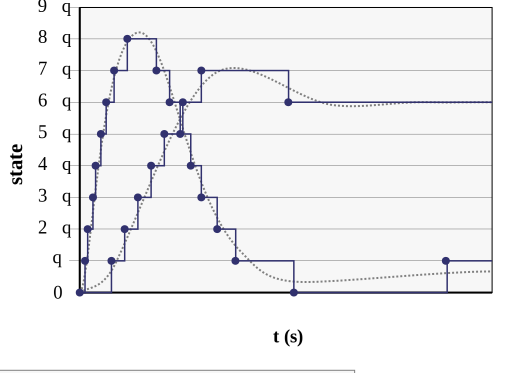
\includegraphics[width=1.0\linewidth]{intro_plots_both.png}
    \caption{Example simulation results for a conceptual $2^{nd}$ order dynamical system, comparing a time-slicing numerical integration method to a quantized state method, where $\Delta t$ is the time step, and $\Delta Q$ is the quantization step size.}
    \label{fig:intro_plots_both}
\end{figure}

In the quantized solution on the right in figure \ref{fig:intro_plots_both}, the quantized state results are not solved synchronously for all system states, and are only defined for each state at multiples of that state's quantization step size ($\Delta Q$). Note that the quantized state solution points are connected with a zero-order hold curve. This is because the results of a $1^{st}$ order quantized state solution are defined as piece-wise constant \cite{kofman2001b} and they are typically rendered accordingly in plots.

\section{Rationale for Applying Quantized State Solutions to Power Systems}

In order to simulate the full range of dynamic behavior in a typical electrical power system with a single dynamical system model, a stiffness ratio ($\lambda_{max} \backslash \lambda_{min}$) of $10^6$ or higher must be supported. Time constants of a power system typically span from the turbo-governor (with time constants on the order of 1 second), to the very fast dynamics of a switching converter (with micro-second time constants). The uniform time-slicing of nodal analysis can potentially simulate such a high-bandwidth system model only by using time steps on the order of micro-seconds. Each of these micro-second time steps requires a full update of the system Jacobian matrix (in the case of non-linear models, which is required for practical, real-world system models). This constant update of the Jacobian matrix forces a constant matrix factorization at each micro-second time step. The computational load (flops per simulation second) for this matrix factorization grows exponentially with increases in system size. For large transmission grids, the electrical node count (and thus the order of the Jacobian matrix) can be as high as hundreds of thousands. Variable time step methods are of little use here, as the simulation of a detailed switching converter requires dense time-slicing between each switch transition, even when the system is in a quasi-steady-state condition.

Quantized state solutions can potentially solve this extreme stiffness problem, and because most of the current literature on quantized state integration revolves around small, linear systems, this is a novel area for research. The simulation of larger, stiffer, and highly non-linear systems is a new area for the application of quantized methods.

\section{Document Outline}

This dissertation will begin in chapter \ref{chap:lim} by describing the Latency Insertion Method, specifically the formulation most relevant to our needs. We cannot apply quantized state solution methods directly to a traditional formulation of a power system. The LIM will allow us to cast the power system model into a form that can be used in a discrete event context by enforcing latency at every system state. The QSS integration concepts are then introduced in chapter \ref{chap:qss}, describing the basic properties of Quantized State Systems. The formal QDEVS specification for a LIM-based system model is then developed in chapter \ref{chap:qdl}, defining the QDEVS functions that operate on a LIM-based system model. The MATLAB and Python implementations of QDL simulations is discussed in chapter \ref{chap:simulator} (with the full source code of these implementations listed in Appendix A).

The next three chapters contain simulations of systems of increasing complexity. Chapter \ref{chap:examples} presents several interesting test cases for the QDL method that demonstrate various properties and advantages of the method. Among these are a 40 state, linear grid of LIM branches and nodes, with an extreme stiffness ratio designed to test the limits of the method. Following those examples, chapters \ref{chap:syncmach} and \ref{chap:powersys} finally apply the QDL method to realistic power system models and systems. Chapter \ref{chap:syncmach} presents a $7^{th}$ order, three-phase synchronous machine attached to an infinite bus. The feasibility of the QDL method for such a model is demonstrated, and the simulation result match the reference simulation very well. The synchronous machine simulation is then used to investigate the relationship between quantization step size and error. Chapter \ref{chap:powersys} applies QDL to a relatively large problem: a multi-machine power system network with 12 device models including cables, buses, a synchronous generator, an induction machine, loads, an (average model) converter, and control devices (an exciter and a governor). This system is complex and realistic enough to test the thesis of this work: to determine if a quantized state method is a feasible and advantageous approach to simulating power system dynamics

Chapter \ref{chap:deltaq} explores the important question of how to select the quantization step size ($\Delta Q$) to optimize simulation performance and control error. A method is proposed to intelligently select $\Delta Q$ based on the propagation of error within the QDL system model. The problems with steady-state behavior of the QDL method is discussed in chapter \ref{chap:steadystate}, along with a proposal for a method of detecting steady-state conditions and mitigating steady-state noise. Finally, chapter \ref{chap:future} describes possible next steps for the research and development of this new method, including further investigation into better methods for selecting $\Delta Q$, a search for better error and noise mitigation, and integrating the most recent, advanced QSS integration methods.



\chapter{Latency Insertion Method}\label{chap:lim}
    
\section{Rationale for using LIM for Quantized State Simulation}

In order to apply Quantized State System (QSS) integration methods, the study system must be described fully by a set of differential equations without any instantaneous coupling between any of the state variables in the system \cite{cellier2008}. To achieve this, we will use a modeling approach called the Latency Insertion Method (LIM). The LIM, described in \cite{schutt2001} exploits existing latency in the network and inserts small, fictitious latency at nodes and branches where no significant physical latency exists. It provides generic node and branch models, that can be combined into arbitrarily complex typologies to model various electrical devices (or any dynamical devices that can be modeled with an equivalent circuit model). The equivalent circuit model representation is powerful because it imposes conservation law inherently, and it is flexible enough to model dynamical subsystems of many engineering disciplines (mechanical, thermal, etc.). 

With latency at every system node and on every system branch, there is no instantaneous coupling between any states. One way to understand this is to imagine a state space system with no off-diagonal components in the state matrix. All of state coupling occurs within a dynamically-updated input vector. And, although there are proposed versions of the LIM for dealing with algebraic sub-networks \cite{sekine2009}, these methods do not create a model that can be QDEVS compliant. We will therefore focus on creating fully latent networks using the original LIM formulation. 

\section{Atomic LIM Components}

The LIM method uses two primary generic components from which the network model can be developed: a LIM \emph{node} and a LIM \emph{branch}. The LIM node defines a KCL-based ODE for the state of a node voltage, and the LIM branch defines a KVL-based ODE for the current flow between two arbitrary nodes. For the QDL method development, we will use the extended LIM node and branch formulations that include dependent sources as described in \cite{goh2011}. This extended formulation provides a straight-forward means of modeling energy-conversion coupling circuits, which are common in power system models.

\begin{figure}[ht]
    \centering
    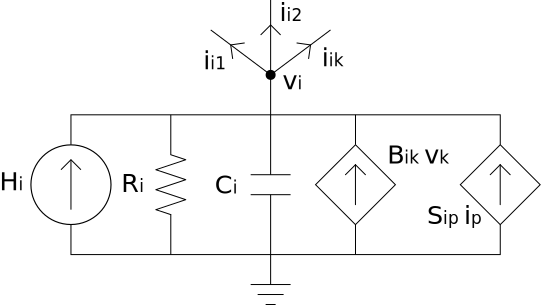
\includegraphics[width=0.7\linewidth]{lim_dependent_node.png}
    \caption{Generic LIM Node with Dependent Sources}
    \label{fig:lim_dependent_node}
\end{figure}

The generic LIM branch model with dependent sources is shown in figure \ref{fig:lim_dependent_node}. The model includes a voltage-controlled current source (VCCS) and a current-controlled current source (CCCS). The KCL equation for the $i^{th}$ node is

\begin{equation} \label{eq:lim_dependent_node}
C_i \frac{d}{dt} v_i(t) + G_i v_i(t) - H_i(t) - B_{ik} v_k(t) - S_{ip} i_p(t) = \sum_{M_i}^{k=1}{i_{ik}(t)}
\end{equation}

Note that these parameters, injections and coefficients can be time-varying and non-linear in general. 

\begin{figure}[ht]
    \label{fig:lim_dependent_branch}
    \centering
    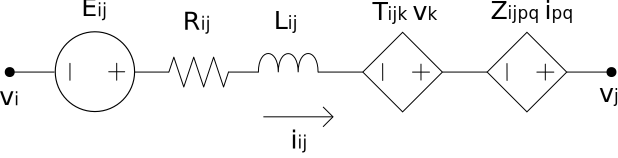
\includegraphics[width=0.8\linewidth]{lim_dependent_branch.png}
    \caption{Generic LIM Branch with Dependent Sources}
\end{figure}

The generic LIM branch model with dependent sources is shown in figure \ref{fig:lim_dependent_branch}. The model includes a voltage-controlled voltage source (VCVS) and a current-controlled voltage source (CCVS). The KVL equation for a branch from $i^{th}$ to the $j^{th}$ node is

\begin{equation} \label{eq:lim_dependent_branch}
v_i(t)-v_j(t) = L_{ij} \frac{d}{dt} i_{ij}(t) + R_{ij} i_{ij}(t) - e_{ij}(t) - T_{ijk}v_k(t) - Z_{ijpq} i_{pq}(t)
\end{equation}

Note that these parameters, injections and coefficients can be time-varying and non-linear in general.  

The LIM formulation also allows for externally-controlled, ideal current source branches and voltage source nodes (see figs. \ref{fig:lim_const_node} and \ref{fig:lim_const_branch}). Although these components are somewhat trivial, they are useful in the derivation of many device models and are worth noting. Because the voltages at the branch ports are effectively dc quantities (as far as the branch model is concerned) during the span of a time step, an ideal source does not require any special consideration by the branch model. Note that ideal voltage nodes may not be added in parallel attached to the same electrical node, and ideal current source branches may not be added in series with other branch models.  

\begin{figure}[ht]
    \label{fig:lim_const_node}
    \centering
    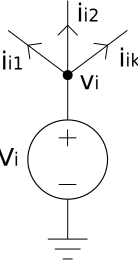
\includegraphics[width=0.18\linewidth]{lim_const_node.png}
    \caption{Ideal Voltage Source Node}
\end{figure}

\begin{figure}[ht]
    \label{fig:lim_const_branch}
    \centering
    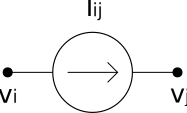
\includegraphics[width=0.24\linewidth]{lim_const_branch.png}
    \caption{Ideal Current Source Branch}
\end{figure}

\section{LIM System Model} 

It is convenient to represent a LIM system model as a state space model, with partitions as shown in (eq. \ref{eq:lim_state_space}). By definition, the LIM state space model does not contain an algebraic output equation but is described fully with the state equation $\dot{\mathbf{x}}(t) = \mathbf{A}\mathbf{x}(t) + \mathbf{B}\mathbf{u}(t)$. The motivation for developing the LIM system state space model is two-fold. We wish to provide a trusted benchmark solution with which to compare QDL simulation accuracy and computational performance, and the state space model is a common format that can be solved with various third-party tools. Also, various components of the LIM state space model will be used directly in the formulation of the QDL atomic model equations described in chapter \ref{chap:qdl}. 

\begin{equation} \label{eq:lim_state_space}
    \frac{d}{dt}
    \begin{bmatrix}
        v \\
        i
    \end{bmatrix}
    = 
    \begin{bmatrix}
        C^{-1}(B-G)   & C^{-1}(S-A) \\
        L^{-1}(T-A^T) & L^{-1}(Z-R)
    \end{bmatrix}
    \begin{bmatrix}
        v \\
        i
    \end{bmatrix}
    +
    \begin{bmatrix}
        C^{-1}  & 0      \\
        0       & L^{-1}
    \end{bmatrix}
    \begin{bmatrix}
        H \\
        E
    \end{bmatrix}
\end{equation}

where: 
\smallskip

$\begin{aligned}
    v & : \text{ the set of node voltages of length } n \\
    i & : \text{ the set of branch currents of length } k \\
    C & : \text{ the set of node shunt capacitance values of length } n \\
    G & : \text{ the set of node shunt conductance values of length } n \\
    H & : \text{ the set of node shunt current injections of length } n \\
    B & : \text{ the set of node VCCS gains of size } (n \times n) \\
    S & : \text{ the set of node CCCS gains of size } (n \times k) \\
    L & : \text{ the set of branch series inductance values of length } k \\
    R & : \text{ the set of branch series resistance values of length } k \\
    E & : \text{ the set of branch series voltage sources of length } k \\
    T & : \text{ the set of branch VCVS gains of size } (k \times n) \\
    Z & : \text{ the set of branch CCVS gains of size } (k \times k) \\
    A & : \text{ the port connection incidence matrix size } (n \times k) \\
\end{aligned}$

\bigskip
and the elements of the incidence matrix $A$ are determined by
\smallskip

\begin{equation} \label{eq:a_matrix}
    A_{i, k} = 
    \begin{cases}
        1,  & \text{if the } i^{th} \text{ node is connected to the } i^{th} \text{ terminal of the } k^{th} \text{ branch }\\ 
        -1, & \text{if the } i^{th} \text{ node is connected to the } j^{th} \text{ terminal of the } k^{th} \text{ branch }\\ 
        0,  & \text{otherwise}
    \end{cases}
\end{equation}

\bigskip

\section{Example LIM System Derivation} 

In order to provide a concrete example of a simple power system formulated using LIM, a dc motor model is presented (fig. \ref{fig:qdl_dc_motor}). This system includes an electro-mechanical energy conversion in the form of back-to-back VCVS and CCCS sources. 

\begin{figure}[ht]
    \label{fig:qdl_dc_motor}
    \centering
    \includegraphics[width=1.0\linewidth]{qdl_dc_motor.png}
    \caption{Example DC Motor System LIM Model with Dependent Sources}
\end{figure}

\bigskip
The LIM system is then defined with the following components:
\bigskip

\begin{equation} \label{eq:lim_sys_1}
v = [v_a \ \ \omega_m \ \ \omega_L]^\intercal,  \ \ \ 
i = [i_a \ \ \tau_s]^\intercal    \\
\end{equation}

\begin{equation} \label{eq:lim_sys_2}
H = [V_g G_g \ \ 0 \ \ T_L]^\intercal,  \ \ \ 
E = [0 \ \ 0]^\intercal    \\
\end{equation}

\begin{multline} \label{eq:lim_sys_3}
R =
\begin{bmatrix}
R_a &  0 \\
0   &  0 \\
\end{bmatrix} ,  \ \ 
L =
\begin{bmatrix}
L_a &  0 \\
0   &  J_p \\
\end{bmatrix} ,  \ \
G =
\begin{bmatrix}
G_g &  0    &  0   \\
0   &  B_m  &  0   \\
0   &  0    &  B_L \\
\end{bmatrix} ,  \ \  \\
C =
\begin{bmatrix}
C_{lim} &  0    &  0   \\
0       &  J_m  &  0   \\
0       &  0    &  J_L \\
\end{bmatrix} ,  \ \
S =
\begin{bmatrix}
0   &  0 \\
K_t &  0 \\
0   &  0 \\
\end{bmatrix} ,  \ \
T =
\begin{bmatrix}
0  &  K_e  &  0  \\
0  &  0    &  0  \\
\end{bmatrix} ,  \ \
A =
\begin{bmatrix}
    1 &  0 \\
    1 &  0 \\
    0 & -1 \\
\end{bmatrix}  
\end{multline}

Note that the armature terminal node does not include any real latency, and so a small, fictitious capacitance of $C_{lim}$ is included in order to ensure that the system has full latency and can be represented by a valid LIM system model. 



\chapter{Quantized State Systems}\label{chap:qss}

The Quantized Discrete Event Specification (QDEVS) \cite{zeigler2018} provides a formal DEVS specification for a discrete event description of quantized systems. The Quantized State System (QSS) methods are a series of integration methods based on the QDEVS specification and described in Zeigler et al. \cite{zeigler2018}. These QSS methods provide a QDEVS-compliant way to simulate continuous systems.

\section{Summary of QSS}

This approach begins with the assumption that a generic continuous state equation system (SES)

\begin{equation} \label{eq:ses}
    \mathbf{\dot x} = f(\mathbf{x}(t), \mathbf{u}(t))
\end{equation}

\noindent can be approximated by a \emph{Quantized} State Systems (QSS) in the form

\begin{equation} \label{eq:qss}
    \mathbf{\dot x} = f(\mathbf{q}(t), \mathbf{u}(t))
\end{equation}

where $\mathbf{q}(t)$ is the quantized state vector that follows a piecewise constant trajectory, and is related to the state vector $\mathbf{x}(t)$ by the quantum size $\Delta Q$. The states are quantized based on their trajectory using various hysteresis quantization functions depending on the specific QSS algorithm used. In \cite{kofman2001} and \cite{cellier1993} the structure and implementation of atomic DEVS models and general-purpose simulators for QSS systems are defined. In the linear case, the QSS approach guarantees a bounded error, \cite{kofman2001b} so analytically stable systems cannot become numerically unstable when being simulated by a fully coupled QSS algorithm. \cite{cellier1993} Several variations of QSS offer different features. The simplest formulation, QSS1, developed in Zeigler et al. \cite{zeigler2018}, and Kofman and Junco \cite{kofman2001b}, relies on explicit integration and uses first-order estimates of state derivatives to predict the time at which the continuous state $x_i(t)$ will increase or decrease by amount $\Delta Q$ (quantization step size) from the current quantized value $q_i(t)$ to the next higher or lower quantized value.

\section{QSS Method Selection for QDL}

Although QSS1 has some advantages, such as being easy to implement, its disadvantage is that it uses a first-order approximation of the state trajectory to calculate the time to the next event. To get accurate results, $\Delta Q$ has to be quite small, which produces a large number of steps. The QSS2 \cite{kofman2002} and QSS3 \cite{kofman2006} methods use more accurate second- and third-order approximations, respectively, for the state trajectory, however, the computational cost grows with the square root and cubic root of the desired accuracy. Because we are interested in simulating realistic, stiff power systems that include both fast electrical dynamics and slow mechanical dynamics, we require a QSS method that can handle stiff systems. This requirement eliminates QSS1, QSS2, and QSS3 because these methods create fictitious high-frequency oscillations for stiff systems which in turn generate large numbers of steps. These steps are costly in computational cost and memory size, even when a system is nominally in steady state. To address this, a Linear-Implicit QSS (LIQSS1) algorithm is used as proposed in \cite{migoni2009}. The LIQSS1 method uses a semi-implicit solution in the quantization function to force steady-state derivatives to zero and prevent troublesome oscillations for stiff systems. We will use the LIQSS1 algorithm for the development of the QDL method in the following chapter.



\chapter{The Quantized DEVS-LIM (QDL) Method}\label{chap:qdl}

The formal QDEVS function definitions for the proposed QDL method are presented in this chapter.

\section{QDL QDEVS Specification}

The original DEVS specification is outlined in \cite{zeigler2002}, and further developed for quantized systems (QDEVS) in \cite{zeigler1999}. The specification consists of several functions that need to be defined for a specific QDEVS model. These are

\begin{align*}
    f            & \text{:   Derivative Update function} \\
    \delta_{int} & \text{:   Internal State Transition Function} \\
    \delta_{ext} & \text{:   External State Transition Function} \\
    ta           & \text{:   Time Advance Function, and} \\
    Q            & \text{:   Quantization Function.}  \\
\end{align*}

These are defined below for the LIM atomic models presented in chapter \ref{chap:lim}, and for the LIQSS1 integration method in \cite{migoni2013}.

\subsection{QDL Derivative Update Function}

The derivative estimate is then determined from the LIM model for the nodes with

\begin{equation}\label{eq:d_func_node}
    d_i = \frac{H_{ii}}{C_{ii}} - \frac{G_{ii}}{C_{ii}} \cdot q_i + \frac{1}{C_{ii}} B_i \cdot q^{node} + \frac{1}{C_{ii}} \left(S_i - A_i\right) \cdot q^{branch},
\end{equation}

\noindent and for the branches with

\begin{equation}\label{eq:d_func_branch}
    d_k = \frac{E_{kk}}{L_{kk}} - \frac{R_{kk}}{L_{kk}} \cdot q_k + \frac{1}{L_{kk}} Z_k \cdot q^{node} + \frac{1}{L_{kk}} \left(T_k - A_k^T\right) \cdot q^{branch}, 
\end{equation}

\noindent where $C_{ii}$, $G_{ii}$, $H_{ii}$, $R_{kk}$, $L_{kk}$, and $E_{kk}$, are quantities from the LIM model at node $i$ and branch $k$. $B_i$, $S_i$, and $B_i$ are quantities from the LIM model at row $i$. $Z_k$, $T_k$, and $Z_k$ quantities from the LIM model at row $k$. $q_i$ is the quantized state at node $i$, $q_k$ is the quantized state at branch $k$, $q^{node}$ is the vector of node quantized states, and $q^{branch}$ is the vector of branch quantized states.

\subsection{QDL Internal State Transition Function} 

The internal state for each QDL atom is calculated by the internal transition function $\delta_{int}$. An internal transition occurs when the simulation time has advanced to the atom's $t^{next}$ value determined by its time advance function $ta$.

\noindent In this function, the node voltage states are updated as

\begin{equation}\label{eq:delta_int_node}
    v_i = v_i^{last} + d_i^{last} \cdot \left(t - t_i^{last}\right),
\end{equation}

\noindent and the branch currents are updated as

\begin{equation}\label{eq:delta_int_branch}
    i_k = i_k^{last} + d_k^{last} \cdot \left(t - t_k^{last}\right),
\end{equation}

\noindent where $v_i$ and $i_k$ are the voltage at node $i$ and the current at branch $k$ respectively.

\noindent After the states are updated, the $t^{last}$ values are saved:

\begin{equation} \label{eq:delta_int_save}
    t_i^{last} = t, \ \ t_k^{last} = t.
\end{equation}

\subsection{QDL External State Transition Function} 

In the case of QDL, the \emph{behavior} of the internal $\delta_{int}$ and the external $\delta_{ext}$ transition functions are identical. The difference is in how each is invoked. The internal transition is triggered when the simulation time $t$ has advanced to the atom's $t^{next}$ value determined in the $ta$ function, and the external transition is triggered when one or more connected atoms' quantized states change. Because the behavior of the internal and external transition functions is identical, the confluent transition function $\delta_{con}$ is not required.

\subsection{QDL Time Advance Function} 

The time until the next internal transition is determined from the time advance function $ta$. 

\noindent The time advance calculation for node $i$ is

\begin{equation} \label{eq:ta_node}
    t_i^{next} = 
    \begin{cases}
        t_i + ( \bar{q}_i - v_i ) \slash {d_i}, & \text{ if } d_i^{last} > 0 \\
        t_i + ( \underline{q}_i - v_i ) \slash {d_i}, & \text{ if } d_i^{last} < 0 \\
        \infty, &\text{ otherwise}
    \end{cases},
\end{equation}

\noindent and for branch $k$ is

\begin{equation} \label{eq:ta_branch}
    t_k^{next} = 
    \begin{cases}
        t_k + ( \bar{q}_k - i_k ) \slash {d_k}, & \text{ if } d_k(t_k^{last}) > 0 \\
        t_k + ( \underline{q}_k - i_k ) \slash {d_k}, & \text{ if } d_k(t_k^{last}) < 0 \\
        \infty, &\text{ otherwise}
    \end{cases},
\end{equation}

\noindent where $\bar{q}$ and $\underline{q}$ are the upper and lower quantization limits respectively, and are dynamically updated by the quantization function described in the following section. 

\subsection{QDL Quantization Function} 

The quantization function quantizes the internal state after a transition has occurred. The LIQSS1 method uses an advanced hysteresis function that tracks the sign of the derivative, determines when the state is oscillating between two quantized levels ($\pm \Delta Q$), and sets the quantized value such that the derivative is zero, using an approximation of the Jacobian diagonal. Below is the description of the LIQSS1 atomic DEVS model quantization method which is described in \cite{migoni2009}.

Note that the quantization function is the same for node voltages and branch currents, but only the equations for $\mathbf{v}$ and $v_i$ are included below for brevity. The same equations apply to the branch currents by substituting $\mathbf{i}$ and $i_k$ in place of $\mathbf{v}$ and $v_i$.

The following definitions will be used in the description of the quantization function:

\begin{align*}
    \mathbf{v}      & \text{ is the set of node voltages}, \\
    \mathbf{u}      & \text{ is the set of external inputs}, \\
    \mathbf{q}      & \text{ is the set of quantized states of all nodes and branches}, \\
    \mathbf{J}      & \text{ is the Jacobian matrix}, \\
    v_i             & \text{ is the value for the } i^{th} \text{ voltage at time } t, \\
    \dot{v}_i       & \text{ is the time derivative of } v_i, \\
    f_i             & \text{ is the time derivative function of } v_i,
\end{align*}

\begin{align*}
    \Delta Q_i      & \text{ is the quantization step size for the } i^{th} \text{ node}, \\
    q_i             & \text{ is the quantized value of } v_i, \\
    \underline{q}_i & \text{ is the lower quantum limit of } v_i, \\
    \bar{q}_i       & \text{ is the upper quantum limit of } v_i, \\
    \hat{q}_i       & \text{ is the quantized value for which } \dot{v}_i=0, \text{ and} \\
    \tilde{q}_i     & \text{ is the approximate quantized value for which } \dot{v}_i=0.
\end{align*}

Note that the dependence of $v$, $u$, and $q$ on the current simulation time $t$ is implicit, except where the superscript $last$ is used to denote quantities at the simulation time $t^-$, or the time of the previous quantization update.

\begin{equation}
    \label{eq:liqss_qfunc}
    q_i = 
    \begin{cases}
        
        \underline{q}_i, & \text{if } f_i \left( \mathbf{q}, \mathbf{u} \right) \left( \underline{q}_i - v_i \right) \geq 0 \\
        
        \bar{q}_i, & \text{if } f_i \left( \mathbf{q}, \mathbf{u} \right) \left( \bar{q}_i - v_i \right) \geq 0 \wedge f_i \left( \mathbf{q}, \mathbf{u} \right) \left( \underline{q}_i - v_i \right) < 0\\
        
        \tilde{q}_i, & \text{otherwise}
        
    \end{cases} \text{   ,} 
\end{equation}

\noindent with the upper and lower quantized limits defined as

\begin{equation}
    \label{eq:liqss_qlow}
    \underline{q}_i = 
    \begin{cases}
        
        \underline{q}_i^{last}-\Delta Q_i, & \text{if } v_i-\underline{q}_i^{last} \leq 0 \\
        
        \underline{q}_i^{last}+\Delta Q_i, & \text{if } v_i-\underline{q}_i^{last} \geq 2 \Delta Q_i \\
        
        \underline{q}_i^{last}, & \text{otherwise}
        
    \end{cases} \text{   ,} 
\end{equation}

\begin{equation}
    \label{eq:liqss_qhigh}  
    \bar{q}_i = \underline{q}_i^{last} + 2 \Delta Q_i, \text{ and}
\end{equation}

\begin{equation} \label{eq:liqss_qtilde}  
    \tilde{q}_i = 
    \begin{cases}
        
        \bar{q}_i - (1/A_{ii}) \cdot f_i \left( \bar{\mathbf{q}}^i \right), & \text{if } J_{ii} \ne 0 \\
        
        q_i^{last}, & \text{otherwise}
        
    \end{cases}  \text{   ,} 
\end{equation}

\noindent where $\bar{\mathbf{q}}^i$ is equal to $\mathbf{q}^{last}$ except for the $i^{th}$ component, where it is equal to $\bar{q}_i$ and $J_{ii}$ is the $ii^{th}$ component of the Jacobian matrix evaluated at $\bar{\mathbf{q}}^i$, .i.e.,

\begin{equation}
    \label{eq:liqss_qtilde2}  
    J_{ii} = \left. \frac{\partial f_i}{\partial v_i} \right|_{\bar{\mathbf{q}}^i, u^{last}},
\end{equation}

\noindent and therefore, when $J_{ii} \ne 0$, setting $q_i = \tilde{q}_i$ will force $\dot{v}_i=0$ in the linear case. The calculation of $\tilde{q}_i$ is achieved by taking $\hat{\mathbf{q}}^i$ equal to $\bar{\mathbf{q}}^i$ except for the $i^{th}$ component is $\hat{q}_i$.

We solve for $\hat{q}$ (the point where $f_i=0$) as 

\begin{equation}
    \label{eq:liqss_qhat3}  
    \hat{q}_i = \bar{q}_i - \frac{f_i \left( \bar{\mathbf{q}}^i, \mathbf{u} \right) }{J_{ii}} + \frac{g \left( \bar{\mathbf{q}}^i, \mathbf{u} \right) - q \left( \hat{\mathbf{q}}^i, \mathbf{u} \right) }{J_{ii}},
\end{equation}

where $g(\mathbf{x}, \mathbf{u}) = f(\mathbf{x}, \mathbf{u}) - J_i \cdot \mathbf{x}$, $J_{ii}$ is approximated by

\begin{equation}
    \label{eq:liqss_Jii}
    J_{ii} \approx \frac{f_i \left( \bar{\mathbf{q}}^i, \mathbf{u} \right) - f_i \left( \underline{\mathbf{q}}^i, \mathbf{u} \right) }{\bar{q}_i - \underline{q}_i}.
\end{equation}

\subsection{Simulation Procedure} 

The atomic models are coupled via the topological connections as encoded in the LIM system port connection incidence matrix $A$, as well as the controlled source matrices $B$, $S$, $T$ and $Z$ (see eq. \ref{eq:lim_state_space}). These coupled models become the Coupled DEVS System as described in \cite{zeigler1999} and \cite{kofman2004}. For the simple but illustrative case of two coupled LIM atoms, a node and a branch, the data flow can be visualized as in figure \ref{fig:lim_sys1_qdevs}. Each atom maintains its internal state, and broadcasts changes in its external quantized state to the other atom via an event queue that manages the internal and external events of both atoms.

\begin{figure}[htb]
    \centering
    \includegraphics[width=0.75\textwidth]{lim_sys1_qdevs_ver2.png}
    \caption{$2^{nd}$ order QDL system data flow.}
    \label{fig:lim_sys1_qdevs}
\end{figure}

The full DEVS simulation procedure that implements the Coupled DEVS simulation is described in the flow chart in \ref{fig:qdl_flowchart}.

\begin{figure}[htb]
    \centering
    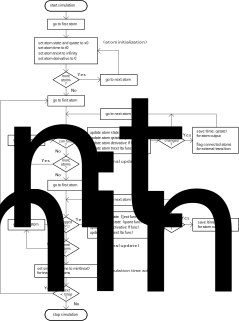
\includegraphics[width=1.0\textwidth]{qdl_flowchart.pdf}
    \caption{Simplified QDL simulation procedure flowchart.}
    \label{fig:qdl_flowchart}
\end{figure}



\chapter{QDL Simulator Implementations}\label{chap:simulator}

Two implementations have been developed for simulating systems with the QDL method; a MATLAB implementation for efficient simulation of linear systems, and a Python implementation for fast prototyping of a QDL simulator that can support non-linear models and advanced QSS integration methods. 

\section{MATLAB QDL Implementation} 

An object-oriented implementation of a QDL simulator was implemented in MATLAB script that is suitable for linear QDL system models. The full source code of this implementation is included in Appendix \ref{chap:matlab_source}. 

The key objects of the MATLAB script QDL implementation are

\begin{itemize}
    \item{\textbf{QdlSystem}: Contains the collection of QDL atom objects, the system matrices, the main simulator algorithm, stimulus implementations and plotting utilities.}
    \item{\textbf{QdlNode}: The generic QDL node atom model}
    \item{\textbf{QdlBranch}: The generic QDL branch atom model}
    \item{\textbf{QdlSimulum}: The generic QDL stimulus interface.}
\end{itemize}

Example source code for a QDL simulation system definition is listed below for a 30 second simulation of a dc motor. The motor is excited by a PWM voltage source and loaded with a  torque load that steps from $0$ to $0.5 Nm$ at $10$ seconds. 

\bigskip

\begin{lstlisting}
dQ = 0.1

Va = 10;
Ra = 0.1;
La = 0.01;
Ke = 0.1;
Kt = 0.1;
Jm = 0.1;
Bm = 0.001;
Tm = 0.0;

sys = QdlSystem(dQ);

va = QdlNode('va (V) (100Hz d=0.5)', 0, 0, 0);
va.stim_type = QdlSystem.StimSource;
va.source_type = QdlSystem.SourcePWM;
va.freq = 100; 
va.duty = 0.5; 
va.v1 = Va; 
va.v2 = 0; 

gnd = QdlNode('ground', 0, 0, 0);
gnd.stim_type = QdlSystem.StimSource;
gnd.source_type = QdlSystem.SourceDC;
gnd.vdc = 0.0; 

nmech = QdlNode('shaft speed (rad/s)', Jm, Bm, Tm);

barm = QdlBranch('armature current (A)', La, Ra, 0);
barm.connect(va, gnd);

barm.add_tnode(nmech, -Ke);
nmech.add_sbranch(barm, Kt);

sys.add_node(va);
sys.add_node(gnd);
sys.add_node(nmech);
sys.add_branch(barm);

sys.init();
sys.runto(10);
sys.H(3) = -0.5;  % step load torque
sys.runto(20);
    
\end{lstlisting}

The node and branch device constructors have arguments for the primary component coefficients (namely $L$, $R$, $E$, $C$, $B$, and $H$), and the controlled source connections are realized via add\_tnode(), add\_zbranch(), add\_sbranch() and add\_bnode() functions for the branch and node atoms. This allows an arbitrary number of controlled sources to be added to the node and branch atoms. The simulator is run via the runto() function, that can be called multiple times sequentially, allowing discrete event changes to be introduced to any system variable during the simulation. Various quantized source types are available. Used here is a PWM source. These sources create discrete events that are pushed into the event queue along with the QSS integrator scheduled events.

\section{Python QDL Implementation} 

For the fast prototyping of more advanced integrators, quantizers, sources, devices and system models, Python was chosen as the language of choice. The full source code of this implementation is included in Appendix \ref{chap:python_source}. 

The key objects of the Python QDL framework are

\begin{itemize}
    \item{\textbf{qdl.System}: Contains the collection of QDL device objects, the main simulator algorithms, reference ODE solutions, stimulus implementations and plotting utilities.}
    \item{\textbf{qdl.Atom}: A generic QDL atom model}
    \item{\textbf{qdl.StateAtom}: A QDL state atom model where the QDEVS functions are implemented.}
    \item{\textbf{qdl.SourceAtom}: A source atom model for quantized input signal components, and}
    \item{\textbf{qdl.Device}: The generic QDL device interface, a collection of QDL atoms, connection ports, time derivative and Jacobian cell functions.}
\end{itemize}

In addition to the framework objects, the Python QDL implementation also has an extensive hierarchical device library, including complex devices such as the three-phase electric machines used in chapters \ref{chap:syncmach} and \ref{chap:powersys}.

As a first example of QDL Python model definitions, the LIM Branch and Node components are listed below. The LIM atom coefficients and Jacobian matrix components are determined at run time using delegate functions (such as $a_{ii}$, and $b_{ij}$, etc.), allowing non-linear and time-varying behavior to be modeled.

\bigskip 

\begin{lstlisting}
class LimNode(Device):

    def __init__(self, name, c, g=0.0, h0=0.0, v0=0.0,
                 source_type=SourceType.CONSTANT, h1=0.0,
                 h2=0.0, ha=0.0, freq=0.0, phi=0.0, duty=0.0,
                 t1=0.0, t2=0.0, dq=None):

        Device.__init__(self, name)

        self.c = c
        self.g = g

        self.h = SourceAtom("h", source_type=source_type,
                            x0=h0, x1=h1, x2=h2, xa=ha,
                            freq=freq, phi=phi, duty=duty,
                            t1=t1, t2=t2, dq=dq, units="A")

        self.voltage = StateAtom("voltage", x0=0.0,
                                 coeffunc=self.aii,
                                 dq=dq, units="V")

        self.add_atoms(self.h, self.voltage)
        
        self.voltage.add_connection(self.h, coeffunc=self.bii)
        
        self.voltage.add_jacfunc(self.voltage, self.aii)

    def connect(self, branch, terminal="i"):

        if terminal == "i":
            self.voltage.add_connection(branch.current, 
                                        coeffunc=self.aij)
                                        
            self.voltage.add_jacfunc(branch.current, self.aij)

        elif terminal == "j":
            self.voltage.add_connection(branch.current,  
                                        coeffunc=self.aji)
                                        
            self.voltage.add_jacfunc(branch.current, self.aji)

    def aii(self, v):
        return -self.g / self.c

    def bii(self):
        return 1.0 / self.c

    def aij(self, v, i):
        return -1.0 / self.c

    def aji(self, i, v):
        return 1.0 / self.c


class LimBranch(Device):

    def __init__(self, name, l, r=0.0, e0=0.0, i0=0.0,
                 source_type=SourceType.CONSTANT, e1=0.0,
                 e2=0.0, ea=0.0, freq=0.0, phi=0.0,
                 duty=0.0, t1=0.0, t2=0.0, dq=None):

        Device.__init__(self, name)

        self.l = l
        self.r = r

        self.e = SourceAtom("e", source_type=source_type,
                            x0=e0, x1=e1, x2=e2, xa=ea,
                            freq=freq, phi=phi, duty=duty,
                            t1=t1, t2=t2, dq=dq, units="V")

        self.current = StateAtom("current", x0=0.0,
                                 coeffunc=self.aii,
                                 dq=dq, units="A")

        self.add_atoms(self.e, self.current)
        
        self.current.add_connection(self.e,
                                    coeffunc=self.bii)
        
        self.current.add_jacfunc(self.current, self.aii)

    def connect(self, inode, jnode):

        self.current.add_connection(inode.voltage,
                                    coeffunc=self.aij)
        
        self.current.add_connection(jnode.voltage,
                                    coeffunc=self.aji)
        
        self.current.add_jacfunc(inode.voltage, self.aij)
        self.current.add_jacfunc(jnode.voltage, self.aji)

    def aii(self, i):
        return -self.r / self.l

    def bii(self):
        return 1.0 / self.l

    def aij(self, i, v):
        return 1.0 / self.l

    def aji(self, v, i):
        return -1.0 / self.l
\end{lstlisting}

As an example of a more complex device, the source for the Synchronous Machine in the DQ frame is listed below. This example contains many complex derivatives and Jacobian matrix components encoded in delegate functions in the Python class definition.

\bigskip

\begin{lstlisting}
class SyncMachineDQ(Device):

    def __init__(self, name, Psm=25.0e6, VLL=4160.0, ws=60.0*PI,
        P=4, pf=0.80, rs=3.00e-3, Lls=0.20e-3, Lmq=2.00e-3,
        Lmd=2.00e-3, rkq=5.00e-3, Llkq=0.04e-3, rkd=5.00e-3,
        Llkd=0.04e-3, rfd=20.0e-3, Llfd=0.15e-3, vfdb=90.1,
        Kp=10.0e4, Ki=10.0e4, J=4221.7, fkq0=0.0, fkd0=0.0,
        ffd0=0.0, wr0=60.0*PI, th0=0.0, iqs0=0.0, ids0=0.0,
        dq_i=1e-2, dq_f=1e-2, dq_wr=1e-1, dq_th=1e-3, dq_v=1e0):
        
        self.name = name  
        Device.__init__(self, name)
        
        self.Psm  = Psm
        self.VLL  = VLL
        self.ws   = ws
        self.P    = P
        self.pf   = pf
        self.rs   = rs
        self.Lls  = Lls
        self.Lmq  = Lmq
        self.Lmd  = Lmd
        self.rkq  = rkq
        self.Llkq = Llkq
        self.rkd  = rkd
        self.Llkd = Llkd
        self.rfd  = rfd
        self.Llfd = Llfd
        self.vfdb = vfdb
        self.Kp   = Kp
        self.Ki   = Ki
        self.J    = J
        
        # set intial conditions:
        
        self.iqs0 = iqs0
        self.ids0 = ids0
        self.fkq0 = fkq0
        self.fkd0 = fkd0
        self.ffd0 = ffd0
        self.wr0  = wr0
        self.th0  = th0 
        
        # cached derived impedances:
        
        self.Lq = Lls + (Lmq * Llkq) / (Llkq + Lmq)
        self.Ld = (Lls + (Lmd * Llfd * Llkd) 
                  / (Lmd * Llfd + Lmd * Llkd + Llfd * Llkd))
        
        # atoms:
        
        self.ids = StateAtom("ids", x0=ids0, derfunc=self.dids,
                             units="A",     dq=dq_i)
                             
        self.iqs = StateAtom("iqs", x0=iqs0, derfunc=self.diqs, 
                             units="A",     dq=dq_i)
                             
        self.fkq = StateAtom("fkq", x0=fkq0, derfunc=self.dfkq, 
                             units="Wb",    dq=dq_f)
                             
        self.fkd = StateAtom("fkd", x0=fkd0, derfunc=self.dfkd, 
                             units="Wb",    dq=dq_f)
                             
        self.ffd = StateAtom("ffd", x0=ffd0, derfunc=self.dffd,
                             units="Wb",    dq=dq_f)
                             
        self.wr  = StateAtom("wr",  x0=wr0,  derfunc=self.dwr,
                             units="rad/s", dq=dq_wr)
                             
        self.th  = StateAtom("th",  x0=th0,  derfunc=self.dth, 
                             units="rad",   dq=dq_th)
        
        self.add_atoms(self.ids, self.iqs, self.fkq, self.fkd,
                       self.ffd, self.wr,  self.th)
        
        # internal connections:
        
        self.ids.add_connection(self.iqs)
        self.ids.add_connection(self.wr )
        self.ids.add_connection(self.fkq)   
        self.iqs.add_connection(self.ids)
        self.iqs.add_connection(self.wr )
        self.iqs.add_connection(self.fkd)
        self.iqs.add_connection(self.ffd)      
        self.fkd.add_connection(self.ffd)
        self.fkd.add_connection(self.ids)
        self.fkq.add_connection(self.iqs)       
        self.ffd.add_connection(self.ids)
        self.ffd.add_connection(self.fkd)      
        self.wr.add_connection( self.ids)
        self.wr.add_connection( self.iqs)
        self.wr.add_connection( self.fkq)
        self.wr.add_connection( self.fkd)
        self.wr.add_connection( self.ffd)
        self.wr.add_connection( self.th )
        self.th.add_connection( self.wr )
        
        # jacobian:
        
        self.ids.add_jacfunc(self.ids, self.jids_ids)
        self.ids.add_jacfunc(self.iqs, self.jids_iqs)
        self.ids.add_jacfunc(self.fkq, self.jids_fkq)
        self.ids.add_jacfunc(self.wr , self.jids_wr )    
        self.iqs.add_jacfunc(self.ids, self.jiqs_ids)
        self.iqs.add_jacfunc(self.iqs, self.jiqs_iqs)
        self.iqs.add_jacfunc(self.fkd, self.jiqs_fkd)
        self.iqs.add_jacfunc(self.ffd, self.jiqs_ffd)
        self.iqs.add_jacfunc(self.wr , self.jiqs_wr )       
        self.fkq.add_jacfunc(self.iqs, self.jfkq_iqs)
        self.fkq.add_jacfunc(self.fkq, self.jfkq_fkq)     
        self.fkd.add_jacfunc(self.ids, self.jfkd_ids)
        self.fkd.add_jacfunc(self.fkd, self.jfkd_fkd)
        self.fkd.add_jacfunc(self.ffd, self.jfkd_ffd)    
        self.ffd.add_jacfunc(self.ids, self.jffd_ids)
        self.ffd.add_jacfunc(self.fkd, self.jffd_fkd)
        self.ffd.add_jacfunc(self.ffd, self.jffd_ffd)        
        self.wr.add_jacfunc( self.wr , self.jwr_wr  )
        self.wr.add_jacfunc( self.ids, self.jwr_ids )
        self.wr.add_jacfunc( self.iqs, self.jwr_iqs )
        self.wr.add_jacfunc( self.fkq, self.jwr_fkq )
        self.wr.add_jacfunc( self.fkd, self.jwr_fkd )
        self.wr.add_jacfunc( self.ffd, self.jwr_ffd )
        self.wr.add_jacfunc( self.th , self.jwr_th  )       
        self.th.add_jacfunc( self.wr , self.jth_wr  )
        
        # DQ ports:
        
        self.id = self.iqs
        self.iq = self.ids
        self.vd = None
        self.vq = None
        
        # input port:
        
        self.input = None  # avr output vref connection 
    
    def connect(self, bus, avr):
    
        self.vd = self.iqs.add_connection(bus.vq)
        self.vq = self.ids.add_connection(bus.vd)
        self.input = self.ffd.add_connection(avr.vfd, self.vfdb)
        
        self.iqs.add_jacfunc(bus.vq, self.jiqs_vq)
        self.ids.add_jacfunc(bus.vd, self.jids_vd)
        self.ffd.add_jacfunc(avr.vfd, self.jffd_vfd)
    
    def vtermd(self):
        return self.vd.value()
    
    def vtermq(self):
        return self.vq.value()
    
    def vfd(self):
        return self.input.value()
    
    # Jacobian functions:
    
    def jffd_vfd(self, ffd, vfd):
        return self.vfdb
        
    def jids_vd(self, ids, vd):
        return -1 / self.Lls
        
    def jiqs_vq(self, iqs, vq):
        return -1 / self.Lls
        
    def jids_ids(self, ids):
        return -self.rs/self.Lls
        
    def jids_iqs(self, ids, iqs):
        return -(self.Lq * self.wr.q) / self.Lls
        
    def jids_fkq(self, ids, fkq):
        return (self.Lmq * self.wr.q) / (self.Lls
        * (self.Lmq + self.Llkq))
        
    def jids_wr(self, ids, wr):
        return (((self.Lmq * self.fkq.q)
        / (self.Lmq + self.Llkq)
        - self.Lq * self.iqs.q) / self.Lls)
        
    def jiqs_ids(self, iqs, ids):
        return (self.Ld * self.wr.q) / self.Lls
        
    def jiqs_iqs(self, iqs):
        return -self.rs / self.Lls
        
    def jiqs_fkd(self, iqs, fkd):
        return ((self.Lmd * self.wr.q) / (self.Llkd 
        * self.Lls * (self.Lmd / self.Llkd + self.Lmd
        / self.Llfd + 1)))
        
    def jiqs_ffd(self, iqs, ffd):
        return ((self.Lmd * self.wr.q) / (self.Llfd
        * self.Lls * (self.Lmd / self.Llkd + self.Lmd
        / self.Llfd + 1)))
        
    def jiqs_wr(self, iqs, wr):
        return ((self.Ld * self.ids.q + (self.Lmd
        * (self.fkd.q / self.Llkd + self.ffd.q
        / self.Llfd)) / (self.Lmd / self.Llkd
        + self.Lmd / self.Llfd + 1)) / self.Lls)
        
    def jfkq_iqs(self, fkq, iqs):
        return -((self.Lls - self.Lq) * self.rkq)
        / self.Llkq
        
    def jfkq_fkq(self, fkq):
        return -((1 - self.Lmq / (self.Lmq
        + self.Llkq)) * self.rkq) / self.Llkq
        
    def jfkd_ids(self, fkd, ids):
        return -((-self.Lls - self.Ld)
        * self.rkd) / self.Llkd
        
    def jfkd_fkd(self, fkd):
        return (-((self.Lmd / (self.Llkd * (self.Lmd
        / self.Llkd + self.Lmd / self.Llfd + 1)) + 1)
        * self.rkd) / self.Llkd)
        
    def jfkd_ffd(self, fkd, ffd):
        return -(self.Lmd * self.rkd) / (self.Llfd
        * self.Llkd * (self.Lmd / self.Llkd
        + self.Lmd / self.Llfd + 1))
        
    def jffd_ids(self, ffd, ids):
        return -((-self.Lls - self.Ld) * self.rfd)
        / self.Llfd
        
    def jffd_fkd(self, ffd, fkd):
        return (-(self.Lmd * self.rfd) / (self.Llfd
        * self.Llkd * (self.Lmd / self.Llkd + self.Lmd
        / self.Llfd + 1)))
        
    def jffd_ffd(self, ffd):
        return (-((self.Lmd / (self.Llfd * (self.Lmd 
        / self.Llkd + self.Lmd / self.Llfd + 1)) + 1)
        * self.rfd) / self.Llfd)
        
    def jwr_ids(self, wr, ids):
        return ((0.75*self.P*(-self.Lq*self.iqs.q+self.Ld
        * self.iqs.q-(self.Lmq*self.fkq.q)/(self.Lmq
        + self.Llkq)))/self.J)
        
    def jwr_iqs(self, wr, iqs):
        return ((0.75*self.P*(-self.Lq*self.ids.q+self.Ld
        * self.ids.q+(self.Lmd*(self.fkd.q/self.Llkd
        + self.ffd.q/self.Llfd))/(self.Lmd/self.Llkd
        + self.Lmd/self.Llfd+1.0)))/self.J)
        
    def jwr_fkq(self, wr, fkq):
        return (-(0.75 * self.Lmq * self.P * self.ids.q)
        / (self.J * (self.Lmq + self.Llkq)))
        
    def jwr_fkd(self, wr, fkd):
        return ((0.75 * self.Lmd * self.P * self.iqs.q)
        / (self.J * self.Llkd * (self.Lmd / self.Llkd
        + self.Lmd / self.Llfd + 1)))
        
    def jwr_ffd(self, wr, ffd):
        return ((0.75 * self.Lmd * self.P * self.iqs.q)
        / (self.J * self.Llfd * (self.Lmd / self.Llkd
        + self.Lmd / self.Llfd + 1)))
        
    def jwr_wr(self, wr):
        return -self.Kp / self.J
        
    def jwr_th(self, wr, fthkq):
        return self.Ki / self.J
        
    def jth_wr(self, th, wr):
        return -1.0
        
    # derivative functions:
        
    def dids(self, ids):
        return ((-self.wr.q * self.Lq * self.iqs.q + self.wr.q
        * (self.Lmq / (self.Lmq + self.Llkq) * self.fkq.q)
        - self.vtermd() - self.rs * ids) / self.Lls)
        
    def diqs(self, iqs):
        return ((self.wr.q * self.Ld * self.ids.q + self.wr.q
        * (self.Lmd * (self.fkd.q / self.Llkd + self.ffd.q
        / self.Llfd) / (1.0 + self.Lmd / self.Llfd + self.Lmd
        / self.Llkd))
        - self.vtermq() - self.rs * iqs) / self.Lls)
        
    def dfkq(self, fkq):
        return (-self.rkq / self.Llkq * (fkq - self.Lq
        * self.iqs.q - (self.Lmq / (self.Lmq + self.Llkq)
        * fkq) + self.Lls * self.iqs.q))
        
    def dfkd(self, fkd):
        return (-self.rkd / self.Llkd * (fkd - self.Ld
        * self.ids.q + (self.Lmd * (fkd / self.Llkd
        + self.ffd.q / self.Llfd) / (1.0 + self.Lmd
        / self.Llfd + self.Lmd / self.Llkd)) - self.Lls
        * self.ids.q))
        
    def dffd(self, ffd):
        return (self.vfd() - self.rfd / self.Llfd
        * (ffd - self.Ld * self.ids.q + (self.Lmd
        * (self.fkd.q / self.Llkd + ffd / self.Llfd)
        / (1.0 + self.Lmd / self.Llfd + self.Lmd
        / self.Llkd)) - self.Lls * self.ids.q))
        
    def dwr(self, wr):
        return ((3.0 * self.P / 4.0 * ((self.Ld
        * self.ids.q + ((self.Lmd * (self.fkd.q
        / self.Llkd + self.ffd.q / self.Llfd)
        / (1.0 + self.Lmd / self.Llfd + self.Lmd
        / self.Llkd)))) * self.iqs.q - (self.Lq
        * self.iqs.q + (self.Lmq / (self.Lmq
        + self.Llkq) * self.fkq.q)) * self.ids.q))
        + (self.Kp * (self.ws - wr) + self.Ki
        * self.th.q)) / self.J
        
    def dth(self, th):
        return (self.ws - self.wr.q)
\end{lstlisting}

A system simulation is defined in a Python script. An example simulation script is listed below for a similar dc motor system as the previous MATLAB example.

\bigskip

\begin{lstlisting}
dq = 1e-2
f = 100.0
d = 0.5

sys = System()

ground = GroundNode("ground")
source = PwmSourceNode("source", vlo=0.0, vhi=1.0, freq=f, duty=d)
                        
motor = DCMotor("motor", ra=0.1, La=0.01, Jm=0.1, Bm=0.001, Kt=0.1,
                 Ke=0.1, ia0=0.0, wr0=0.0, dq_ia=dq, dq_wr=dq)

motor.connect(source, ground)

sys.add_devices(ground, source, motor)

tstop = 10.0
dt = 1e-4
dc = True
optimize_dq = 0
ode = True
qss = True

chk_ss_delay = 2.0

def event(sys):
    source.voltage.duty = 0.8

sys.schedule(event, tstop*0.5)

sys.initialize(dt=dt, dc=dc)

sys.run(tstop, ode=ode, qss=qss, verbose=True, ode_method="LSODA",
        optimize_dq=optimize_dq, chk_ss_delay=chk_ss_delay)

\end{lstlisting}

To define a system in the Python implementation, the device models are instantiated, parameterized, and then connected via the appropriate connect functions that map LIM node and branch ports. There are also input/output signal port connections for signal devices such as the AVR. Instead of using multiple sequential runto() function calls, discrete events like parameter changes are implemented as local functions, and scheduled with the simulator to be triggered at the specified time. Advanced features, such as higher-order ODE reference solution options, steady-state detection, automatic $\Delta Q$ optimization, and dc operating point solutions are also available in the Python implementation. 


\chapter{QDL Simulation Examples}\label{chap:examples}

\section{Second Order Linear Circuit}

We first illustrate the QDL method with a very simple example. A linear, $2^{nd}$ order system consisting of one node atom and one branch atom is presented in figure \ref{fig:qdl_sys}. For this case with two atoms, the simulation process can be visualized as in figure \ref{fig:lim_sys1_qdevs} The simulation results are shown in figure \ref{fig:qdl_sys_plot} compared against the implicit state space solution (dashed lines). The QDL results are piece-wise constant values. Note that the quantum size $\Delta Q$ is different for the node voltage and the branch current. In general, $\Delta Q$ can be specific to each atom. 

\begin{figure}[htb]
    \centering
    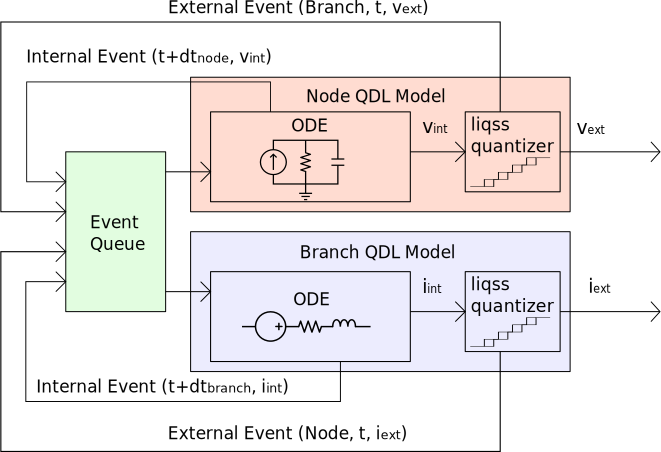
\includegraphics[width=0.6\textwidth]{qdl_sys.png}
    \caption{$2^{nd}$ order QDL system.}
    \label{fig:qdl_sys}
\end{figure}

\begin{figure}[htb]
    \centering
    \includegraphics[width=0.8\textwidth]{qdl_sys_plot.png}
    \caption{$2^{nd}$ order QDL system simulation results (where $v_{dev}$ and $i_{dev}$ are the QDL results, and $v_{ss}$ and $i_{ss}$ are the state-space reference solution results).}
    \label{fig:qdl_sys_plot}
\end{figure}

\section{Distributed Transmission Line}

The next test is a RLCG distributed transmission line model with 5 nodes and 4 branches. The first node includes the external source injection. The results for all of the node voltages ($n1$ through $n5$) and branch currents ($b1$ through $b4$) are shown in figures \ref{fig:qdl_test_9th_voltages} and \ref{fig:qdl_test_9th_currents}. A step change in the source occurs midway through the simulation to provide an additional transient disturbance.

Because the benchmark state space solution and the frequency of updates is an important metric when analyzing the results, the plots contain several types of overlaid information to help visualize these data. First, the reference implicit state space solution results are shown (dashed cyan line). The QDL results are shown as black markers, where each marker is plotted at the time of the atom's external quantized state update. Lastly, the frequency of QDL updates (how often the state is recomputed and an update event is broadcast from the atom) is shown as a histogram of updates per the span of time shown in the plot legend. Note the change in update frequency between the transient and steady-state portions of the simulation.

\begin{figure}[ht]   
    \centering     
    \includegraphics[width=0.95\linewidth]{qdl_test_9th_voltages.png}
    \caption{$9^{th}$ Order Distributed Transmission Line Voltages}     
    \label{fig:qdl_test_9th_voltages}
\end{figure} 


\begin{figure}[ht]   
    \centering     
    \includegraphics[width=0.95\linewidth]{qdl_test_9th_currents.png}
    \caption{$9^{th}$ Order Distributed Transmission Line Currents} 
    \label{fig:qdl_test_9th_currents}
\end{figure} 

\section{Very Stiff Grid Simulation}

In order to test the capabilities of the QDL method with stiff systems, a dense grid was created with a very wide range of time constants. This grid has 16 LIM nodes and 24 LIM branches (see figure \ref{fig:qdl_grid_4x4}). Each quadrant of the grid contains different levels of latency, controlled by setting the capacitance values for the nodes within in the quadrants. The eigenvalues of the system range approximately from $10^{-3}$ seconds to $10^6$ seconds, creating a stiffness ratio of approximately $10^9$. The voltages at the corner nodes are used as representative states for analysis of the results of the simulation, and are conveniently named Node 1, Node 2, Node 3, and Node 4, corresponding to their latency quadrant. 

\begin{figure}[htb]
    \centering
    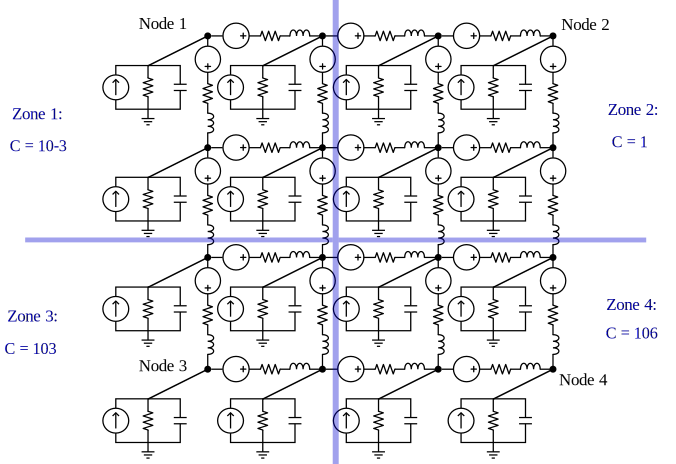
\includegraphics[width=0.9\textwidth]{qdl_grid_4x4.pdf}
    \caption{Stiff LIM grid with four latency zones.}
    \label{fig:qdl_grid_4x4}
\end{figure}   

The simulation was run for $10^4$ simulation seconds. The current injection at Node 1 is stepped from $0$ to $1 A$ at $t=0$, and from $1 A$ to $10 A$ at $t=tsim/2$ to provide a perturbation to create a dynamic response. The results are shown in figure \ref{fig:qdl_stiff_all}. Because the results from a simulation with such a large stiffness ratio are difficult to visualize on one time scale, zoomed plots of the faster transients are included for corner Node 1, Node 2 and Node 3 (see figure \ref{fig:qdl_stiff_zoom_only}). Note that the dynamic response of Node 4 is too slow to warrant a zoomed plot. 

Included in each plot are two axes, a left axis for the voltage quantity, and a right axis for the update frequency. The update frequency is the rate at which the asynchronous state updates occur in the simulation for each atom. As expected and desired, the update frequencies are relatively high during the transients, and very low or non-existent during the steady-state portions. Each plot's legend shows the update frequency histogram bin size in seconds. Note that these bin sizes vary with each plot as they were chosen for readability.  

\begin{figure}[htb]
    \centering
    \includegraphics[width=0.9\textwidth]{qdl_stiff_all.png}
    \caption{Stiff grid corner node voltage dynamic response.}
    \label{fig:qdl_stiff_all}
\end{figure}  

\begin{figure}[htb]
    \centering
    \includegraphics[width=0.9\textwidth]{qdl_stiff_zoom_only.png}
    \caption{Stiff grid corner node voltage dynamic response (zoom to transient).}
    \label{fig:qdl_stiff_zoom_only}
\end{figure} 

An implicit state space solution as a benchmark was impractical to create for this example because of the extreme stiffness and long simulation time of this simulation. The run-time of such a simulation would take many hours or days to simulate on typical desktop hardware using an implicit state space solution with a time step small enough to capture the fast dynamics. For example, a time step of $\lambda_{min}/10$ would require the solution of a 40-state system for $10^8$ time steps. The QDL system, however, requires total updates on the order of $10^5$ for all states combined, and runs in less than 5 mins on a laptop computer as a single-threaded application. Note that this is not an exhaustive performance or accuracy analysis. The quantification of computational efficiency and error will need to be part of future work. Also, because an implicit state space solution is impractical to perform on these types of the extremely stiff systems, a reasonable method of bench-marking the performance and results will have to be determined that does not require running the full simulation.

\section{DC Motor with a PWM Source}

A simulation was performed using QDL for a dc motor excited with a pulse-width modulated voltage source. This system highlights additional features of the QDL method that are not apparent in the previous transmission line or grid models. The DC motor model includes an energy-conversion coupling between the electrical and mechanical sub-networks of the system. This coupling method is very important for the simulation of power systems for the energy transfer in machines, transformers, converters, and loads. The first motor simulation, with results in figure \ref{fig:motor_1} involved a simple dc voltage source armature excitation at startup and shows the resulting armature current and rotor speed. There is an increase in mechanical torque load at the halfway mark. The system is somewhat stiff, with stiffness ratio around 10 between the electric branch and mechanical node (shaft). As expected, very few updates occur in the slower rotor speed state versus the electrical current state, and both atoms update very seldom during the steady-state portions of the simulation. 

\begin{figure}[ht]
    \label{fig:motor_1}
    \centering
    \includegraphics[width=1.0\linewidth]{motor_1.png}
    \caption{DC Motor Simulation}
\end{figure}  

To further test the QDL implementation, the DC motor model was simulated with an ideal PWM source at the armature terminals. Results for the PWM source simulation are shown for small $\Delta Q$ (figure \ref{fig:motor1_pwm_ripple}) as well as large $\Delta Q$ (figure \ref{fig:motor1_pwm_noripple}). In the first case with small $\Delta Q$, there are many updates of the external PWM state (as expected), and also many updates of the external branch current state. The current ripple is recorded in full detail, with updates on the order of 2000 per simulation second. The updates on the rotor speed node are very few and practically non-existent during steady-state. The large $\Delta Q$ simulation demonstrates the ability of QDL to ignore details like PWM-induced ripple while still effectively simulating the system. The $\Delta Q$ is chosen to be larger than the ripple magnitude, which results in the lack of ripple in the output, but more importantly very few updates in the external atom states (total updates are on the order of 10 for each atom).

\begin{figure}[ht]
    \label{fig:motor1_pwm_ripple}
    \centering
    \includegraphics[width=1.0\linewidth]{motor1_pwm_ripple2.png}
    \caption{DC Motor with PWM Source (Small quantum, with ripple)}
\end{figure}  

\begin{figure}[ht]
    \label{fig:motor1_pwm_noripple}
    \centering
    \includegraphics[width=1.0\linewidth]{motor1_pwm_noripple2.png}
    \caption{DC Motor with PWM Source (Large quantum, no ripple)}
\end{figure}  


\chapter{Synchronous Machine Simulation}\label{chap:syncmach}

The purpose of this chapter is to assess the performance of the QDL method to the time-domain simulation of a highly non-linear, complex component of power systems: a three-phase synchronous generator.

In chapter \ref{chap:examples}, a dense, linear network having a very high stiffness ratio ($10^9$) was simulated using a combination of LIQSS1 and latency methods \cite{schutt2001}. The QDL method successfully solved the system response when conventional methods could not (or would have required impractically long simulation times). That work did not address the implications of non-linear system elements. In the previous works surveyed that use QSS integration, the feasibility and performance of QSS-based methods were investigated only for linear systems or for very small non-linear systems (In Di Pietro et al., \cite{pietro2018} for example, a four-stage interleaved converter was simulated using QSS). This chapter attempts to take this a step further by simulating a higher order non-linear power system, specifically with detailed synchronous machine model. 

Systems that include synchronous machines often operate for a long duration in mostly steady-state conditions. These steady conditions are occasionally punctuated by abrupt changes of conditions that must be accurately simulated. The QDL method has the potential for high computational efficiency for simulation of such systems. Non-linearity, high stiffness, and a necessity for algebraic constraints to enforce circuit conservation laws are the important aspects of these systems that we feel QDL is well-suited for.

\section{Study System}

\begin{figure}[h]
    \centering
    \includegraphics[width=0.8\linewidth]{syncmach_schem.png}
    \caption{Synchronous generator connected to an infinite bus.}
    \label{fig:syncmach_schem}
\end{figure}

The study system, shown in figure \ref{fig:syncmach_schem}, has three major components: a prime mover, a synchronous machine (which can act as either a generator or a motor depending on the direction of power flow), and an simple ac power grid model. Models of the prime mover and the grid are simplified. The torque source is an ideal time-dependent source with zero inertia, and the power system is represented as an ideal three-phase sinusoidal ac voltage source with zero impedance and constant frequency (i.e. an infinite bus). This study system was chosen because it is of widespread interest in power systems analysis (the so-called single machine infinite bus, or SMIB system), and because it demonstrates suitability of the QDL method to efficiently solve non-linear systems that are characterized by coupled fast and slow dynamics.

\section{Synchronous Machine Model}

The model of the electric machine is formulated in the synchronous reference frame to eliminate the periodic sinusoidal variations of all voltages and currents via the standard Park transformation \cite{andanapalli2014}. This maximizes the benefit of using the QDL method for the analysis of ac systems, as the potential for slower updates during steady-state conditions relies on flat (zero-derivative) states in steady-state. Although QDL can be used to simulate systems having arbitrary wave forms, the sinusoidal voltage and current oscillations inherent in an ac power system would require rapid state updates that would negate any benefits offered by the QDL method.

\begin{figure}[h]
    \centering
    \includegraphics[width=0.8\linewidth]{syncmach_circuit.png}
    \caption{Direct, quadrature, and mechanical equivalent
        circuits of the synchronous machine.}
    \label{fig:syncmach_circuit}
\end{figure}

A common model of the synchronous generator formulated in the synchronous reference frame is described by the set of equivalent circuits shown in figure \ref{fig:syncmach_circuit}. The fundamental frequency of the study system is 50 Hz. The seventh-order set of nonlinear equations that describe the dynamics of the transformed circuit is described in Equations \ref{eq:sync_mach_diffeq_1} through \ref{eq:sync_mach_diffeq_7}, and the algebraic constraints that apply to the network solution are defined by Equations \ref{eq:sync_mach_alg_1} and \ref{eq:sync_mach_alg_2}. Figure \ref{fig:syncmach_circuit} and the equations follow the model described in \cite{ieee1110}.

\begin{equation}
    \label{eq:sync_mach_diffeq_1}
    \frac{d}{dt} \psi_d = v_d - R_s i_d + \omega_r \psi_q
\end{equation}

\begin{equation}
    \label{eq:sync_mach_diffeq_2}
    \frac{d}{dt} \psi_q = v_q - R_s i_q - \omega_r \psi_d
\end{equation}

\begin{equation}
    \label{eq:sync_mach_diffeq_3}
    \frac{d}{dt} \psi_F = e_{fd} - i_F R_F
\end{equation}

\begin{equation}
    \label{eq:sync_mach_diffeq_4}
    \frac{d}{dt} \psi_D = -i_D R_D
\end{equation}

\begin{equation}
    \label{eq:sync_mach_diffeq_5}
    \frac{d}{dt} \psi_Q = -i_Q R_Q
\end{equation}

\begin{equation}
    \label{eq:sync_mach_diffeq_6}
    \frac{d}{dt} \omega_r = \frac{n}{J} (i_q \psi_d - i_d \psi_q - T_m )
\end{equation}

\begin{equation}
    \label{eq:sync_mach_diffeq_7}
    \frac{d}{dt} \theta = \omega_r - \omega_b
\end{equation}

\begin{equation}
    \label{eq:sync_mach_alg_1}
    \begin{bmatrix}
        i_{dr} \\
        i_F    \\
        i_D
    \end{bmatrix}
    =
    \begin{bmatrix}
        L_{md} + L_{L} & L_{md}         & L_{md}         \\
        L_{md}         & L_{F} + L_{md} & L_{md}         \\
        L_{md}         & L_{F} + L_{md} & L_{F} + L_{md} \\
    \end{bmatrix}^{-1}
    \cdot
    \begin{bmatrix}
        \psi_{dr} \\
        \psi_F    \\
        \psi_D
    \end{bmatrix}
\end{equation}

\begin{equation}
    \label{eq:sync_mach_alg_2}
    \begin{bmatrix}
        i_{qr} \\
        i_Q  
    \end{bmatrix}
    =
    \begin{bmatrix}
        L_{mq} + L_{L} & L_{mq} \\
        L_{mq}         & L_{mq} \\
    \end{bmatrix}^{-1}
    \cdot
    \begin{bmatrix}
        \psi_q \\
        \psi_Q  
    \end{bmatrix}
\end{equation}

Where the terms in these equations are defined as:

\begin{align*}
    \psi_d   & \text{ : direct-axis and stator flux (Wb)}, \\
    \psi_q   & \text{ : quadrature-axis stator flux (Wb)}, \\
    \psi_D   & \text{ : direct-axis damper flux (Wb)}, \\
    \psi_Q   & \text{ : quadrature-axis damper flux (Wb)}, \\
    v_d      & \text{ : direct-axis terminal voltage (V)}, \\
    v_q      & \text{ : quadrature-axis terminal voltage (V)}, \\
    R_s      & \text{ : stator series resistance (} \Omega \text{)}, \\
    \omega_r & \text{ : rotor speed (rad/s)}, \\
    \omega_b & \text{ : base frequency (} 2 \pi 50 \text{ rad/s)}, \\
    i_d      & \text{ : direct-axis stator current (A)}, \\
    i_q      & \text{ : quadrature-axis stator current (A)}, \\
    \psi_F   & \text{ : stator field flux (Wb)}, \\
    i_F      & \text{ : stator field current (A)}, \\
    e_{fd}   & \text{ : field voltage (V)}, \\
    R_F      & \text{ : field resistance (} \Omega \text{)}, \\
    i_D      & \text{ : direct-axis internal equivalent current (A)}, \\
    i_Q      & \text{ : quadrature-axis internal equivalent current (A)}, \\
    R_D      & \text{ : direct-axis equivalent circuit resistance (} \Omega \text{)}, \\
    R_Q      & \text{ : quadrature-axis equivalent circuit resistance (} \Omega \text{)}, \\
    i_{dr}   & \text{ : direct-axis rotor current (A)}, \\
    i_{qr}   & \text{ : quadrature-axis rotor current (A), and}  \\
    \theta   & \text{ : rotor angle relative to synchronous reference frame  (rad).}
\end{align*}


\section{Simulation Scenario and Reference Solution}

The scenario is a typical simulation that initializes the system to steady-state at a specific operating point, and then adds a perturbation to produce a transient response. The simulation starts with the synchronous generator rotating at steady-state in synchronism with the connected grid. This steady-state condition continues for the first $15$ seconds. Beginning at time {t = 15s}, the torque applied by the prime mover to the shaft of the machine begins to ramp up. The torque ramp continues until time {t = 20s}, at which time the torque has reached $25\%$ of the machine’s rated torque. At $25\%$ of rated torque, the phase of the stator voltage leads that of the grid voltage, and the machine drives about $83 MW$ active power and $13 MVAr$ reactive power into the grid.

The system was first simulated using a reference (benchmark) simulation to provide a basis for performance and accuracy comparison of the QDL simulation. The reference solution was obtained by using an implicit Euler integration in MATLAB. A fixed time step of ($10^{-4} s$) was chosen for the Euler solution to ensure stability considering the entire range of eigenvalues. The QDL simulation was obtained by using the LIQSS1 integration method described below.

\section{Implementation of the QDL Model}

The specific QSS integration method used for this example is LIQSS1, described in \cite{pietro2018} and \cite{migoni2009}. The system model comprises seven QDL atom models, one for each of the seven state variables. Figure \ref{fig:syncmach_connect} shows the seven QDL atoms comprising the synchronous machine with directional arrows indicating the external transition graph connections. The system is tightly coupled and components have bidirectional connections. Bi-directional arrows indicate that a state update of either atom requires an update of the other. As an example, following the string of just one arrow, any update to the output of $\psi_{dr}$ requires $\omega_r$ to update the time at which it expects to reach its next quantum level. If the update of $\psi_{dr}$ results in a change of the quantized state of $\omega_r$, then the $\theta$ atom will update the estimate of its transition time to the next quantum transition, and that will feed back to require a next update of $\psi_{dr}$.

To start the solution, the next update time of each atom is initialized to infinity. Each atom then independently computes its own next update time (the time at which it should arrive at its next higher or lower quantum state). The atom with the nearest update time is then updates its external state ($q$) to the appropriate adjacent quantum level. This external state update then flags the connected atoms to update their internal states and next external transition time, and the loop continues. A flowchart of the process is shown in chapter \ref{chap:qdl} figure \ref{fig:qdl_flowchart}.

\begin{figure}[h]
    \centering
    \includegraphics[width=0.8\linewidth]{syncmach_connect.png}
    \caption{Synchronous machine model QDL atoms showing the external state transition connections.}
    \label{fig:syncmach_connect}
\end{figure}

\section{QDL Performance}

The performance of the QDL method is shown in comparison to the performance of the reference solution in a series of plots. Each plot shows the trajectory of a state variable and the cumulative number of updates (or re-evaluations) of the QDL atom for that state variable. All states in the system use the same quantization step size ($\Delta Q$) of $10^{-4} Wb$, except the machine rotor speed ($\omega_r$) for which we choose a $\Delta Q$ $1/10^{th}$ as large as the others ($10^{-5} rad/s$) since the dynamic range of the rotor speed is much less than that of the system fluxes. For simplicity, this simulation does not use a complex methodology for choosing the best $\Delta Q$. A $\Delta Q$ of roughly 0.1\% of the total expected deviation (the absolute value of the dynamic range of the quantity in the reference simulation) of the quantized state variable. Another objective of the this simulation is to investigate the relationship between $\Delta Q$ and solution error. Understanding this relationship could lead to a more rigorous methodology for choosing $\Delta Q$ based on a desired error bound. Figures \ref{fig:syncmach_fdr}, \ref{fig:syncmach_fqr} and \ref{fig:syncmach_fF} show the accuracy with which the QDL method tracks the reference solution. The cumulative number of updates for a particular atom is shown by the red lines in the following charts, with each state's cumulative updates being unique. Further discussion on the relationship between $\Delta Q$ and error, and alternative methods for $\Delta Q$ selection can be found in chapter \ref{chap:deltaq}.

An performance advantage of the QDL method over the reference solution can be seen as the system reaches the new steady state condition and the rate of atom updates markedly decreases. For example, in figure \ref{fig:syncmach_fdr}, during the interval from 0 to 15 seconds, while the system is in steady-state, there are very few state updates. During the period from 15 sec to 35 seconds, however, while the machine is accelerating (and the other states of the system are rapidly changing), the slope of the curve representing the cumulative number of updates is large. Finally, after around 35 seconds, the system approaches a new steady-state and the update rate decreases. This aspect of the QDL method allows the simulation to advance rapidly during steady-state conditions, and speed up again when fast transient behavior requires more time resolution. Also, the cumulative number of updates depends on the chosen $\Delta Q$. In general, a smaller $\Delta Q$ will tend to require more frequent updates, and the simulation will tend to advance more slowly through time. However, it is important to note that the effects of changing the $\Delta Q$ on performance and accuracy is complex, and warrants further discussion and investigation (see chapter \ref{chap:deltaq}).

\begin{figure}[h]
    \centering
    \includegraphics[width=0.8\linewidth]{syncmach_fdr.png}
    \caption{Rotor d-axis flux. The flux computed by the QDL method is nearly identical to that computed by the reference method so the two lines are nearly indistinguishable. Cumulative count of $\psi_{dr}$ atom updates shows little activity prior to torque ramp, higher activity during torque ramp, and a return to little activity as new steady state is attained.}
    \label{fig:syncmach_fdr}
\end{figure}

\begin{figure}[h]
    \centering
    \includegraphics[width=0.8\linewidth]{syncmach_fqr.png}
    \caption{Rotor q-axis flux. The values computed by the QDL method and the reference method are nearly indistinguishable.}
    \label{fig:syncmach_fqr}
\end{figure}

\begin{figure}[h]
    \centering
    \includegraphics[width=0.8\linewidth]{syncmach_fF.png}
    \caption{Field flux, showing good agreement between both computing methods and a total number of QDL atom updates that is smaller than the counts for d- and q-axis fluxes.}
    \label{fig:syncmach_fF}
\end{figure}

\begin{figure}[h]
    \centering
    \includegraphics[width=0.8\linewidth]{syncmach_theta.png}
    \caption{Rotor angle. QDL update rate shows interesting behavior with faster rates associated with beginning and ending of the torque ramp.}
    \label{fig:syncmach_theta}
\end{figure}

The trajectory of rotor angle ($\theta$) , as shown in figure \ref{fig:syncmach_theta}, is particularly interesting in that it shows how the count of this atom’s updates increases immediately after the start of the torque ramp-up, then tapers off while the torque slew rate is constant during the interval between 15 to 20 seconds, then increases again at 20 seconds when the torque stops moving, and finally becomes small again as the rotor angle reaches its final steady state value. Figure \ref{fig:syncmach_wr} shows the trajectory of the rotor speed which always remains very close to 100 rad/s, but shows structure near the beginning and ending of the torque ramp, and a small speed increase during the torque ramp-up.

\begin{figure}[h]
    \centering
    \includegraphics[width=0.8\linewidth]{syncmach_wr.png}
    \caption{Rotor speed trajectory and update rates.}
    \label{fig:syncmach_wr}
\end{figure}

\begin{figure}[h]
    \centering
    \includegraphics[width=0.8\linewidth]{syncmach_current.png}
    \caption{Comparisons of d- and q-axis rotor currents computed by the QDL and reference solutions.}
    \label{fig:syncmach_current}
\end{figure}

\begin{figure}[h]
    \centering
    \includegraphics[width=0.8\linewidth]{syncmach_voltage.png}
    \caption{Comparisons of d- and q-axis voltages computed by the QDL and reference solutions.}
    \label{fig:syncmach_voltage}
\end{figure}

\section{Accuracy and Error Analysis}

In \cite{kofman2001b}, the authors proved that, for linear time-invariant systems, the global error in QSS integration solutions can be bounded by a constant proportional to the quantization step size ($\Delta Q$). However, our reference system is highly non-linear, so it is interesting to explore the behavior of error with varying $\Delta Q$. 
The effect $\Delta Q$ on simulation accuracy is shown in figures \ref{fig:syncmach_wr_qstep}, \ref{fig:syncmach_wr_qstep_ZOOM} and \ref{fig:syncmach_wr_qstep_ZOOM2}, where several system variables are plotted for a range of $\Delta Q$ values, with enhanced detail during particular time periods.  A larger quantization step  size results in both a lower update rate and a higher error amplitude compared to a situation with a smaller $\Delta Q$. In each case, the quoted $\Delta Q$ applies to all of the state variables except rotor speed, for which the quantization step is $1/10^{th}$ that of the other variables. In each plot, the trajectory with green color corresponds to the largest $\Delta Q$ of $10^{-3}$, while blue and red correspond to smaller sizes ($\Delta Q = 10^{-4}$  and $\Delta Q = 10^{-5}$ respectively). The rotor speed calculated with the largest $\Delta Q$ has the largest error in comparison to the reference solution. This is evident in both figure \ref{fig:syncmach_wr_qstep_ZOOM}, in which resolution is increased near the apex of the speed trajectory, and in figure \ref{fig:syncmach_wr_qstep_ZOOM2} where higher resolution shows a slightly oscillating speed trajectory after the torque ramp. These high frequency oscillations are inherent to the QDL method and the amplitude of these oscillations increases as the $\Delta Q$ increases. The sensitivity data provided in this chapter have been empirically determined from simulation of this specific system with specific component parameters. Although this empirical data does provide useful insight into the relationship between $\Delta Q$ and error, it does not solve the problem for the general case.

\begin{figure}[h]
    \centering
    \includegraphics[width=0.8\linewidth]{syncmach_wr_qstep.png}
    \caption{Rotor speed using different quantization sizes ($\Delta Q = 10^{-5}$, $\Delta Q = 10^{-4}$, $\Delta Q = 10^{-5}$ vs Euler method reference solution.}
    \label{fig:syncmach_wr_qstep}
\end{figure}

\begin{figure}[h]
    \centering
    \includegraphics[width=0.8\linewidth]{syncmach_wr_qstep_ZOOM.png}
    \caption{Zoom plots from 18 sec to 18.5 sec of rotor speed using different quantization sizes $\Delta Q = 10^{-5}$, $\Delta Q = 10^{-4}$, $\Delta Q = 10^{-3}$ vs Euler method reference solution.}
    \label{fig:syncmach_wr_qstep_ZOOM}
\end{figure}

\begin{figure}[h]
    \centering
    \includegraphics[width=0.8\linewidth]{syncmach_wr_qstep_ZOOM2.png}
    \caption{Zoom-in plots that show details for steady state situation of rotor speed using different quantization sizes $\Delta Q = 10^{-5}$, $\Delta Q = 10^{-4}$, $\Delta Q = 10^{-5}$ vs Euler reference solution. The oscillations have very small amplitudes.}
    \label{fig:syncmach_wr_qstep_ZOOM2}
\end{figure}

Figures \ref{fig:syncmach_wr_error_time} and \ref{fig:syncmach_wr_error_qstep} describe the same behavior as was shown in figures \ref{fig:syncmach_wr_qstep}, \ref{fig:syncmach_wr_qstep_ZOOM}, and \ref{fig:syncmach_wr_qstep_ZOOM2} but from the error perspective. Figure \ref{fig:syncmach_wr_error_time} shows how the point-wise absolute error (the difference between the QDL simulation and the reference simulation) varies over a particular half-second interval. The time variation of error in the state variable $\psi_{dr}$ is shown for several different $\Delta Q$ ranging from $\Delta Q = 10^{-6}$ to $\Delta Q = 10^{-2}$. Clearly, a larger $\Delta Q$ produces a larger error in this case, but the relationship was not linear. Before the torque ramps up, the different $\Delta Q$ values all produce negligible errors. After the torque starts to ramp up, the number of updates starts to grow and the models using larger quantization sizes produce larger errors. Although a small quantization size improves the simulation accuracy, it also causes a larger model update rate. Therefore, if computing speed is important, and if a larger percent error is tolerable, one might choose a large $\Delta Q$ in order to achieve the requisite computing speed.

\begin{figure}[h]
    \centering
    \includegraphics[width=0.8\linewidth]{syncmach_wr_error_time.png}
    \caption{Error between reference solution and QDL solution of rotor d-axis flux for several different quantization sizes $\Delta Q = 10^{-2}$ , $\Delta Q = 8.86\cdot 10^{-4}$, $\Delta Q = 10^{-6}$.}
    \label{fig:syncmach_wr_error_time}
\end{figure} 

To generate the data shown in figure \ref{fig:syncmach_wr_error_qstep} we quantized the rotor speed at $\Delta Q = 10^{-7}$ and the other state variables at $\Delta Q = 10^{-4}$. This was an experiment to see if choosing a relatively small quantization size for some particular interesting state, but leaving other quanta larger, would produce fewer updates for the whole system, while still having a small error for the particular state of interest. Figure \ref{fig:syncmach_wr_error_qstep} shows that the state of rotor speed experienced a high number of updates, but the error did not reduce compared to the simulation with system-wide $\Delta Q = 10^{-4}$, which produced the same output with a smaller number of updates. 

\begin{figure}[h]
    \centering
    \includegraphics[width=0.8\linewidth]{syncmach_wr_error_qstep.png}
    \caption{Rotor speed updates vs relative error when rotor speed $\Delta Q$ is set to $10^{-7}$  and the quantization size of the rest of the system variables is $\Delta Q = 10^{-4}$. Possibly unnecessary high precision with low benefit of error reduction}
    \label{fig:syncmach_wr_error_qstep}
\end{figure} 

Figure \ref{fig:syncmach_error_qstep_all} shows the maximum error among any system variable at any time during the simulation interval. The graph is plotted on a logarithmic scale as a function of the $\Delta Q$, which was varied from $10^{-6}$ to $10^{-2}$ Wb. Also plotted is the corresponding sum of all updates of all atoms over the entire simulation. For small $\Delta Q$ values of $10^{-6}$ to $10^{-5}$ Wb, the error is very small and largely independent of $\Delta Q$. A logarithmic scale is used to emphasize that for very small $\Delta Q$ values ($10^{-5}$ Wb), a decrease in $\Delta Q$ does not improve the accuracy, but it does impose a penalty on computational intensity (simulation update rate), and the simulation takes longer to advance through time with no- significant error reduction. A sweet spot is evident around $\Delta Q$ between $10^{-5}$  to $10^{-4}$, where computational intensity has become relatively low while error also remains low. Above $\Delta Q$ values of around $10^{-4}$, the error increases rapidly, but without a consistent reductions in computational intensity.

\begin{figure}[h]
    \centering
    \includegraphics[width=0.8\linewidth]{syncmach_error_qstep_all.png}
    \caption{Maximum Error of all atoms for different $\Delta Q$ values. Total number of the updates decreases as the system is simulated with bigger $\Delta Q$ values at the expense of increasing the error.}
    \label{fig:syncmach_error_qstep_all}
\end{figure} 

Although the QDL method does accurately track the reference solution, the method does inherently exhibit steady-state oscillations. These oscillations are evident in figure \ref{fig:syncmach_fdr_ripple}, which shows the direct axis rotor flux at high resolution just near the onset of the torque ramp at 15 seconds. The amplitudes of these high frequency oscillations reduce as the $\Delta Q$ is reduced, but the oscillations are always present. Each oscillation represents an update event, so reducing the oscillation size comes at the expense of computation time. Figures \ref{fig:syncmach_fdr_ripple} and \ref{fig:syncmach_fdr_transient} show these high frequency oscillations at $\Delta Q$ values of $10^{-4}$  and $10^{-5}$. The mitigation of this high-frequency oscillation behavior is discussed further in chapter \ref{chap:steadystate}. 

\begin{figure}[h]
    \centering
    \includegraphics[width=0.8\linewidth]{syncmach_fdr_ripple.png}
    \caption{High resolution plot showing the ripples in QDL solution of the rotor d-axis flux $\psi_{dr}$ with $\Delta Q$ of $10^{-4}$.}
    \label{fig:syncmach_fdr_ripple}
\end{figure}

\begin{figure}[h]
    \centering
    \includegraphics[width=0.8\linewidth]{syncmach_fdr_transient.png}
    \caption{High resolution plot showing the ripples in the QDL solution of the rotor d-axis flux $\psi_{dr}$ with $\Delta Q$ of $10^{-5}$. The amplitude of the ripples is smaller compared to $\Delta Q$ of $10^{-4}$.}
    \label{fig:syncmach_fdr_transient}
\end{figure}

\section{Study Summary}

The performance of the QDL method for analyzing the dynamics of non-linear power system that includes a detailed synchronous machine model has been investigated. Uniform quantization of system state variables at 0.01 percent was found to yield accuracy within 0.4 percent of that achieved with a conventional implicit state-space solution, but with a significant advantage in computational intensity, especially for systems that operate for long times in a quasi-steady-state. Since the QDL method enables the user to individually set the quantization step size ($\Delta Q$) values of each state, we evaluated performance as a function of $\Delta Q$. When the system was simulated using one uniform quantization size for all states, the total number of state updates generally decreased as $\Delta Q$ increased, but above a quantization size of about $10^{-4}$, further increase in $\Delta Q$ did not significantly reduce the computational cost (but it did decrease the simulation accuracy). When $\Delta Q$ for a single state of interest was set smaller than the uniform $\Delta Q$ of other states, refining the $\Delta Q$ of that particular state variable did not necessarily improve the error of that particular state, but it did logarithmically increase the state update intensity of the whole system. The observations of the effects of $\Delta Q$ selection are limited by the particular system that was studied. Other systems, especially those having state variables that are widely different in magnitude, may behave differently.



\chapter{Power System Simulation}\label{chap:powersys}

The purpose of this chapter is to test the feasibility and performance of the QDL method for the modeling and simulation of the dynamic performance of a relatively large and realistic power system model. The system model created for this evaluation is a three-phase network consisting of a synchronous machine, a turbine, a governor, an exciter, an induction motor, an ac/dc converter, a dc load, and a constant impedance load. All of these devices are connected through a three-phase network consisting of several buses and transmission lines. This study system contains a high range of transient behavior, from the slow mechanical transients of the rotating machines, to the very fast transients of the electrical quantities on the network. This is therefore mathematically a very stiff system model, which poses a challenge of effectively simulating the system over significant periods of simulation time while capturing the full range of transient behavior using a single representation of the power system. Because the QDL approach primarily quantizes the simulation states (and not time), it should therefore be well-suited to the task of simulating the slow and fast dynamics of system without some of the numerical stability and efficiency issues inherent in solving stiff systems using traditional time-slicing methods. 

The benefits of QDL methods are best leveraged by systems whose states have derivatives that approach zero at steady-state. A ac power system that has sinusoidal steady-state behavior in the stationary reference frame is therefore best modeled in the rotating reference frame using a Park transformation. The QDL method than then take advantage of the benefits of the QDL steady-state performance behavior. The variable time spans between state updates should be longer during steady-state conditions without sacrificing accuracy during the fast transients.

\section{System Model}

\begin{figure}[h]
    \label{fig:powersys}
    \centering
    \includegraphics[width=0.8\linewidth]{powersys.png}
    \caption{Power system schematic}
\end{figure}

The reference system is a three-phase, 60 Hz, 4160 V (line-line RMS) power system consisting of a synchronous machine being operated as a generator, connected to three loads via a network of buses and cables. An induction motor is connected to bus two and the other two loads, a dc load behind a converter and a constant impedance (RL) load are connected to bus three. The converter is represented as a non-linear dq averaged model. The cables are represented using a standard pi model. With 32 states, this power system is designed to be simple enough for the testing of a novel simulation method, while complex enough to represent a realistic, non-linear power system. For each device, a model was QDL compliant device model was formulated. These models are described in the next section.

The descriptions for each of the device models for the study system are given below, along with the derivation of the QDL model.

\section{Cable Model}

\begin{figure}[h]
    \label{fig:powersys_cable}
    \centering
    \includegraphics[width=0.75\linewidth]{powersys_cable.png}
    \caption{Cable model}
\end{figure}

Each cable is represented as a lumped pi model of a transmission line as described in \cite{gholizadeh2021}. The equivalent circuit is shown in figure \ref{fig:powersys_cable}. Note that only the q-axis model is shown. The d-axis portion of model and is identical to q-axis portion, except the voltage and current quantities are their d-axis counterparts. This model differs from the cable model in \cite{gholizadeh2021}, in that the shunt conductance and capacitance elements have been added to the ends of the branch in order to provide full latency required by the QDL and simulation method. This model provides full branch and node latency by exploiting the inherit latency from the physical branch inductance and the node capacitance. The dynamic equations that describe the cable model are 

\begin{equation} \label{eq:cable_iq}
\frac{d}{dt}i_{q}=\frac{-(R+\omega L)i_{q}+(v_{q1}-v_{q2})}{L}    
\end{equation}

\begin{equation} \label{eq:cable_vq1}
    \frac{d}{dt}v_{q1}=\frac{-(\frac{G+\omega C}{2})v_{q1}+\sum{i_{branch}}}{C/2}    
\end{equation}

Where all quantities are those represented in figure \ref{fig:powersys_cable}, and $\sum{i_{branch}}$ is the sum of all currents injected from all branches connected to node $v_{q1}$. Similar equations are used for the other states $v_{q2}$, $v_{d1}$, $v_{d2}$ and $i_d$.

To construct the system model, the LIM node conductance and capacitance quantities are summed together automatically with other devices connected to the same bus. In other words, each bus's LIM node model is created by combining the contributions from the terminals of all connected devices with shunt conductance and capacitance elements. 

\section{RL Load Model}

The RL Load is modeled as dq series impedance branches connected to ground. The equivalent circuit is shown in figure \ref{fig:powersys_load} 

\begin{figure}[h]
    \label{fig:powersys_load}
    \centering
    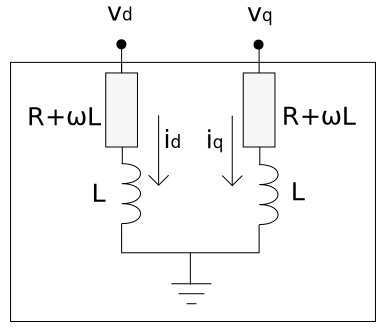
\includegraphics[width=0.5\linewidth]{powersys_load.png}
    \caption{RL Load}
\end{figure}  

Because this model is fully described by LIM atoms, the equations are not given here (see the LIM node atom description in chapter \ref{chap:lim}, figure \ref{fig:lim_dependent_node}).

\section{Transformer-Rectifier Model}

\begin{figure}[h]
    \label{fig:powersys_trload}
    \centering
    \includegraphics[width=0.95\linewidth]{powersys_trload.png}
    \caption{Transformer-Rectifier Load}
\end{figure} 

The Transformer-rectifier load model is based on the model found in \cite{abdelwahed2013}, and includes a non-linear coupling between d and q-axis constant current branches and a dc side with a LIM branch and node. The equivalent circuit model is shown in figure \ref{fig:powersys_trload}. The ac-dc coupling is defined by

\begin{equation} \label{eq:trload_igd}
    i_{gd}=S_{d}i_{dc}   
\end{equation}

\begin{equation} \label{eq:trload_igq}
    i_{gq}=S_{q}i_{dc}   
\end{equation}

\begin{equation} \label{eq:trload_vg}
    v_{g} = \frac{v_{d}}{S_{d}} + \frac{v_{q}}{S_{q}}   
\end{equation}

where the coupling coefficients are

\begin{equation} \label{eq:trload_sd}
    S_{d} = 2 \sqrt{\frac{2}{3}} \frac{\sqrt{3}}{\pi} \cos{\phi}    
\end{equation}

\begin{equation} \label{eq:trload_sq}
    S_{q} = -2 \sqrt{\frac{2}{3}} \frac{\sqrt{3}}{\pi} \sin{\phi}.    
\end{equation}

where $\phi$ is the firing angle. The dc subsystem of this model is a LIM branch, the equations for which are given in chapter \ref{chap:lim}, figure \ref{fig:lim_dependent_branch}.

\section{Synchronous Machine}

The synchronous machine \cite{abdelwahed2013} is modeled at two LIM branches for the electrical model (one for each dq axis), and a LIM node for the mechanical dynamics. The equivalent circuit is shown in figure \ref{fig:powersys_sm}

\begin{figure}[h]
    \label{fig:powersys_sm}
    \centering
    \includegraphics[width=0.95\linewidth]{powersys_sm.png}
    \caption{Synchronous Machine}
\end{figure}

The electro-mechanical dynamics are modeled with the flux differential equations

\begin{equation}
\frac{d}{dt} \psi_{kq} = \frac{r_{kq}}{L_{lkq}} \left( \psi_{kq} - L_{q} i_{qs} - \psi_{q} i_{qs}+L_{ls} i_{qs} \right)
\end{equation}

\begin{equation}
    \frac{d}{dt} \psi_{kd} = \frac{r_{kd}}{L_{lkd}} \left( \psi_{kd} - L_{d} i_{ds} - \psi_{d} i_{ds}+L_{ls} i_{ds} \right)
\end{equation}

\begin{equation}
    \frac{d}{dt} \psi_{fd} = \frac{r_{fd}}{L_{lfdd}} \left( \psi_{fd} - L_{d} i_{ds} - \psi_{d} i_{ds}+L_{ls} i_{ds} - v_{fd} \right)
\end{equation}

where the electrical torque $T_e$ is coupled to the terminal currents $i_{qs}$, $i_{ds}$ as

\begin{equation}
    T_e = \frac{3P}{4} \left( \psi_{ds} i_{qs} - \psi_{qs} i_{ds} \right)
\end{equation}

and the q- and d-axis equivalent fluxes and inductances are given by

\begin{equation}
    L_q = L_{ls} + \frac{L_{mq}L_{lkq}}{L_{lkq} + L_{mq}}
\end{equation}

\begin{equation}
    L_d = L_{ls} + \frac{L_{md} L_{lfd} L_{lkd}}{L_{md} L_{lfd} + L_{md} L_{lkd} + L_{lfd} L_{lkd}}
\end{equation}

\begin{equation}
    \psi_q = \frac{L_{mq}}{L_{mq} + L_{kd}} \psi_kd
\end{equation}

\begin{equation}
    \psi_d = \frac{L_{md} \left( \frac{\psi_{kd}}{L_{lkd}} + \frac{\psi_{fd}}{L_{lfd}} \right) }{1 + \frac{L_{md}}{L_{lfd}} + \frac{L_{md}}{L_{lkd}}}
\end{equation}.

\section{Turbo-Governor Model}

The dynamics of the prime mover and the speed governor are combined into a single model described by

\begin{equation}
    T_m = K_p \delta_r + K_i \theta_r
\end{equation}

where $T_m$ in the mechanical torque, $K_p$ and $K_i$ are the PI controller constants, and the speed deviation $\delta_r$ and rotor angle $\theta_r$ are related to the synchronous speed ($\omega_s$) and the machine rotor speed ($\omega_r$) as

\begin{equation}
    \delta_r = \omega_s - \omega_r
\end{equation}

\begin{equation}
    \frac{d}{dt} \theta = \delta_r.
\end{equation}.

\section{Exciter Model}

The synchronous machine terminal voltage is regulated using an exciter. The exciter model used is a simplified IEEE AC8B Exciter model. This is modeled as four differential equations for three internal signal states as well as the output voltage. 

The input is the per unit terminal voltage magnitude, and the output is the per unit field voltage $v_{fd}$. The differential equations are 

\begin{equation}
    \frac{d}{dt} x_1 = v_{term,pu} - \frac{1}{T_{dr}} x_1
\end{equation}

\begin{equation}
    \frac{d}{dt} x_2 = x_1
\end{equation}

\begin{equation}
    \frac{d}{dt} x_3 = \left( K_{ir} - \frac{K_{dr}}{T^2_{dr}} \right) x_1
    + \frac{K_{ir}}{T_{dr}} x_2 - \frac{1}{T_a} x_3
    + \left( \frac{K_{dr}}{T_{dr}} + K_{pr} \right) v_{term,pu}
\end{equation}

\begin{equation}
    \frac{d}{dt} v_{fd,pu} = \frac{K_a}{T_a T_e} x_3 - \frac{K_e}{T_e} v_{fd,pu}
\end{equation}

where the per unit terminal voltage $v_{t,pu}$ is related to the machine dq quantities and the rated line-line terminal voltage magnitude $V_{base,LL}$ as

\begin{equation}
    v_{term,pu} = \frac{\sqrt{v^2_{qs} + v^2_{ds}}}{V_{base,LL}}
\end{equation}

and the per unit output of the exciter $v_{fd,pu}$ is then scaled by the base voltage $V_{base,LL}$ before being input into to synchronous machine model as

\begin{equation}
    v_{fd} = v_{fd,pu} \cdot V_{base,LL}
\end{equation}.

\section{Induction Machine Model}

The induction machine is modeled as two LIM branches for the electrical model (one for each dq axis) and a LIM node for the mechanical dynamics as shown in figure \ref{fig:powersys_im}

\begin{figure}[h]
    \label{fig:powersys_im}
    \centering
    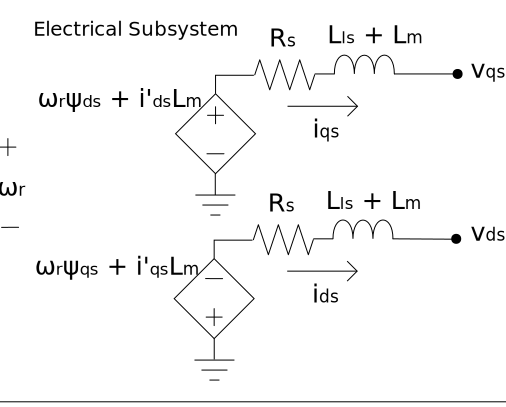
\includegraphics[width=0.95\linewidth]{powersys_im.png}
    \caption{Induction Machine}
\end{figure}

The LIM sources are updated using the flux quantities defined in terms of the instantaneous stator and rotor d- and q- access currents using

\begin{equation}
    \psi_{qs} = L_{ls} i_{qs} + l_m (i_{qs} + i_{qr} )
\end{equation}

\begin{equation}
    \psi_{ds} = L_{ls} i_{ds} + l_m (i_{ds} + i_{dr} )
\end{equation}

\begin{equation}
    \psi_{qr} = L_{lr} i_{qr} + l_m (i_{qr} + i_{qs} )
\end{equation}

\begin{equation}
    \psi_{dr} = L_{lr} i_{dr} + l_m (i_{dr} + i_{ds} )
\end{equation},

And the mechanical dynamics are resolved using the LIM node model in figure \ref{fig:powersys_im}, where the electrical torque $T_e$ is determined from the currents using

\begin{equation}
    T_e = \frac{P}{2J} \left(
    \frac{3P}{4} \left( L_{ls} i_{ds} + L_m
    \left( i_{ds} + i_{dr} \right)\right)
    i_{qs} - \left(L_{ls} i_{qs} + L_m
    \left(i_{qs} + i_{qr} \right)\right)
    i_{ds}-T_b \left( \frac{\omega_r}{\omega_s}
    \right)^3 \right)
\end{equation}

where $P$ is the number of pole pairs, $T_b$ is the base torque, and $\omega_s$ and $\omega_r$ are the synchronous and rotor speeds respectively. 

\section{Simulation Scenario and Benchmark Solution}

In the simulation scenario, the system starts in steady-state (all state derivatives are zero), using a standard iterative ODE operating point solution. At time $t=0$ seconds, the active power of RL load is increased by 20\%. A reference solution (denoted "ODE" in the output plots) is run with identical parameters and events to compare the results and quantify error. 

In order to provide results for performing accuracy and performance bench-marking, a traditional integration method was used that is well-suited to non-linear, stiff systems. The modeling method used to benchmark accuracy  and performance uses a representation of the system as a set of non-linear, first order differential equations. The QDL formulation of the power system provides a full state-space description of the system, including the system Jacobian matrix that can be used directly with many numerical integration techniques. The integration method used to compute the benchmark is an implicit Runge-Kutta method of the Radau IIA family of order 5, a method well-suited for these types of stiff systems. The fixed time step was chosen to be $10 \mu s$ to easily accommodate the fastest eigenvalues of the system.

\section{Simulation Results}

Each plot presented for the simulation results includes the QDL results as the solid color curves, the benchmark results as a dashed gray curve, and the cumulative atom updates as a dashed color curve with a separated $y$ axis on the right. Each plotted atoms' results are shown for the entire 60 seconds of simulation, along with zoom plots to the transient around the disturbance at 1 second simulation time. The time range of each zoom plot is chosen to highlight the performance of QDL for the specific dynamic behavior for that specific state, as some states move much faster than others. Some plots included filtered results to reduce spurious noise as discussed in section \ref{sec:filtering}.

\begin{figure}[h]
    \centering
    \includegraphics[width=0.95\linewidth]{powersys_plot_loadinc_sm_wr.png}
    \caption{Synchronous machine speed.}
    \label{fig:powersys_plot_loadinc_sm_wr}
\end{figure}

\begin{figure}[h]
    \centering
    \includegraphics[width=0.95\linewidth]{powersys_plot_loadinc_sm_wr_ZOOM.png}
    \caption{Synchronous machine speed, zoom to transient.}
    \label{fig:powersys_plot_loadinc_sm_wr_ZOOM}
\end{figure}

\begin{figure}[h]
    \centering
    \includegraphics[width=0.95\linewidth]{powersys_plot_loadinc_sm_iqs.png}
    \caption{Synchronous machine q-axis stator current (filtered, $fc=100 Hz$).}
    \label{fig:powersys_plot_loadinc_sm_iqs}
\end{figure}

\begin{figure}[h]
    \centering
    \includegraphics[width=0.95\linewidth]{powersys_plot_loadinc_sm_iqs_ZOOM.png}
    \caption{Synchronous machine q-axis stator current, zoom to transient (filtered, $fc=100 Hz$)}
    \label{fig:powersys_plot_loadinc_sm_iqs_ZOOM}
\end{figure}

\begin{figure}[h]
    \centering
    \includegraphics[width=0.95\linewidth]{powersys_plot_loadinc_rlload.png}
    \caption{RL Load currents.}
    \label{fig:powersys_plot_loadinc_rlload}
\end{figure}

\begin{figure}[h]
    \centering
    \includegraphics[width=0.95\linewidth]{powersys_plot_loadinc_rlload_ZOOM.png}
    \caption{RL Load currents, zoom to transient.}
    \label{fig:powersys_plot_loadinc_rlload_ZOOM}
\end{figure}

\begin{figure}[h]
    \centering
    \includegraphics[width=0.95\linewidth]{powersys_plot_loadinc_trload.png}
    \caption{Transformer-rectifier load d-axis current and dc voltage.}
    \label{fig:powersys_plot_loadinc_trload}
\end{figure}

\begin{figure}[h]
    \centering
    \includegraphics[width=0.95\linewidth]{powersys_plot_loadinc_trload_ZOOM.png}
    \caption{Transformer-rectifier load d-axis current and dc voltage, zoom to transient.}
    \label{fig:powersys_plot_loadinc_trload_ZOOM}
\end{figure}

\begin{figure}[h]
    \centering
    \includegraphics[width=0.95\linewidth]{powersys_plot_loadinc_bus1_vd.png}
    \caption{Bus 1 d-axis voltage.}
    \label{fig:powersys_plot_loadinc_bus1_vd}
\end{figure}

\begin{figure}[h]
    \centering
    \includegraphics[width=0.95\linewidth]{powersys_plot_loadinc_bus1_vd_ZOOM.png}
    \caption{Bus 1 d-axis voltage, zoom to transient.}
    \label{fig:powersys_plot_loadinc_bus1_vd_ZOOM}
\end{figure}

\begin{figure}[h]
    \centering
    \includegraphics[width=0.95\linewidth]{powersys_plot_loadinc_im_wr.png}
    \caption{Induction machine speed.}
    \label{fig:powersys_plot_loadinc_im_wr}
\end{figure}

\begin{figure}[h]
    \centering
    \includegraphics[width=0.95\linewidth]{powersys_plot_loadinc_im_wr_ZOOM.png}
    \caption{Induction machine speed, zoom to transient.}
    \label{fig:powersys_plot_loadinc_im_wr_ZOOM}
\end{figure}

\begin{figure}[h]
    \centering
    \includegraphics[width=0.95\linewidth]{powersys_plot_loadinc_cable23_100hz.png}
    \caption{Cable currents from bus 2 to bus 3 q-axis (filtered, $f_c=100 Hz$).}
    \label{fig:powersys_plot_loadinc_cable23_100hz}
\end{figure}

\begin{figure}[h]
    \centering
    \includegraphics[width=0.95\linewidth]{powersys_plot_loadinc_cable23_ZOOM_100hz.png}
    \caption{Cable currents from bus 2 to bus 3 q-axis, zoom to transient (filtered, $f_c=100 Hz$).}
    \label{fig:powersys_plot_loadinc_cable23_ZOOM_100hz}
\end{figure}

From inspection of the plots in figures \ref{fig:powersys_plot_loadinc_sm_wr} to \ref{fig:powersys_plot_loadinc_cable23_ZOOM_100hz}, the transient behavior of all states tracts the benchmark solution very well. The steady-state behavior, although bounded, shows significant oscillations. This highlights the importance of the topics discussed in chapter \ref{chap:steadystate} for detecting steady-state, and filtering spurious oscillations from the results using post-simulation filtering.  
 
\section{Error Analysis}

Error was quantified using the normalized RMS deviation calculation defined as

\begin{equation}
    \text{NRMSD} = \frac{ \sqrt{ \frac{\sum_{i=1}^N{(y_i - q_i)^2}}{N} } }{\max{y} - \min{y}}.
\end{equation}

where $y_i$ is the benchmark (ODE) solution result for the state variable at point i, $q_i$ is the quantized QDL solution result for the state variable at point i, $N$ is the number of solution points, and the quantity $\max{y} - \min{y}$ is the dynamic range of the variable in the benchmark simulation. 
    
This method of producing aggregated error values was chosen in order to provide error results that could be meaningfully compared across the states of the simulation, given the vastly different offsets and dynamic ranges between the states. The errors observed for the load increase simulation are shown in the sorted bar chart in figure \ref{fig:powersys_plot_error}.

\begin{figure}[h]
    \centering
    \includegraphics[width=0.95\linewidth]{powersys_plot_error.png}
    \caption{Simulation NRMSD error by state variable}
    \label{fig:powersys_plot_error}
\end{figure}

The q-axis current on the cable from bus 2 to 3 is the state with the highest aggregated error in the simulation. This is not surprising given the level of high-amplitude noise seen in the simulation output for this variable. See chapter \ref{chap:steadystate} for further discussion on post-process filtering of these data to improve readability of results, and to reduce error.

\section{Performance Analysis}

To analyze the performance of the QDL method for this system, a proxy for computation intensity was used to estimate the relative performance of the QDL method against the benchmark ODE solution. This proxy is the cumulative number of updates for each atom. Although not directly comparable to time-slicing method time step counts, it gives us a good approximation of the relative computational efficiency of the QDL method vs. the reference ODE solution. Note that, in order to produce a stable simulation, a time step of $10\mu s$ was used, which results in $6 \times 10^{5}$ time steps for a 60 second (simulation time) simulation.  

\begin{figure}[h]
    \centering
    \includegraphics[width=0.75\linewidth]{powersys_vref_inc_updates_60s_sm.png}
    \caption{Cumulative QDL atom updates vs. simulation time, synchronous machine states}
    \label{fig:powersys_vref_inc_updates_60s_sm}
\end{figure} 

\begin{figure}[h]
    \centering
    \includegraphics[width=0.75\linewidth]{powersys_vref_inc_updates_60s_im.png}
    \caption{Cumulative QDL atom updates vs. simulation time, induction machine states}
    \label{fig:powersys_vref_inc_updates_60s_im}
\end{figure} 

The key result shown in the plot in figures \ref{fig:powersys_vref_inc_updates_60s_sm} and \ref{fig:powersys_vref_inc_updates_60s_im} is that the cumulative updates of the QDL atom states are less frequent than the required ODE benchmark solution time steps, in some cases by several orders of magnitude. Also, in the case of some states, such as the synchronous machine mechanical quantities (the rotor speed $\omega_r$ and rotor angle $\theta$), the trajectories of the cumulative curves become very flat, meaning there are very few updates needed for these states at steady-state.

Because the accuracy and computational intensity are related to the chosen quantization step size in QSS-based integration methods (a trade-off that does not exist with traditional methods), these metrics are difficult to compare directly. Also, different quantization step sizes were selected for each QDL atom state based on the dynamic range of each variable in the simulation scenarios. With the selected quantization step sizes, the simulation results are accurate to within a relative error of $\pm 5\%$ relative to the reference simulation (a 5th order Implicit Runge-Kutta algorithm with a fixed time step of $10 \mu s$). Also, the proxy metrics for computational intensity (the number of state updates for the QSS solution, and the number of time steps for the reference solution) show that the theoretical performance of fully optimized code would result in faster performance for the QDL versus the reference simulation.


\chapter{Quantization Step Size Selection}\label{chap:deltaq}

The selection of a time step ($\Delta t$) for a time-slicing simulation method usually involves a straight-forward trade-off between accuracy and performance. For time-slicing, the smaller the $\Delta t$, the more accurate the results (with a lower bound on $\Delta t$ for numerical stability). One might assume that the same straight-forward trade-off exists between accuracy and performance when selecting the quantization step size ($\Delta Q$) for a QSS-based simulation. After all, there is a direct relationship between $\Delta Q$ and the amount of elapsed time before the next update will need to be updated. For a first-order QSS integrator of a single state variable, this is a simple relationship of $\Delta t = \Delta Q \cdot d$, where $d$ is the current derivative of the state. of  However, although it is generally true that lower $\Delta Q$ tends to result in more computational load and higher simulation accuracy, the relationship is complicated. 

To illustrate this, the performance of the synchronous machine simulation from chapter \ref{chap:syncmach} is repeated here in figure \ref{fig:syncmach_error_qstep_all_2}, and shows the error and computational load of the synchronous machine simulation as a function of $\Delta Q$. In this simulation, all flux and speed states of the machine have the same $\Delta Q$ for each simulation run, with the exception that the machine rotor angle is scaled to be $1/10^{th}$ of the $\Delta Q$ of the the other states to account for the finer resolution needed due to a significantly lower dynamic range of this state. The error quantity is the largest normalized time-averaged error relative to reference ODE simulation (the maximum normalized root mean squared deviation, or NRMSD, among all system states). Although the error generally increases with an increasing quantization step size (as expected), the relationship is non-linear, sporadic at higher $\Delta Q$ values, and shows significant diminishing returns at lower $\Delta Q$ values. These results, and those from other simulations performed in this document, show that the selection of optimal (or even \emph{suitable}) $\Delta Q$ values for a simulation is not a straight-forward process.

\begin{figure}[h]
    \centering
    \includegraphics[width=0.8\linewidth]{syncmach_error_qstep_all.png}
    \caption{Maximum Error (among all system states) and QDL updates for various base values of $\Delta Q$ from the synchronous machine system simulation from chapter \ref{chap:syncmach}.}
    \label{fig:syncmach_error_qstep_all_2}
\end{figure} 


The selection of $\Delta Q$ is also complicated by the fact that each QDL atom in general needs its own $\Delta Q$ value for optimal simulation performance and suitability of the results. This can be clearly understood by considering the case of a system that contains a per unit PID controller model, along with a Megawatt level electrical load. The controller states may require quantization steps on the order of $10^{-6}$, while the load current states may be quantized with a step on the order of $10^{-1}$. 

Ideally, the engineer should provide the desired acceptable error levels for the outputs of interest in a simulation, and the optimal $\Delta Q$ values for each atom are then automatically determined in order to maximize the quantization step size given the acceptable error constraints, while minimizing the computational load for the simulation. Again, for time-slicing simulation methods, this is typically as simple as setting the time step at large as possible given the stability constraints determined by an eigenvalue analysis, perhaps with a margin added to account for the effects of non-linearity. Several methods for approaching an optimal selection of $\Delta Q$ for a QSS-based methods were attempted.

The initial approach to providing suitable $\Delta Q$ values was to assume that the error of each state is bounded by exactly $+$/$-$ $\Delta Q$, and choose the $\Delta Q$ values accordingly. This has the advantage of being very simple, but the core assumption proved to be very incorrect. Because of the propagation of error that occurs between coupled states, the error levels at any given state can be larger than $\pm \Delta Q$ in general. The next attempt involved setting the $\Delta Q$ based on the dynamic range of each state. For example, each state's $\Delta Q$ can be set equal to 1\% of the known dynamic range of the state variable as determined by a reference traditional ODE simulation result. This provided a good way to test the QDL method, but it has the obvious problem of requiring a solved reference simulation before the QDL simulation can be performed. This is therefore not suitable as a general method for selecting $\Delta Q$. Finally, a method that exploits the signal propagation behavior of the QDL method was developed. This method is described below.

\section{The Error Propagation Method for $\Delta Q$ Selection}

If the Jacobian matrix of he dynamic system can be determined at a given operating point, the linear sensitivities between external state transitions and the internal state of each atom is known. The amount of change possible during a given atom's external state transition can therefore be limited to arbitrary bounds by setting the quantization step size of all connected atoms based on their respective sensitivities. Stated another way: each atom's error is controlled by setting its connected neighbor atoms' quantization steps appropriately. This method uses common uncertainty calculations to attempt to maximize each state's $\Delta Q$ by interpreting uncertainty as a proxy for desired error bounds. 

Given the input variances for a state vector $\mathbf{\sigma^x}$, the output variances $\mathbf{\sigma^y}$ are found using the additive propagation rule

\begin{equation} \label{eq:err_prop}
\sigma_i^y = \sqrt{  \sum_{j=1}^{N}{ \left( \frac{\partial f_i}{\partial x_j} \right) ^2 ( \sigma_j^x)^2 } }
\end{equation}

where $( \partial f_i / \partial x_j )$ is the element of the Jacobian between the $i^{th}$ and $j^{th}$ atoms. We then replace the variance vectors $\mathbf{\sigma^x}$ and $\mathbf{\sigma^y}$ with the quantization step vectors $\Delta Q^y$ and $\Delta Q^x$ as

\begin{equation} \label{eq:err_prop2}
\Delta Q_i^y = \sqrt{  \sum_{j=1}^{N}{ \left( \frac{\partial f_i}{\partial x_j} \right) ^2 (\Delta Q_j^x)^2 } }
\end{equation}

where $\Delta Q_i^y$ is the output quantization step for the $i^{th}$ atom, and $Q_j^x$ is the input quantization step for the $j^{th}$ atom. For our purposes, the output quantization step vector can be interpreted as the desired maximum allowed error in the quantized output (this is the error bound vector), and the input quantization step vector will be calculated in order to honor the desired maximum error (this is the QDL $\Delta Q$ vector). Therefore, the QDL $\Delta Q$ vector can be found by solving for $Q_j^x$. We define the squared quantization step vectors as

\begin{equation} \label{eq:covar_sy}
\mathbf{s^y} = 
\begin{bmatrix}
\left( \Delta Q_1^y \right)^2 &
\left( \Delta Q_2^y \right)^2 & \dots &
\left( \Delta Q_N^y \right)^2
\end{bmatrix}^\top
\end{equation}

\begin{equation} \label{eq:covar_sx}
\mathbf{s^x} = 
\begin{bmatrix}
\left( \Delta Q_1^x \right)^2 &
\left( \Delta Q_2^x \right)^2 & \dots &
\left( \Delta Q_N^x \right)^2
\end{bmatrix}^\top
\end{equation}

and rewrite (\ref{eq:err_prop2}) in matrix form

\begin{equation} \label{eq:solve_for_dq1}
\mathbf{s^y} = \mathbf{ \left( J^\top J \right) s^x }
\end{equation}

and rearrange to solve for $\mathbf{s^x}$ 

\begin{equation} \label{eq:solve_for_dq2}
\mathbf{s^x} = \mathbf{ \left( J^\top J \right)}^{-1} \mathbf{s^y}
\end{equation}

where $\mathbf{J}$ is the full Jacobian matrix of the system. The quantization steps used in the simulator are found as the square root of the elements of $\mathbf{s^x}$

\begin{equation} \label{eq:dq_final}
\mathbf{\Delta Q} = 
\begin{bmatrix}
\sqrt{|s_1^x|} &
\sqrt{|s_2^x|} & \dots &
\sqrt{|s_N^x|}
\end{bmatrix}^\top
\end{equation}

For the linear, time-invariant case, the Jacobian is equal to the state matrix, and does not change throughout the simulation. For the time-varying, non-linear case, however, the Jacobian is a function of time and the current state vector, and using the Jacobian to determine the error propagation is only an approximation. The approximation of $\Delta Q$ can be improved by calculating the Jacobian at the initial and final states when a system perturbation event occurs. The minimum values of $\Delta Q$ can then be used from solving (\ref{eq:solve_for_dq2}) for both $\mathbf{J}_0$ and $\mathbf{J}_\infty$. 

\section{Error Control Example}

An interesting test case is a second-order, non-linear pendulum. It is small enough to keep the analysis simple, but has some features of the non-linear dynamics of complex power systems. For this example, the choice of $\Delta Q$ is intentionally chosen to be large relative to the amplitude of the transients of the simulation so the effects of the error method can be seen clearly.  

The dynamics of a damped pendulum are described by the second order system

\begin{equation} \label{eq:pendulum1}
\frac{d^2}{dt^2} \theta = -r \frac{d}{dt} \theta -\frac{g}{l} \sin{\theta}.
\end{equation}

Which can be rewritten as two first-order equations as

\begin{equation} \label{eq:pendulum_omega}
\frac{d}{dt} \omega = -r \omega - \frac{g}{l} \sin{\theta},
\end{equation}

\begin{equation} \label{eq:pendulum_theta}
\frac{d}{dt} \theta = \omega.
\end{equation}

Linearizing about the operating point $( \omega_0, \theta_0 )$, the system can be rewritten in the linear form

\begin{equation} \label{eq:pendulum_linearize}
\frac{d}{dt} \mathbf{x} = \mathbf{J} \cdot \mathbf{x} 
\end{equation}

where $\mathbf{x}$ is the state vector $\begin{bmatrix} \omega & \theta \end{bmatrix}^\top$ and $\mathbf{J}$  is the Jacobian matrix

\begin{equation} \label{eq:pendulum_jac}
\begin{bmatrix}
-r & -\frac{g}{l} \cos{\theta} \\
1 & 0
\end{bmatrix}.
\end{equation}

The desired error for the QDL simulation is

\begin{equation} \label{eq:pendulum_dqy}
\mathbf{\Delta Q^y} =
\begin{bmatrix}
0.2 \,\text{rad/s} & 0.4 \,\text{rad}
\end{bmatrix}^\top
\end{equation}

Using $\Delta Q^y$ directly as the $\Delta Q$ vector for the QDL simulation results in a $\theta$ trajectory that deviates significantly outside of the desired error bounds, while the trajectory of $\omega$ remains within bounds at steady state, while deviating only slightly outside of the bounds during the transient figure \ref{fig:pendulum_1}.

\begin{figure}[h]
    \label{fig:pendulum_1}
    \centering
    \includegraphics[width=0.8\linewidth]{pendulum_1.png}
    \caption{QDL pendulum simulation results with $\Delta Q_\omega = 0.2$ and $\Delta Q_\theta = 0.4$}
\end{figure}

To apply the selection process from (\ref{eq:solve_for_dq2}), we need to find two Jacobian matrices, one for the initial state of $\begin{bmatrix} 1 \,\text{rad/s} & 1 \,\text{rad} \end{bmatrix}$, which is 
 
\begin{equation} \label{eq:pendulum_jac1}
\mathbf{J}_{0} =
\begin{bmatrix}
-0.4 & -0.6626 \\
1 & 0
\end{bmatrix}
\end{equation},

and another for the final equilibrium state of the $\begin{bmatrix} 0\,\text{rad/s} & 0\,\text{rad} \end{bmatrix}$

\begin{equation} \label{eq:pendulum_jac2}
\mathbf{J}_{\infty} =
\begin{bmatrix}
-0.4 & -1.2263 \\
1 & 0
\end{bmatrix}
\end{equation}.

Note that the equilibrium state of the damped, non-forced pendulum system is defined as $\begin{bmatrix} 0\,\text{rad/s} & 0\,\text{rad} \end{bmatrix}$. In general, finding $\mathbf{J}_{\infty}$ at the final equilibrium point post-disturbance requires solving the non-linear system using a Newton-Raphson solution or some other iterative approach.

From $\mathbf{J}_{0}$ and $\mathbf{J}_{\infty}$ we use (\ref{eq:solve_for_dq2}) to obtain the two $\Delta Q^x$ vectors

\begin{equation} \label{eq:pendulum_dq1}
\mathbf{\Delta Q^x_{0}} =
\begin{bmatrix}
\ 0.4 \,\text{rad/s} & 0.1811 \,\text{rad} \\
\end{bmatrix}^\top
\end{equation}

\begin{equation} \label{eq:pendulum_dq2}
\mathbf{\Delta Q^x_{\infty}} =
\begin{bmatrix}
\ 0.4 \,\text{rad/s} & 0.0979 \,\text{rad} \\
\end{bmatrix}^\top
\end{equation}.

Taking the minimum values from the elements of these two candidate quantization step vectors, the final $\mathbf{\Delta Q}$ vector used for the  QDL simulation is

\begin{equation} \label{eq:pendulum_dq_final}
\mathbf{\Delta Q} =
\begin{bmatrix}
\ 0.4 \,\text{rad/s} & 0.0979 \,\text{rad} \\
\end{bmatrix}^\top
\end{equation}

An important feature of this method is that the resultant $\mathbf{\Delta Q}$ vector can have elements larger than the error vector $\mathbf{\Delta Q^y}$.

The simulation results with the new $\mathbf{\Delta Q}$ is shown in figure \ref{fig:pendulum_2}, where the amplitude of the steady-state oscillations remain bounded within the desired error band (denoted with the gray filled area around the ODE curve). 

\begin{figure}[h]
    \label{fig:pendulum_2}
    \centering
    \includegraphics[width=0.8\linewidth]{pendulum_2.png}
    \caption{QDL pendulum simulation results with $\Delta Q_\omega = 0.05$ and $\Delta Q_\theta = 0.1$}
\end{figure}

Note that, although the external state trajectories of both system states plotted in figure \ref{fig:pendulum_2} remain bounded within the desired error band, there is still significant movement about an average values in the nominally steady-state portion of the simulation. Because the error bounds were selected to be large for this simulation to amplify the performance of the $\Delta Q$ selection method, the oscillations typical of the QDL steady-state results are easy seen. This behavior often takes the form of an apparent limit cycle, sometimes with a clear period. The hypotheses is that this perpetuated limit cycle behavior is an artifact of the QDL method caused by fictitious energy injection arising from the difference between the internal state values and their propagated quantized states. This phenomenon, along some potential mitigation methods, are explored in the following chapter.



\chapter{Steady-state Behavior Improvements}\label{chap:steadystate}

Two areas of improvement are investigated in this chapter related to the problematic steady-state behavior of the QDL method: detecting steady-state detection (with run-time correction), and post-simulation filtering for steady-state noise and error reduction.

\section{Steady-state Detection and Correction}

As seen in the example in previous chapters, many system simulations using QDL do not drive the states to a true steady-state condition with all state derivatives at zero. In fact, there is often a consistent quantized limit cycle phenomenon present. Although this phenomenon is not fully understood, if the steady-state condition can be detected, the derivatives can be forced to zero. Once the derivatives are zero, the QSS events of the integrators are all scheduled for $t=\infty$, and the simulation can run indefinitely with \emph{zero} computational load until the next scheduled discrete event.

This steady-state detection and correction scheme consists of monitoring the proximity of the state to the next equilibrium, defining a region about this equilibrium as an \emph{effective} steady-state condition, applying a time delay, and finally forcing the derivatives to zero. The next equilibrium is found immediately after applying a disturbance and is calculated using the dc operating point solution. The state vector for the next equilibrium state is stored and used to check the proximity at regular intervals during the transient simulation. The steady state distance is defined using the l-2 norm as 

\begin{equation} \label{eq:ss_check}
    \| \mathbf{q_e} \|_2 < K_m \| \mathbf{Q} \|_2
\end{equation}

where $\mathbf{\Delta Q}$ is the vector of quantization step sizes for all simulation state atoms, $K_m$ is a multiplier to define the size of the effective steady-state region, and $\| \mathbf{q_e} \|_2$ is the distance of the quantized state vector $q$ from the known equilibrium state vector $\mathbf{\tilde{x}}$ defined as

\begin{equation} \label{eq:q_dist}
\| \left( \mathbf{q - \tilde{x}} \right) \|_2 = \sum_{j=1}^{N}{ \left( q_i - \tilde{x}_i \right) ^2}
\end{equation}

where $\mathbf{q}$ is the vector of quantized states at the current simulation time, and $\mathbf{\tilde{x}}$ is the next equilibrium point vector determined from the operating point solution.

The results of this steady-state detection and correction scheme are applied to the pendulum system in figure \ref{fig:optimize_ss_detect} (no detection) and figure \ref{fig:optimize_no_ss_detect_xy} (with detection). The parameters of the detector are a time delay of 5 seconds, and a region magnitude multiplier of $K_m$ value of 2. Figure \ref{fig:optimize_no_ss_detect_xy} visualizes this scheme with the phase plot of the angle versus velocity. The trajectory of the curve can be seen entering the steady-state region, continuing for some time, and then being forced to the equilibrium point in the center. This visualization method is not possible for higher-order systems.

\begin{figure}[h]
    \centering
    \includegraphics[width=0.95\linewidth]{optimize_no_ss_detect.png}
    \caption{Pendulum simulation without steady-state detection}
    \label{fig:optimize_no_ss_detect}
\end{figure}

\begin{figure}[h]
    \centering
    \includegraphics[width=0.95\linewidth]{optimize_ss_detect.png}
    \caption{Pendulum simulation with steady-state detection}
    \label{fig:optimize_ss_detect}
\end{figure}

\begin{figure}[h]
    \centering
    \includegraphics[width=0.8\linewidth]{optimize_no_ss_detect_xy.png}
    \caption{Pendulum phase diagram showing steady-state detection region}
    \label{fig:optimize_no_ss_detect_xy}
\end{figure}

\section{Post-simulation Filtering}\label{sec:filtering}

When using the QDL method for larger, non-linear, very stiff systems, the amplitude of numerical noise in some output signals can obfuscate the results.

The worst case for this was found in the study system in chapter \ref{chap:powersys}, specifically in the quadrature-axis current of the cable from bus 2 to 3. The frequency band of excessive noise is much higher than the dominant frequency content of the transient behavior. A filter was applied to the simulation output post-simulation. The filter used is a $6^{th}$ order discrete butterworth low-pass filter with a cutoff frequency of 100 Hz. The filter was applied in both the forward and backwards directions to cancel the phase shift in order to keep the transient response of interest intact as much as possible. The time series plots showing the results of this filtering are shown in figures \ref{fig:powersys_plot_cable_filtered}, \ref{fig:powersys_plot_cable_filtered_trans}, and \ref{fig:powersys_plot_cable_filtered_ss}. Filtering the results reduces the NRMSD error for the filtered state from 9.30\% to 1.02\% (or a \emph{97.9\%} reduction in the error magnitude), bringing the error into a reasonable range of simulation accuracy. The initial transient response tracks the benchmark simulation very well, although there is a filtering artifact at the step change in load impedance. It is expected that filtering can be applied to the other states with similar results. 

\begin{figure}[h]
    \centering
    \includegraphics[width=0.95\linewidth]{powersys_plot_cable_filtered.png}
    \caption{Cable 2-3 q-axis current, load increase scenario, full simulation}
    \label{fig:powersys_plot_cable_filtered}
\end{figure} 

\begin{figure}[h]
    \centering
    \includegraphics[width=0.95\linewidth]{powersys_plot_cable_filtered_trans.png}
    \caption{Cable 2-3 q-axis current, load increase scenario, zoom to initial transient}
    \label{fig:powersys_plot_cable_filtered_trans}
\end{figure} 

\begin{figure}[h]
    \centering
    \includegraphics[width=0.95\linewidth]{powersys_plot_cable_filtered_ss.png}
    \caption{Cable 2-3 q-axis current, load increase scenario, zoom to steady-state}
    \label{fig:powersys_plot_cable_filtered_ss}
\end{figure} 

An issue with this filtering method is the requirement to know the frequency content of interest before tuning the filters. Because we have a benchmark solution, the useful frequency band can be determined by inspection, and the accuracy of the filtered results can be easily verified. In general, however, this benchmark solution is not available. One approach to finding an appropriate pass band for the filter is via an eigenvalue analysis of the system to determine the dominant modes of interest. This is not investigated further here and is left as potential future work.



\chapter{Conclusions and Future Work}\label{chap:future}

\section{Feasibility and Benefits of the QDL Method}

The stated goal of this work is to demonstrate that the proposed QDL method for transient simulation of electrical power systems is both feasible and advantageous over the current state-of-the-art time-slicing numerical integration methods.

As far as feasibility, the results produced by QDL match the benchmark solution reasonably well, and the performance (computational efficiency) is comparable or faster than time-slicing methods. Several simulation systems and many device models have been created and tested using the method, and all were solvable using the method. The test systems include many smaller examples that highlight the particular features of QDL. Ultimately, in order to demonstrate suitability for real-world power system models, the final test in this work is a relatively large (32 state), non-linear power system model with machines, converters, and other common power system devices. From these tests, it is concluded that the QDL method is at least a feasible solution to the transient simulation of large, real-world power systems.

\section{Opportunities for Future Research}

The steady-state behavior of the QDL simulator when simulating large, non-linear systems is problematic. There is significant high frequency noise in the quantized output quantities, particularly affecting the fast electrical quantities (bus voltages and cable currents). There are also lower frequency oscillations in the signal that correspond roughly to the natural mechanical oscillation modes of the system dominated by the machine inertia. It is expected that the noise and oscillations are artifacts from the time delays introduced to the dynamical system from the QDL method. The oscillation and noise do not appear to be damped, and therefore appear as limit cycles in the output. Possible methods of mitigating this behavior are better tuning of the quantization step size, and adding additional inserted latency when the system is detected to be close to steady-state. These mitigation possibilities were investigated in chapter \ref{chap:steadystate}, and proved modestly successful, at least for smaller test systems. Future work should include scaling these proposed solutions, and investigating other possible solutions to the noise and error propagation problem.

In addition to the steady-state issues, problems were also found running transient fault analysis. Typical power system studies include the analysis of faults. Transient fault analysis is important for testing the robustness of the power system and its protection system. For the QDL approach to be a viable alternative to other methods, the ability to properly simulate faults is important. However, performance and technology issues prevented fault scenarios from being included in the paper. QSS integration methods in their current form have a specific disadvantage in simulating faults. Because fault scenarios involve large, abrupt changes to system quantities (a voltage quantity quickly moving from its rated value to near zero, for example), the system states move very quickly through many quantization steps, and these quantization changes cascade widely to the rest of the system causing extremely high computational intensity during the transients of the fault scenarios. Strategies for overcoming or compensating for these issues are required that are beyond the scope of this initial feasibility evaluation. These strategies could include code optimization, memory management, or even modifications to the core QSS algorithms to mitigate the problems. It is not expected that the latest \emph{modified} LIQSS methods (such as mLIQSS1 and mLIQSS2) will have better performance with fault scenarios on power systems models. These updated methods address different problems than those posed by transient fault analysis, and the additional computation steps they require per update are likely to exacerbate this problem. Future work should include upgrading the QDL simulator implementations with the latest LIQSS methods from the most recent literature.

	
\bibliography{references}

\Appendix  


\begin{landscape}
    
\chapter{MATLAB Source Code}\label{chap:matlab_source}

\section{MATLAB QDL Simulator Source}
\input{appendices/matlabsim}

\section{MATLAB QDL Model Source}
\begin{lstlisting}
classdef QdlDevice < handle

    properties

        name
        dqmax
        dqmin
        dqerr     
        index
        freq
        duty
        phi

    end

    methods

        function self = QdlDevice(name)

            self.name  = name;
            self.dqmax = 0;
            self.dqmin = 0;
            self.dqerr = 0;     
            self.index = 0;
            self.freq  = 0;
            self.duty  = 0;
            self.phi   = 0;

        end

    end

end


classdef QdlNode < QdlDevice
   
    properties
        
        C
        G
        H
        B
        S
        bnodes
        sbranches
        nbnode
        nsbranch
        v0
        vdc
        va
        v1
        v2
        stim_type
        source_type
        signal_type
        
    end
    
    methods
        
        function self = QdlNode(name, C, G, H)
            
            self@QdlDevice(name);
            
            self.C = C;
            self.G = G;
            self.H = H;
            
            self.B = double.empty(0);
            self.S = double.empty(0);
            self.bnodes = QdlNode.empty(0);
            self.sbranches = QdlBranch.empty(0);
            self.nbnode = 0;
            self.nsbranch = 0;
            
            self.stim_type = QdlSystem.StimNone;
            self.source_type = QdlSystem.SourceNone;
            self.signal_type = QdlSystem.SignalNone;
            self.v0 = 0;
            self.vdc = 0;
            self.va = 0;
            self.v1 = 0;
            self.v2 = 0;
            
        end
        
        function add_bnode(self, node, gain)
            
            self.nbnode = self.nbnode + 1;
            self.B(self.nbnode) = gain;
            self.nbnodes(self.nbnode) = node;
            
        end
        
        function add_sbranch(self, branch, gain)
            
            self.nsbranch = self.nsbranch + 1;
            self.S(self.nsbranch) = gain;
            self.sbranches(self.nsbranch) = branch;
            
        end
    
    end
 
end


classdef QdlBranch < QdlDevice
   
    properties
        
        inode
        jnode
        bindex
        L
        R
        E
        T
        Z
        tnodes
        zbranches
        ntnode
        nzbranch
        i0
        idc
        ia
        i1
        i2
        stim_type
        source_type
        signal_type
        
    end
    
    methods
        
        function self = QdlBranch(name, L, R, E)
            
            self@QdlDevice(name);

            self.L = L;
            self.R = R;
            self.E = E;
            
            self.T = double.empty(0);
            self.Z = double.empty(0);
            self.tnodes = QdlNode.empty(0);
            self.zbranches = QdlBranch.empty(0);
            self.ntnode = 0;
            self.nzbranch = 0;
            
            self.stim_type = QdlSystem.StimNone;
            self.source_type = QdlSystem.SourceNone;
            self.signal_type = QdlSystem.SignalNone;
            self.i0 = 0;
            self.idc = 0;
            self.ia = 0;
            self.i1 = 0;
            self.i2 = 0;

        end
        
        function connect(self, inode, jnode)
            
            self.inode = inode;
            self.jnode = jnode;
            
        end
        
        function add_tnode(self, node, gain)
            
            self.ntnode = self.ntnode + 1;
            self.T(self.ntnode) = gain;
            self.tnodes(self.ntnode) = node;
            
        end
        
        function add_zbranch(self, branch, gain)
            
            self.nzbranch = self.nzbranch + 1;
            self.Z(self.nzbranch) = gain;
            self.zbranches(self.nzbranch) = branch;
            
        end
    
    end
 
end
\end{lstlisting}
    
\chapter{Python Source Code}\label{chap:python_source}

\section{Python QDL Simulator Source}


\begin{lstlisting}
"""Quantized DEVS-LIM modeling and simulation framework.
"""

import os
import time
import pickle
import queue
import threading as th

import pandas as pd
import numpy as np
import numpy.linalg as la

from glob import glob
from math import pi, sin, cos, acos, tan, acos, atan2, sqrt, floor as FLOOR
from cmath import sqrt as csqrt
from collections import deque
from collections import OrderedDict as odict
from array import array

from mpl_toolkits import mplot3d
import matplotlib as mpl
import matplotlib.pyplot as plt
mpl.rc('axes.formatter', useoffset=False)

from scipy.integrate import solve_ivp
from scipy.optimize import fsolve
from scipy.interpolate import interp1d
from scipy.stats import gaussian_kde
from scipy.linalg import eig, eigh

# ============================ Private Constants ============================= 

_EPS = 1.0e-12
_INF = float('inf')
_MAXITER = 1000

# ============================ Public Constants ============================== 

DEF_DTMIN = 1e-12      # default minimum time step
DEF_DMAX = 1.0e5       # default maximum derivative (slew-rate)
MIN_DT_SAVE = 1.0e-9   # min time between saves (defines max time resolution)

PI_4 = float(pi / 4.0)
PI_3 = float(pi / 3.0)
PI5_6 = float(5.0 * pi / 6.0)
PI7_6 = float(7.0 * pi / 6.0)

# ============================= Enumerations ================================== 

class StorageType:

    LIST = "LIST"
    ARRAY = "ARRAY"
    DEQUE = "DEQUE"

class SourceType:

    NONE = "NONE"
    CONSTANT = "CONSTANT"
    STEP = "STEP"
    SINE = "SINE"
    PWM = "PWM"
    RAMP = "RAMP"
    FUNCTION = "FUNCTION"

class OdeMethod:

    RK45 = "RK45"
    RK23 = "RK23"
    DOP853 = "DOP853"
    RADAU = "Radau"
    BDF = "BDF"
    LSODA = "LSODA"

class QssMethod:

    QSS1 = "QSS1"
    QSS2 = "QSS2"
    LIQSS1 = "LIQSS1"
    LIQSS2 = "LIQSS2"
    mLIQSS1 = "mLIQSS1"
    mLIQSS2 = "mLIQSS2"

# =============================== GLOBALS =====================================

sys = None  # set by qdl.System constructor for visibility from fode function.
simtime = 0.0
simlock = th.Lock()

# ============================= QDL MODEL =====================================

class Atom(object):

    def __init__(self, name, x0=0.0, dq=None, dqmin=None, dqmax=None,
                 dqerr=None, dtmin=None, dmax=1e10, units="", qss_method=None):

        # params:

        self.name = name
        self.x0 = x0  # initial value of state
        self.dq = dq  # quantization step size
        self.dqmin = dqmin
        self.dqmax = dqmax
        self.dqerr = dqerr
        self.dtmin = dtmin
        self.dmax = dmax
        self.units = units

        self.qss_method = qss_method  # type QssMethod

        # simulation variables:

        # quantization step:

        self.dq0 = self.dq
        self.qlo = 0.0
        self.qhi = 0.0
        self.qdlo = 0.0
        self.qdhi = 0.0

        # time:

        self.tlast = 0.0    # last update time of internal state x
        self.tlastq = 0.0   # last update time of quantized state q
        self.tnext = 0.0    # next time to quantized state change

        # internal state:

        self.x = x0
        self.xlast = x0

        # internal state derivatives:

        self.dx = 0.0
        self.dxlast = 0.0
        self.ddx = 0.0
        self.ddxlast = 0.0

        # quantized state:

        self.q = x0
        self.qlast = x0
        self.qd = x0
        self.qdlast = x0

        self.a = 0.0
        self.u = 0.0
        self.du = 0.0

        self.triggered = False
        self.savetime = 0.0

        # results data storage:

        # qss:
        self.tout = None  # output times quantized output
        self.qout = None  # quantized output
        self.tzoh = None  # zero-order hold output times quantized output
        self.qzoh = None  # zero-order hold quantized output
        self.evals = 0    # qss evals
        self.updates = 0  # qss updates

        # state space:
        self.tout_ss = None  # state space time output
        self.xout_ss = None  # state space value output
        self.updates_ss = 0  # state space update count

        # non-linear ode:
        self.tode = None  # state space time output
        self.xode = None  # state space value output
        self.updates_ode = 0  # state space update count

        # atom connections:

        self.broadcast_to = []  # push updates to
        self.connections = []   # recieve updates from

        # jacobian cell functions:

        self.jacfuncs = []
        self.derargfunc = None

        # parent object references:

        self.sys = None
        self.device = None

        # other:

        self.implicit = True

        self.tocsv = False
        self.outdir = None
        self.csv = None

    def add_connection(self, other, coefficient=1.0, coeffunc=None):

        connection = Connection(self, other, coefficient=coefficient,
                                coeffunc=coeffunc)

        connection.device = self.device
        self.connections.append(connection)

        return connection

    def add_jacfunc(self, other, func):

        self.jacfuncs.append((other, func))

    def set_state(self, value, quantize=False):

        self.x = float(value)

        if quantize:

            self.quantize(implicit=False)

        else:
            self.q = value
            self.qhi = self.q + self.dq
            self.qlo = self.q - self.dq

    def initialize(self, t0):

        self.tlast = t0
        self.tlastq = t0
        self.tnext = _INF
        self.savetime = t0

        # init state:

        self.x = self.x0
        self.q = self.x
        self.qlast = self.x
        self.qd = 0.0
        self.qdlast = 0.0
        self.a = 0.0
        self.u = 0.0
        self.du = 0.0
        self.qsave = self.x
        self.xsave = self.x

        # init quantizer values:

        self.qhi = self.q + self.dq
        self.qlo = self.q - self.dq
        self.qdhi = self.qd + self.dq
        self.qdlo = self.qd - self.dq

        # init output:

        self.clear_data_arrays()

        self.updates = 0
        self.evals = 0
        self.updates_ss = 0
        self.updates_ode = 0

        self.tout.append(self.tlast)
        self.qout.append(self.qlast)
        self.nupd.append(0)
        self.tzoh.append(self.tlast)
        self.qzoh.append(self.qlast)

        self.tout_ss.append(self.tlast)
        self.xout_ss.append(self.qlast)
        self.nupd_ss.append(0)

        self.tode.append(self.tlast)
        self.xode.append(self.qlast)
        self.uode.append(0)

        self.tocsv = self.sys.tocsv
        self.outdir = self.sys.outdir

        if self.tocsv and self.outdir:

            self.csv = os.path.join(self.outdir, "{}_{}.csv".format(self.device.name, self.name))

            with open(self.csv, "w") as f:
                f.write("t,q,e,n\n")
                f.write("{},{},{}\n".format(self.tlast, self.qlast, 0, 0))

    def state_to_dict(self):

        state = {}

        state["tlast"]      = self.tlast
        state["tlastq"]     = self.tlastq
        state["tnext"]      = self.tnext
        state["savetime"]   = self.savetime
        state["x0"]         = self.x0
        state["x"]          = self.x
        state["xlast"]      = self.xlast
        state["dx"]         = self.dx
        state["dxlast"]     = self.dxlast
        state["ddx"]        = self.ddx
        state["ddxlast"]    = self.ddxlast
        state["q"]          = self.q
        state["qlast"]      = self.qlast
        state["qd"]         = self.qd
        state["dq0"]        = self.dq0
        state["dq"]         = self.dq
        state["qdlast"]     = self.qdlast
        state["a"]          = self.a
        state["u"]          = self.u
        state["du"]         = self.du
        state["qsave"]      = self.qsave
        state["xsave"]      = self.xsave
        state["qhi"]        = self.qhi
        state["qlo"]        = self.qlo
        state["qdhi"]       = self.qdhi
        state["qdlo"]       = self.qdlo

        return state

    def state_from_dict(self, state):

        self.tlast    = state["tlast"]      
        self.tlastq   = state["tlastq"]     
        self.tnext    = state["tnext"]      
        self.savetime = state["savetime"]   
        self.x0       = state["x0"]         
        self.x        = state["x"]          
        self.xlast    = state["xlast"]      
        self.dx       = state["dx"]         
        self.dxlast   = state["dxlast"]     
        self.ddx      = state["ddx"]        
        self.ddxlast  = state["ddxlast"]    
        self.q        = state["q"]          
        self.qlast    = state["qlast"]      
        self.qd       = state["qd"]         
        self.dq0      = state["dq0"]        
        self.dq       = state["dq"]         
        self.qdlast   = state["qdlast"]     
        self.a        = state["a"]          
        self.u        = state["u"]          
        self.du       = state["du"]         
        self.qsave    = state["qsave"]      
        self.xsave    = state["xsave"]      
        self.qhi      = state["qhi"]        
        self.qlo      = state["qlo"]        
        self.qdhi     = state["qdhi"]       
        self.qdlo     = state["qdlo"]       

    def step(self, t):

        self.tlast = t
        self.evals += 1
        self.updates += 1
        self.dx = self.f()
        self.dint(t)
        self.q = self.x
        self.save_qss(t, force=True)
        self.qlast = self.q

    def dint(self, t):

        raise NotImplementedError()

    def quantize(self):

        raise NotImplementedError()

    def ta(self, t):

        raise NotImplementedError()

    def f(self, q, t=0.0):

        raise NotImplementedError()

    def df(self, q, d, t=0.0):

        raise NotImplementedError()

    def broadcast(self):

        for atom in self.broadcast_to:
            if atom is not self:
                atom.triggered = True

    def update_dq(self):

        if not self.dqerr:
            return
        else:
            if self.dqerr <= 0.0:
                return

        if not (self.dqmin or self.dqmax):
            return

        if (self.dqmax - self.dqmin) < _EPS:
            return

        self.dq = min(self.dqmax, max(self.dqmin, abs(self.dqerr * self.q)))

        self.qlo = self.q - self.dq
        self.qhi = self.q + self.dq

    def clear_data_arrays(self):

        if self.sys.storage_type == StorageType.LIST:

            self.tout = []
            self.qout = []
            self.nupd = []
            self.tzoh = []
            self.qzoh = []

            self.tout_ss = []
            self.xout_ss = []
            self.nupd_ss = []

            self.tode = []
            self.xode = []
            self.uode = []

        elif self.sys.storage_type == StorageType.ARRAY:

            typecode = "d"

            self.tout = array(typecode)
            self.qout = array(typecode)
            self.nupd = array(typecode)

            if len(self.tzoh > 0):
                tzoh_last = self.tzoh[-1]
                self.tzoh = array(typecode)
                self.tzoj.append(tzoh_last)
            else:
                self.tzoh = array(typecode)

            if len(self.qzoh > 0):
                qzoh_last = self.qzoh[-1]
                self.qzoh = array(typecode)
                self.qzoh.append(qzoh_last)
            else:
                self.qzoh = array(typecode)

            self.tout_ss = array(typecode)
            self.xout_ss = array(typecode)
            self.nupd_ss = array(typecode)

            self.tode = array(typecode)
            self.xode = array(typecode)
            self.uode = array(typecode)

        elif self.sys.storage_type == StorageType.DEQUE:

            self.tout = deque()
            self.qout = deque()
            self.nupd = deque()
            
            if self.tzoh:
                if len(self.tzoh) > 0:
                    tzoh_last = self.tzoh[-1]
                    self.tzoh = deque()
                    self.tzoh.append(tzoh_last)
                else:
                    self.tzoh = deque()
            else:
                self.tzoh = deque()

            if self.qzoh:
                if len(self.qzoh) > 0:
                    qzoh_last = self.qzoh[-1]
                    self.qzoh = deque()
                    self.qzoh.append(qzoh_last)
                else:
                    self.qzoh = deque()
            else:
                self.qzoh = deque()

            self.tout_ss = deque()
            self.xout_ss = deque()
            self.nupd_ss = deque()

            self.tode = deque()
            self.xode = deque()
            self.uode = deque()

    def save_qss(self, t, force=False):

        self.updates += 1

        if t < self.savetime:
            return
        else:
            self.savetime = t + MIN_DT_SAVE

        if self.q != self.qlast or force:

            self.tout.append(t)
            self.qout.append(self.q)
            self.nupd.append(self.updates)

            try:
               self.qzoh.append(self.qzoh[-1])
               self.tzoh.append(t)
            except:
                pass

            self.tzoh.append(t)
            self.qzoh.append(self.q)

    def save_ss(self, t, x):

        self.tout_ss.append(t)
        self.xout_ss.append(x)
        self.nupd_ss.append(self.updates_ss)
        self.updates_ss += 1

    def save_ode(self, t, x):

        self.tode.append(t)
        self.xode.append(x)
        self.uode.append(self.updates_ss)
        self.updates_ode += 1

    def get_error(self, typ="l2"):

        # interpolate qss to ss time vector:
        # this function can only be called after state space AND qdl simualtions
        # are complete

        qout_interp = numpy.interp(self.tout2, self.tout, self.qout)

        if typ.lower().strip() == "l2":

            # calculate the L**2 relative error:
            #      ________________
            #     / sum((y - q)**2)
            #    /  --------------
            #  \/      sum(y**2)

            dy_sqrd_sum = 0.0
            y_sqrd_sum = 0.0

            for q, y in zip(qout_interp, self.qout2):
                dy_sqrd_sum += (y - q)**2
                y_sqrd_sum += y**2

            return sqrt(dy_sqrd_sum / y_sqrd_sum)

        elif typ.lower().strip() == "nrmsd": 

            # calculate the normalized relative root mean squared error:
            #      ________________
            #     / sum((y - q)**2)
            #    /  ---------------
            #  \/          N
            # -----------------------
            #       max(y) - min(y)

            dy_sqrd_sum = 0.0
            y_sqrd_sum = 0.0

            for q, y in zip(qout_interp, self.qout2):
                dy_sqrd_sum += (y - q)**2
                y_sqrd_sum += y**2

            return sqrt(dy_sqrd_sum / len(qout_interp)) / (max(self.qout2) - min(self.qout2))

        elif typ.lower().strip() == "re":

            # Pointwise relative error
            # e = [|(y - q)| / |y|]

            e = []

            for q, y in zip(qout_interp, self.qout2):
                e.append(abs(y-q) / abs(y))

            return e

        elif typ.lower().strip() == "rpd":

            # Pointwise relative percent difference
            # e = [ 100% * 2 * |y - q| / (|y| + |q|)]

            e = []

            for q, y in zip(qout_interp, self.qout2):
                den = abs(y) + abs(q)
                if den >= _EPS:
                    e.append(100 * 2 * abs(y-q) / (abs(y) + abs(q)))
                else:
                    e.append(0)

            return e

        return None

    def get_previous_state(self):

        if self.qout:
            if len(self.qout) >= 2:
                return self.qout[-2]
            else:
                return self.xlast
        else:
            return self.xlast

    def full_name(self):

        return self.device.name + "." + self.name

    def __repr__(self):

        return self.full_name()

    def __str__(self):

        return __repr__(self)


class SourceAtom(Atom):

    def __init__(self, name, source_type=SourceType.CONSTANT, x0=0.0, x1=0.0,
                 x2=0.0, xa=0.0, freq=0.0, phi=0.0, duty=0.0, t1=0.0, t2=0.0,
                 srcfunc=None, gainfunc=None, dq=None, dqmin=None, dqmax=None, dqerr=None,
                 dtmin=None, dmax=1e10, units=""):

        Atom.__init__(self, name=name, x0=x0, dq=dq, dqmin=dqmin, dqmax=dqmax,
                      dqerr=dqerr, dtmin=dtmin, dmax=dmax, units=units)

        self.source_type = source_type
        self.x0 = x0
        self.x1 = x1
        self.x2 = x2
        self.xa = xa
        self.freq = freq
        self.phi = phi
        self.duty = duty
        self.t1 = t1
        self.t2 = t2
        self.srcfunc = srcfunc
        self.gainfunc = gainfunc

        # source derived quantities:

        self.x = self.x0

        self.omega = 2.0 * pi * self.freq

        self.period = _INF
        if self.freq:
            self.period = 1.0 / self.freq

        if self.freq:
            self.T = 1.0 / self.freq

        if self.source_type == SourceType.RAMP:
            self.x0 = self.x1

        self.ramp_slope = 0.0
        if (self.t2 - self.t1) > 0:
            self.ramp_slope = (self.x2 - self.x1) / (self.t2 - self.t1)

    def dint(self, t):

        self.xprev = self.x

        if self.source_type == SourceType.FUNCTION:

            x = self.srcfunc(self.device, self.tlast)

        elif self.source_type == SourceType.CONSTANT:

            x = self.x0

        elif self.source_type == SourceType.STEP:

            if t < self.t1:
                x = self.x0
            else:
                x = self.x1

        elif self.source_type == SourceType.SINE:

            if t >= self.t1:
                x = self.x0 + self.xa * sin(self.omega * t + self.phi)
            else:
                x = self.x0

        elif self.source_type == SourceType.PWM:

            if self.duty <= 0.0:
                x = self.x2

            elif self.duty >= 1.0:
                x = self.x1

            else:

                w = t % self.period

                if ISCLOSE(w, self.period):
                    x = self.x1

                elif ISCLOSE(w, self.period * self.duty):
                    x = self.x2

                elif w < self.period * self.duty:
                    x = self.x1

                else:
                    x = self.x2

        elif self.source_type == SourceType.RAMP:

            if t <= self.t1:
                x = self.x1
            elif t <= self.t2:
                x = self.x1 + (t - self.t1) * self.dx
            else:
                x = self.x2

        elif self.source_type == SourceType.FUNCTION:

            x = self.srcfunc()

        if self.sys.enable_slewrate:
            if x > self.xprev:
                self.x = min(x, self.dmax * self.dq * (t - self.tlast) + self.xprev)
            elif x < self.u_prev:
                self.x = max(x, -self.dmax * self.dq * (t - self.tlast) + self.xprev)
        else:
            self.x = x

        if self.gainfunc:

            k = self.gainfunc(self.device)
            self.x *= k

        return self.x

    def quantize(self):

        self.q = self.x
        return False

    def ta(self, t):

        self.tnext = _INF

        if self.source_type == SourceType.FUNCTION:

            pass

        if self.source_type == SourceType.RAMP:

            if t < self.t1:
                self.tnext = self.t1

            elif t < self.t2:
                if self.dx > 0.0:
                    self.tnext = t + (self.q + self.dq - self.x) / self.dx
                elif self.dx < 0.0:
                    self.tnext = t + (self.q - self.dq - self.x) / self.dx
                else:
                    self.tnext = _INF

            else:
                self.tnext = _INF

        elif self.source_type == SourceType.STEP:

            if t < self.t1:
                self.tnext = self.t1
            else:
                self.tnext = _INF

        elif self.source_type == SourceType.SINE:

            if t < self.t1:

                self.tnext = self.t1

            else:

                w = t % self.T             # cycle time
                t0 = t - w                 # cycle start time
                theta = self.omega * w + self.phi  # wrapped angular position

                # value at current time w/o dc offset:
                x = self.xa * sin(2.0 * pi * self.freq * t)

                # determine next transition time. Saturate at +/- xa:

                # quadrant I
                if theta < pi/2.0:
                    self.tnext = (t0 + (asin(min(1.0, (x + self.dq) / self.xa)))
                                  / self.omega)

                # quadrant II
                elif theta < pi:
                    self.tnext = (t0 + self.T/2.0
                                  - (asin(max(0.0, (x - self.dq) / self.xa)))
                                  / self.omega)

                # quadrant III
                elif theta < 3.0*pi/2:
                    self.tnext = (t0 + self.T/2.0
                                  - (asin(max(-1.0, (x - self.dq) / self.xa)))
                                  / self.omega)

                # quadrant IV
                else:
                    self.tnext = (t0 + self.T
                                  + (asin(min(0.0, (x + self.dq) / self.xa)))
                                  / self.omega)

        elif self.source_type == SourceType.PWM:

            if self.duty <= 0.0 or self.duty >= 1.0:

                self.tnext = _INF

            else:

                w = t % self.period

                if ISCLOSE(w, self.period):
                    self.tnext = t + self.period * self.duty

                elif ISCLOSE(w, self.period * self.duty):
                    self.tnext = t + self.period - w

                elif w < self.period * self.duty:
                    self.tnext = t + self.period * self.duty - w

                else:
                    self.tnext = t + self.period - w


        elif self.source_type == SourceType.FUNCTION:

            pass
            #self.tnext = self.tlast + self.srcdt # <-- should we do this?

        #self.tnext = max(self.tnext, self.tlast + self.dtmin)

    def f(self, q, t):

        self.dx = 0.0

        if self.source_type == SourceType.RAMP:

            self.dx = self.ramp_slope

        elif self.source_type == SourceType.SINE:

            self.dx = self.omega * self.xa * cos(self.omega * t + self.phi)

        elif self.source_type == SourceType.STEP:

            pass  # todo: sigmoid approx?

        elif self.source_type == SourceType.PWM:

            pass  # todo: sigmoid approx?

        elif self.source_type == SourceType.FUNCTION:

            self.dx = 0.0  # todo: add a time derivative function delegate

        return self.dx

    def df(self, u, du, t):

        self.ddx = 0.0

        if self.source_type == SourceType.RAMP:

            self.ddx = 0.0

        elif self.source_type == SourceType.SINE:

            self.ddx = -self.omega**2 * self.xa * sin(self.omega * t + self.phi)

        elif self.source_type == SourceType.STEP:

            pass  # todo: sigmoid approx?

        elif self.source_type == SourceType.PWM:

            pass  # todo: sigmoid approx?

        elif self.source_type == SourceType.FUNCTION:

            self.ddx = 0.0  # todo: add a 2nd time derivative function delegate

        return self.ddx


class StateAtom(Atom):

    """ Qdl State Atom.
    """

    def __init__(self, name, x0=0.0, coefficient=0.0, coeffunc=None,
                 derfunc=None, der2func=None, dq=None, dqmin=None, dqmax=None, dqerr=None,
                 dtmin=None, dmax=1e10, units=""):

        Atom.__init__(self, name=name, x0=x0, dq=dq, dqmin=dqmin, dqmax=dqmax,
                      dqerr=dqerr, dtmin=dtmin, dmax=dmax, units=units)

        self.coefficient = coefficient
        self.coeffunc = coeffunc
        self.derfunc = derfunc
        self.der2func = der2func

    def dint(self, t):

        self.x += self.dx * (t - self.tlast)

        return self.x

    def quantize(self, t=0.0, implicit=True):

        interp = False
        change = False

        self.qlast = self.q

        if self.qss_method == QssMethod.QSS1:

            if self.x >= self.q + self.dq:

                self.q += self.dq

            elif self.x <= self.q - self.dq:

                self.q -= self.dq

        elif self.qss_method == QssMethod.QSS2:

            if self.x >= self.q + self.dq:

                self.q += self.dq

            elif self.x <= self.q - self.dq:

                self.q -= self.dq

            if self.dx >= self.qd + self.dq:
            
                self.qd += self.dq
            
            elif self.dx <= self.qd - self.dq:
            
                self.qd -= self.dq

        elif self.qss_method == QssMethod.LIQSS1:

            # save previous derivative so we can see if the sign has changed:

            self.dxlast = self.dx

            # determine if the current internal state x is outside of the band:

            if self.x >= self.qhi:

                self.q = self.qhi
                self.qlo += self.dq
                change = True

            elif self.x <= self.qlo:

                self.q = self.qlo
                self.qlo -= self.dq
                change = True

            self.qhi = self.qlo + 2.0 * self.dq

            if change and self.implicit and implicit:

                # we've ventured out of (qlo, qhi) bounds:

                self.dx = self.f(self.q)

                # if the derivative has changed signs, then we know
                # we are in a potential oscillating situation, so
                # we will set the q such that the derivative ~= 0:

                if (self.dx * self.dxlast) < 0:

                    # derivative has changed sign:

                    flo = self.f(self.qlo)
                    fhi = self.f(self.qhi)
                    if flo != fhi:
                        a = (2.0 * self.dq) / (fhi - flo)
                        self.q = self.qhi - a * fhi
                        interp = True

            return interp

        elif self.qss_method == QssMethod.LIQSS2:

            """
            Line number reference paper:

            'Improving Linearly Implicit Quantized State System Methods'

            (Algorithm 5 listing)

            """

            ex = t - self.tlast

            # elapsed time since last qi update (10):

            eq = t - self.tlastq

            # store previous value of dxi/dt (8):

            self.dxlast = self.dx

            # affine coefficient projection (9):

            self.u += ex * self.du

            # store previous value of qi projected (11):

            self.qlast = self.q + eq * self.qd

            # h = MAX_2ND_ORDER_STEP_SIZE(xi) (12):

            h = self.max_2nd_order_stepsize()

            # 2ND_ORDER_STEP(x, h):

            qd = self.dx + h * self.ddx

            q = self.x + h * self.dx + h * h * self.ddx - h * self.q

            if self.q >= self.qhi:

                self.q = self.qhi
                self.qlo += self.dq

            elif self.q <= self.qlo:

                self.q = self.qlo
                self.qlo -= self.dq

            if self.qd >= self.qdhi:

                self.qd = self.qdhi
                self.qdlo += self.dq

            elif self.qd <= self.qdlo:

                self.qd = self.d
                self.qdlo -= self.dq

            self.qhi = self.qlo + 2.0 * self.dq
            self.qdhi = self.qdlo + 2.0 * self.dq

            return True

    def max_2nd_order_stepsize(self):

        h1, h2, h3, h4 = 0, 0, 0, 0

        den = self.a * self.qd + self.du - self.ddx

        if den == 0.0:

            return 0.0

        h1 = -(self.a * self.x + self.u - self.dx + self.a * self.dq) / den

        h2 = -(self.a * self.x + self.u - self.dx - self.a * self.dq) / den

        h3 = -(2 * self.a * self.x + 2 * self.u - 2 * self.dx + 2 * self.a * self.dq) / den

        h4 = -(2 * self.a * self.x + 2 * self.u - 2 * self.dx - 2 * self.a * self.dq) / den

        return min([h1, h2, h3, h4])

    def ta(self, t):

        if self.qss_method == QssMethod.QSS1:

            if self.dx > _EPS:
                self.tnext = t + (self.q + self.dq - self.x) / self.dx
            elif self.dx < -_EPS:
                self.tnext = t + (self.q - self.dq - self.x) / self.dx
            else:
                self.tnext = _INF

        elif self.qss_method == QssMethod.QSS2:

            ta1 = _INF
            ta2 = _INF

            if self.dx > _EPS:
                ta1 = t + (self.q + self.dq - self.x) / self.dx
            elif self.dx < -_EPS:
                ta1 = t + (self.q - self.dq - self.x) / self.dx

            if self.ddx > _EPS:
                ta2 = t + (self.qd + self.dq - self.dx) / self.ddx
            elif self.ddx < -_EPS:
                ta2 = t + (self.qd - self.dq - self.dx) / self.ddx

            self.tnext = min(ta1, ta2)

        elif self.qss_method == QssMethod.LIQSS1:

            if self.dx > _EPS:
                self.tnext = t + (self.qhi - self.x) / self.dx
            elif self.dx < -_EPS:
                self.tnext = t + (self.qlo - self.x) / self.dx
            else:
                self.tnext = _INF

        elif self.qss_method == QssMethod.LIQSS2:

            ta1 = _INF
            ta2 = _INF

            if self.dx > _EPS:
                ta1 = t + (self.qhi - self.x) / self.dx
            elif self.dx < -_EPS:
                ta1 = t + (self.qlo - self.x) / self.dx
            else:
                self.tnext = _INF

            if self.ddx > _EPS:
                ta2 = t + (self.qdhi - self.dx) / self.ddx
            elif self.ddx < -_EPS:
                ta2 = t + (self.qdlo - self.dx) / self.ddx

            self.tnext = min(ta1, ta2)

        self.tnext = max(self.tnext, t + self.dtmin)

    def compute_coefficient(self):

        if self.coeffunc:
            return self.coeffunc(self.device)
        else:
            return self.coefficient

    def f(self, q, t=0.0):

        if self.derfunc:
            if self.derargfunc:
                args = self.derargfunc(self.device)
                return self.derfunc(*args)
            else:
                return self.derfunc(self.device, q)

        d = self.compute_coefficient() * q

        for connection in self.connections:
            d += connection.value()

        return d

    def df(self, x, d, t=0.0):

        if self.derfunc:
            return self.der2func(self.device, x, d)

        d2 = self.compute_coefficient() * d

        for connection in self.connections:
            d2 += connection.value()

        return d2

    def set_state(self, x):

        self.x = x
        self.q = x
        self.qlo = x - self.dq
        self.qhi = x + self.dq


class System(object):

    def __init__(self, name="sys", qss_method=QssMethod.LIQSS1, dq=None, dqmin=None,
                 dqmax=None, dqerr=None, dtmin=None, dmax=None):

        global sys
        sys = self

        self.name = name
        self.qss_method = qss_method

        self.dtmin = DEF_DTMIN
        if dtmin:
            self.dtmin = dtmin

        self.dmax = DEF_DMAX
        if dmax:
            self.dmax = dmax

        # child elements:

        self.devices = []
        self.atoms = []
        self.state_atoms = []
        self.source_atoms = []
        self.n = 0
        self.m = 0

        # simulation variables:

        self.tstart = 0.0  # start simulation time
        self.tstop = 0.0  # end simulation time
        self.time = 0.0   # current simulation time
        self.tsave = 0.0  # saved time for state restore
        self.iprint = 0   # for runtime updates
        self.dt = 1e-4
        self.enable_slewrate = False
        self.jacobian = None
        self.Km = 2.0

        self.savedt = 0.0   # max dt for saving data. Save all if zero

        self.tocsv = False  # send data to csv files
        self.outdir = None  # send data to csv files

        # events:

        self.events = {}

        # memory management:
        self.storage_type = StorageType.LIST

        self.show_time = False
        self.time_queue = queue.Queue()

    def schedule(self, func, t):

        if not t in self.events:
            self.events[t] = []

        self.events[t].append(func)

    def add_device(self, device):

        self.devices.append(device)

        for atom in device.atoms:

            if not atom.dq:
                atom.dq = self.dq

            #if not atom.dqmin:
            #    atom.dqmin = self.dqmin
            #
            #if not atom.dqmax:
            #    atom.dqmax = self.dqmax
            #
            #if not atom.dqerr:
            #    atom.dqerr = self.dqerr

            if not atom.dtmin:
                atom.dtmin = self.dtmin

            if not atom.dmax:
                atom.dmax = self.dmax

            if not atom.qss_method:
                atom.qss_method = self.qss_method

            atom.device = device
            atom.sys = self

            self.atoms.append(atom)

            if isinstance(atom, StateAtom):
                atom.index = self.n
                self.state_atoms.append(atom)
                self.n += 1

            elif isinstance(atom, SourceAtom):
                atom.index = self.m
                self.source_atoms.append(atom)
                self.m += 1

        setattr(self, device.name, device)

    def add_devices(self, *devices):

        for device in devices:
            device.setup_connections()

        for device in devices:
            device.setup_functions()

        for device in devices:
            self.add_device(device)

    def save_state(self):

        self.tsave = self.time

        for atom in self.atoms:
            atom.qsave = atom.q
            atom.xsave = atom.x

    def clear_data_arrays(self):

        for atom in self.atoms:
            atom.clear_data_arrays()

    def state_to_file(self, path):

        state = {}

        state["time"] = self.time
        state["tsave"] = self.tsave
        state["state_atoms"] = {}
        state["source_atoms"] = {}

        for atom in self.state_atoms:
            state["state_atoms"][atom.index] = atom.state_to_dict()

        for atom in self.source_atoms:
            state["source_atoms"][atom.index] = atom.state_to_dict()

        with open(path, "wb") as f:
            pickle.dump(state, f)

    def state_from_file(self, path):

        with open(path, "rb") as f:
            state = pickle.load(f)

        self.time = state["time"] 
        self.tsave = state["tsave"]

        for atom in self.state_atoms:
            atom.state_from_dict(state["state_atoms"][atom.index])

        for atom in self.source_atoms:
            atom.state_from_dict(state["source_atoms"][atom.index])

    def connect(self, from_port, to_port):

        from_port.connect(to_port)

    def restore_state(self):

        self.time = self.tsave

        for atom in self.atoms:
            atom.q = atom.qsave
            atom.x = atom.xsave

            atom.qhi = atom.q + atom.dq
            atom.qlo = atom.q - atom.dq

    def get_jacobian(self):

        jacobian = np.zeros((self.n, self.n))

        for atom in self.state_atoms:
            for other, func in atom.jacfuncs:
                if atom.derargfunc:
                    args = atom.derargfunc(atom.device)
                    jacobian[atom.index, other.index] = func(*args)
                else:
                    if atom is other:
                        jacobian[atom.index, other.index] = func(atom.device, atom.q)
                    else:
                        jacobian[atom.index, other.index] = func(atom.device, atom.q, other.index)

        return jacobian

    @staticmethod
    def fode(t, x, sys):

        """Returns array of derivatives from state atoms. This function must be
        a static method in order to be passed as a delgate to the
        scipy ode integrator function. Note that sys is a global module variable.
        """

        dx_dt = [0.0] * sys.n

        for atom in sys.state_atoms:
            atom.q = x[atom.index]

        for atom in sys.state_atoms:
            dx_dt[atom.index] = atom.f(atom.q, t)

        return dx_dt

    @staticmethod
    def fode2(x, t=0.0, sys=None):

        """Returns array of derivatives from state atoms. This function must be
        a static method in order to be passed as a delgate to the
        scipy ode integrator function. Note that sys is a global module variable.
        (not that this function differs from self.fode in the argument order).
        """

        dx_dt = [0.0] * sys.n

        for atom in sys.state_atoms:
            atom.q = x[atom.index]

        for atom in sys.state_atoms:
            dx_dt[atom.index] = atom.f(atom.q, t)

        return dx_dt

    def solve_dc(self, init=True, set=True):

        xi = [0.0]*self.n

        for atom in self.state_atoms:
            if init:
                xi[atom.index] = atom.x0
            else:
                xi[atom.index] = atom.x

        xdc = fsolve(self.fode2, xi, args=(0, sys), xtol=1e-12)

        for atom in self.state_atoms:
            if init:
                atom.x0 = xdc[atom.index]
            elif set:
                atom.x = xdc[atom.index]
                atom.q = atom.x

        return xdc

    def initialize(self, t0=0.0, dt=1e-4, dc=False, savedt=0.0, tocsv=False, outdir=None):

        self.time = t0
        self.dt = dt

        self.savedt = savedt

        self.tocsv = tocsv
        self.outdir = outdir

        self.dq0 = np.zeros((self.n, 1))

        for atom in self.state_atoms:
            self.dq0[atom.index] = atom.dq0

        if dc:
            self.solve_dc()

        for atom in self.state_atoms:
            atom.initialize(self.time)

        for atom in self.source_atoms:
            atom.initialize(self.time)

    def clear_data_arrays(self):

        for atom in self.atoms:
            atom.clear_data_arrays()

    def print_time(self):

        while self.show_time:
            time.sleep(1.0)
            print(simtime)
        
    def run(self, tstop, ode=True, qss=True, verbose=2, qss_fixed_dt=None,
            ode_method="RK45", optimize_dq=False, chk_ss_delay=None):

        self.tstart = self.time
        self.tstop = tstop

        self.verbose = verbose
        self.calc_ss = False
        self.chk_ss_delay = chk_ss_delay

        #self.show_time = True
        #self.print_thread = th.Thread(target=self.print_time)
        #self.print_thread.start()

        if optimize_dq or self.chk_ss_delay:
            self.calc_ss = True
            self.update_steadystate_distance()

        self.ode_method = ode_method

        # add the 'tstop' or end of simulation event to the list:

        self.events[self.tstop] = None  # no function to call at tstop event

        ran_events = []

        # get the event times and event function lists, sorted by time:

        sorted_events = sorted(self.events.items())

        # loop through the event times and solve:

        print("Simulation started......")

        start_time = time.time()

        for event_time, events in sorted_events:

            if self.calc_ss:
                self.calc_steadystate()

            if optimize_dq:
                self.optimize_dq()
                self.update_steadystate_distance()

            if ode:

                print("ODE solution started to next event...")

                if qss: self.save_state()

                xi = [0.0]*self.n
                for atom in self.state_atoms:
                    xi[atom.index] = atom.x

                tspan = (self.time, event_time)

                soln = solve_ivp(self.fode, tspan, xi, ode_method, args=(sys,),
                                 max_step=self.dt)
                t = soln.t
                x = soln.y

                for i in range(len(t)):

                    for atom in self.state_atoms:
                        atom.q = x[atom.index, i]
                        atom.save_ode(t[i], atom.q)

                    for atom in self.source_atoms:
                        atom.save_ode(t[i], atom.q)
                        atom.dint(t[i])

                for atom in self.state_atoms:
                    xf = x[atom.index, -1]
                    atom.x = xf
                    atom.q = xf

                print("ODE solution completed to next event.")

            if qss:

                print("QSS solution started to next event...")

                if ode: self.restore_state()

                if self.qss_method == QssMethod.QSS1:

                    self.run_qss1()

                elif self.qss_method == QssMethod.QSS2:

                    self.run_qss2()

                elif self.qss_method == QssMethod.LIQSS1:

                    self.run_liqss1(event_time)

                elif self.qss_method == QssMethod.LIQSS2:

                    self.run_liqss2()

                print("QSS solution completed to next event.")

            if events:

                for event in events:
                    event(self)

                ran_events.append(event_time)

            self.time = event_time

            if self.time >= self.tstop:
                break  # (do not go to any more event, tstop has been reached)

        # remove run events:

        for eventtime in ran_events:
            del self.events[eventtime]

        del self.events[self.tstop]

        #self.show_time = False
        #self.print_thread.join()

        print(f"Simulation complete. Total run time = {time.time() - start_time} s.")

    def run_qss1(self):

        t = self.time

        for atom in self.atoms:
            atom.dx = atom.f(atom.q, t)
            atom.ta(t)
            atom.tlast = t
            atom.save_qss(t)

        while(t < self.tstop):                      # 1

            if self.verbose == 2: print(t)

            atomi = None
            t = self.tstop

            for atom in self.atoms:
                if atom.tnext <= t:
                    t = atom.tnext                  # 2
                    atomi = atom                    # 3

            if not atomi: break

            e = t - atomi.tlast                     # 4
            atomi.x = atomi.x + atomi.dx * e        # 5
            atomi.quantize()                        # 6
            atomi.ta(t)                             # 7

            for atomj in atomi.broadcast_to:        # 8

                e = t - atomj.tlast                 # 9
                atomj.x = atomj.x + atomj.dx * e    # 10

                atomj.dx = atomj.f(atomj.q, t)      # 12
                atomj.ta(t)                         # 13

                if atomj is not atomi:
                    atomj.tlast = t                 # 11

            atomi.tlast = t                         # 13
            atomi.save_qss(t)

        for atom in self.atoms:

            atom.tlast = t
            atom.save_qss(t, force=True)

        self.time = self.tstop

    def run_qss2(self):

        t = self.time

        if t == self.tstart:
            for atom in self.atoms:
                atom.dx = atom.f(atom.q, t)
                atom.ddx = atom.df(atom.q, atom.dx, t)
                atom.ta(t)
                atom.tlast = t
                atom.save_qss(t)

        while(t < self.tstop):                                # 1

            if self.verbose == 2: print(t)

            atomi = None
            t = self.tstop

            for atom in self.atoms:
                if atom.tnext <= t:
                    t = atom.tnext                            # 2
                    atomi = atom                              # 3

            if not atomi: break

            e = t - atomi.tlast                               # 4
            ee = e**2

            atomi.x += atomi.dx * e + 0.5 * atomi.ddx * ee    # 6
            atomi.dx += atomi.ddx * e                         # 7

            if atomi.q >= atomi.q + atomi.dq:
                atomi.q += atomi.dq

            elif atomi.q <= atomi.q - atomi.dq:
                atomi.q -= atomi.dq

            atomi.qd = atomi.dx

            # 11:

            ta1 = _INF
            ta2 = _INF

            if atomi.dx > _EPS:
                ta1 = t + (atomi.q + atomi.dq - atomi.x) / atomi.dx
            elif atomi.dx < -_EPS:
                ta1 = t + (atomi.q - atomi.dq - atomi.x) / atomi.dx

            if atomi.ddx > _EPS:
                ta2 = t + (atomi.qd + atomi.dq - atomi.dx) / atomi.ddx
            elif atomi.ddx < -_EPS:
                ta2 = t + (atomi.qd - atomi.dq - atomi.dx) / atomi.ddx

            self.tnext = max(t, min(ta1, ta2))

            for atomj in atomi.broadcast_to:                   # 12

                e = t - atomj.tlast                            # 13
                ee = e**2
                atomj.x += atomj.dx * e + 0.5 * atomj.ddx * ee # 15

                atomj.dx = atomj.f(atomj.q, t)                 # 16
                atomj.ddx = atomj.df(atomj.q, atomj.dx, t)     # 17
                
                # 18:

                ta1 = _INF
                ta2 = _INF

                if atomj.dx > _EPS:
                    ta1 = t + (atomj.q + atomj.dq - atomj.x) / atomj.dx
                elif atomj.dx < -_EPS:
                    ta1 = t + (atomj.q - atomj.dq - atomj.x) / atomj.dx

                if atomi.ddx > _EPS:
                    ta2 = t + (atomj.qd + atomj.dq - atomj.dx) / atomj.ddx
                elif atomi.ddx < -_EPS:
                    ta2 = t + (atomj.qd - atomj.dq - atomj.dx) / atomj.ddx

                atomj.tnext = max(t, min(ta1, ta2))

                if atomj is not atomi:
                    atomj.tlast = t                            # 19

            atomi.tlast = t                                    # 21
            atomi.save_qss(t)

        for atom in self.atoms:

            atom.tlast = t
            atom.save_qss(t, force=True)

        self.time = self.tstop           

    def run_liqss1(self, tnext):

        #global simtime

        t = self.time

        i = 0
        n = 1e6

        ss_clock = 0.0

        for atom in self.atoms:
            atom.dx = atom.f(atom.q, t)
            atom.ta(t)
            atom.tlast = t
            atom.save_qss(t)

        while(t < tnext and t < self.tstop):        # 1

            if self.verbose == 2: print(t)

            atomi = None
            t = tnext

            for atom in self.atoms:
                if atom.tnext <= t:
                    t = atom.tnext                  # 2
                    atomi = atom                    # 3

            if not atomi: break

            e = t - atomi.tlast                     # 4
            atomi.x = atomi.x + atomi.dx * e        # 5
            atomi.quantize()                        # 6
            atomi.ta(t)                             # 7

            for atomj in atomi.broadcast_to:        # 8

                e = t - atomj.tlast                 # 9
                atomj.x = atomj.x + atomj.dx * e    # 10

                if atomj is not atomi:
                    atomj.tlast = t                 # 11

                atomj.dx = atomj.f(atomj.q, t)      # 12
                atomj.ta(t)                         # 13

            atomi.tlast = t                         # 13
            atomi.save_qss(t)
            
            #simtime = t

            i = i + 1
            if i > n:
                i = 0
                print(t)

            if self.chk_ss_delay:
                is_ss = self.check_steadystate(self.time)
                if is_ss:
                    tnext = self.tstop


        self.time = tnext

        for atom in self.atoms:
            atom.tlast = t
            atom.save_qss(t, force=True)

    def run_liqss1_test(self):

        t = self.time

        for atom in self.atoms:

            atom.dxlast = atom.dx
            atom.dx = atom.f(atom.q, t)
            atom.a = (atom.dx - atom.dxlast) / (2 * atom.dq)
            atom.u = atom.dx - atom.a * atom.q
            atom.tlast = t
            atom.ta(t)
            atom.save_qss(t)

        while(t < self.tstop):                      # 1

            if self.verbose == 2: print(t)

            atomi = None
            t = self.tstop

            for atom in self.atoms:
                if atom.tnext <= t:
                    t = atom.tnext                  # 2
                    atomi = atom                    # 3

            if not atomi: break

            e = t - atomi.tlast                     # 4

            atomi.x = atomi.x + atomi.dx * e        # 5

            atomi.qlast = atomi.q                   # 6

            atomi.dxlast = atomi.dx                 # 7

            dx_sign = 0
            if atomi.dx > 0: dx_sign = 1
            elif atomi.dx < 0: dx_sign = -1

            dx_plus = atomi.a * (atomi.x + dx_sign * atomi.dq) + atomi.u   # 8

            if atomi.x >= atomi.qhi:

                atomi.q = atomi.qhi
                atomi.qlo += atomi.dq

            elif atomi.x <= atomi.qlo:

                atomi.q = atomi.qlo
                atomi.qlo -= atomi.dq

            if atomi.dx * dx_sign < 0:

                atomi.q = -atomi.u / atomi.a

            atomi.qhi = atomi.qlo + 2.0 * atomi.dq

            # 7:

            if atomi.dx > _EPS:
                ta = t + (atomi.qhi - atomi.x) / atomi.dx
            elif atomi.dx < -_EPS:
                ta = t + (atomi.qlo - atomi.x) / atomi.dx
            else:
                ta = _INF

            atomi.tnext = max(t, ta)

            for atomj in atomi.broadcast_to:        # 8

                e = t - atomj.tlast                 # 9
                atomj.x = atomj.x + atomj.dx * e    # 10

                if atomj is not atomi:
                    atomj.tlast = t                 # 11

                atomj.dx = atomj.f(atomj.q, t)      # 12

                # 13:

                if atomj.dx > _EPS:
                    ta = t + (atomj.qhi - atomj.x) / atomj.dx
                elif atomj.dx < -_EPS:
                    ta = t + (atomj.qlo - atomj.x) / atomj.dx
                else:
                    ta = _INF

                atomj.tnext = max(t, ta)

            atomi.a = (atomi.dx - atomi.dxlast) / (2 * atomi.dq)  # 23

            atomi.u = atomi.dx - atomi.a * atomi.q  # 24

            atomi.tlast = t                         # 25

            atomi.save_qss(t)

        for atom in self.atoms:

            atom.tlast = t
            atom.save_qss(t, force=True)

        self.time = self.tstop

    def run_liqss2(self):

        t = self.time

        for atom in self.atoms:

            atom.dx = atom.f(atom.q, t)
            atom.ddx = atom.df(atom.dx, atom.q, t)

            atom.a = 0.0
            atom.u = atom.dx
            atom.du = atom.ddx

            atom.ta(t)
            atom.tlast = t
            atom.tlastq = t

            atom.save_qss(t)

        while(t < self.tstop):                      # 1

            if self.verbose == 2: print(t)

            atomi = None
            t = self.tstop

            for atom in self.atoms:
                if atom.tnext <= t:
                    t = atom.tnext                  # 2
                    atomi = atom                    # 3

            if not atomi: break

            e = t - atomi.tlast                     # 4
            ee = e**2

            atomi.x += atomi.dx * e + 0.5 * atomi.ddx * ee  # 6
            atomi.dx += atomi.ddx * e                       # 7

            atomi.quantize(t)                       # 8-13

            atomi.tlastq = t                        # 14

            atomi.ta(t)                             # 15

            for atomj in atomi.broadcast_to:        # 16

                e = t - atomj.tlast                 # 17-18

                atomj.x += atomj.dx * e + 0.5 * atomj.ddx * ee  # 18

                atomj.dx = atomj.f(atomj.q, t)               # 16

                atomj.ddx = atomj.df(atomj.q, atomj.dx, t)   # 17

                atomj.ta(t)                                  # 18

                if atomj is not atomi:
                    atomj.tlast = t                 # 23-25

            if atomi.q != atomi.qlast:

                atomi.a = (atomi.dx - atomi.dxlast) / (atomi.q - atomi.qlast)  # 26

                atomi.u = atomi.dx - atomi.a * atomi.q        # 27

                atomi.du = atomi.ddx - atomi.a * atomi.qd     # 28

            atomi.tlast = t

            atomi.save_qss(t)

        for atom in self.atoms:

            atom.tlast = t
            atom.save_qss(t, force=True)

        self.time = self.tstop

    def get_next(self):

        # Get next time and flag atoms to solve:

        tnext = _INF
        anext = None

        for atom in self.atoms:
            tnext = min(atom.tnext, tnext)
            anext = atom

        # limit by minimum time step:

        #tnext = max(tnext, self.time + _EPS)

        # limit by end of simulation section (to next scheduled event):

        tnext = min(tnext, self.tstop)

        return anext, tnext

    def advance(self):

        tnext = _INF

        for atom in self.atoms:
            tnext = min(atom.tnext, tnext)

        self.time = max(tnext, self.time + _EPS)
        self.time = min(self.time, self.tstop)

        if 0:  # method 1: all < tnext atoms w/ nested triggered (one iter)

            for atom in self.atoms:

                if atom.tnext <= self.time:

                    atom.update(self.time)

                    for atom in self.atoms:

                        if atom.triggered:

                            atom.update(self.time)

        if 0:  # method 2: all < tnext atoms then triggered (one iter)

            for atom in self.atoms:

                if atom.tnext <= self.time:

                    atom.update(self.time)

            for atom in self.atoms:

                if atom.triggered:

                    atom.update(self.time)


        if 0:  # method 3: all < tnext atoms w/ nested triggered (multi-iter)

            for atom in self.atoms:

                if atom.tnext <= self.time:

                    atom.update(self.time)

                    i = 0
                    while i < _MAXITER:
                        triggered = False
                        for atom in self.atoms:
                            if atom.triggered:
                                triggered = True
                                atom.update(self.time)
                        if not triggered:
                            break
                        i += 1

        if 0:  # method 4: first tnext atoms, then iterate over triggered:

            for atom in self.atoms:
                if atom.tnext <= self.time:
                    atom.update(self.time)

            i = 0
            while i < _MAXITER:
                triggered = False
                for atom in self.atoms:
                    if atom.triggered:
                        triggered = True
                        atom.update(self.time)
                if not triggered:
                    break
                i += 1

        if 1:  # method 5: full outer loop iterations with tnext triggered:

            i = 0
            while i < _MAXITER:
                triggered1 = False
                for atom in self.atoms:
                    if atom.tnext <= self.time:
                        atom.update(self.time)
                        triggered1 = True
                    j = 0
                    while j < _MAXITER:
                        triggered2 = False
                        for atom in self.atoms:
                            if atom.triggered:
                                triggered2 = True
                                atom.update(self.time)
                        if not triggered2:
                            break
                        j += 1
                i += 1

    def calc_steadystate(self):

        self.jac1 = self.get_jacobian()

        self.save_state()

        self.xf = self.solve_dc(init=False, set=False)

        for atom in self.state_atoms:
            atom.xf = self.xf[atom.index]

        self.jac2 = self.get_jacobian()

        self.restore_state()

    def print_natural_frequencies(self):

        eigvals, eigvecs = eig(self.get_jacobian())

        for eigval in eigvals:
            print(f"{csqrt(eigval).real/(2*pi):10.6f} Hz")

        for eigvec in eigvecs:
            print(eigvec)

    def print_states(self):

        for atom in self.atoms:
            print(atom.x)
        print()

    def update_steadystate_distance(self):

       dq0 = [0.0]*self.n
       for atom in self.state_atoms:
           dq0[atom.index] = atom.dq0

       self.steadystate_distance = la.norm(dq0) * self.Km

    def optimize_dq(self):

        if self.verbose:
            print("dq0 = {}\n".format(self.dq0))
            print("jac1 = {}\n".format(self.jac1))

        if 1:

            QQ0 = np.square(self.dq0)

            JTJ = self.jac1.transpose().dot(self.jac1)
            QQ = la.solve(JTJ, QQ0)
            dq1 = np.sqrt(np.abs(QQ))

            JTJ = self.jac2.transpose().dot(self.jac1)
            QQ = la.solve(JTJ, QQ0)
            dq2 = np.sqrt(np.abs(QQ))

        if 0:
        
            E = np.zeros((self.n, self.n))

            dq1 = np.zeros((self.n, 1))
            dq2 = np.zeros((self.n, 1))

            for atom in self.state_atoms:
                for j in range(self.n):
                    if atom.index == j:
                        E[atom.index, atom.index] = (atom.dq0*factor)**2
                    else:
                        pass
                        E[atom.index, j] = (atom.dq0*factor)

            JTJ = self.jac1.transpose().dot(self.jac1)
            Q = la.solve(JTJ, E)

            for atom in self.state_atoms:
                dq = 999999.9
                for j in range(self.n):
                    if atom.index == j:
                       dqii = sqrt(abs(Q[atom.index, j]))
                       dqii = abs(Q[atom.index, j])
                       if dqii < dq:
                           dq = dqii
                    else:
                       dqij = abs(Q[atom.index, j])
                       if dqij < dq:
                           dq = dqij
                dq1[atom.index, 0] = dq

            JTJ = self.jac2.transpose().dot(self.jac2)
            Q = la.solve(JTJ, E)

            for atom in self.state_atoms:
                dq = 999999.9
                for j in range(self.n):
                    if atom.index == j:
                        dqii = sqrt(abs(Q[atom.index, j]))
                        dqii = abs(Q[atom.index, j])
                        if dqii < dq:
                            dq = dqii
                    else:
                        dqij = abs(Q[atom.index, j])
                        if dqij < dq:
                            dq = dqij
                dq2[atom.index, 0] = dq

        if self.verbose:
            print("at t=inf:")
            print("dq1 = {}\n".format(dq1))
            print("at t=0+:")
            print("dq2 = {}\n".format(dq2))

        for atom in self.state_atoms:

            atom.dq = min(atom.dq0, dq1[atom.index, 0], dq2[atom.index, 0])
            #atom.dq = min(dq1[atom.index, 0], dq2[atom.index, 0]) * 0.5

            atom.qhi = atom.q + atom.dq
            atom.qlo = atom.q - atom.dq

            if self.verbose:
                print("dq_{} = {} ({})\n".format(atom.full_name(), atom.dq, atom.units))

    def check_steadystate(self, t, apply_if_true=True):

        is_ss = False

        q = [0.0]*self.n
        for atom in self.state_atoms:
            q[atom.index] = atom.q

        qe = la.norm(np.add(q, -self.xf))

        if (qe < self.steadystate_distance):
            is_ss = True

        if is_ss and apply_if_true:

            for atom in self.state_atoms:
                atom.set_state(self.xf[atom.index])

            for atom in self.source_atoms:
                atom.dint(t)
                atom.q = atom.x

        return is_ss


class Device(object):

    """Collection of Atoms and Connections that comprise a device
    """

    def __init__(self, name):

        self.name = name
        self.atoms = []
        self.ports = []

    def add_atom(self, atom):

        self.atoms.append(atom)
        atom.device = self
        setattr(self, atom.name, atom)

    def add_atoms(self, *atoms):

        for atom in atoms:
            self.add_atom(atom)

    def add_port(self, name, typ, *connections):

        port = Port(name, typ, *connections)
        self.ports.append(port)
        port.device = self
        setattr(self, name, port)

    def setup_connections(self):

        pass

    def setup_functions(self):

        pass

    def __repr__(self):

        return self.name

    def __str__(self):

        return __repr__(self)


class Connection(object):

    """Connection between atoms.
    """

    def __init__(self, atom=None, other=None, coefficient=1.0, coeffunc=None,
                 valfunc=None, dvalfunc=None):

        self.atom = atom
        self.other = other
        self.coefficient = coefficient
        self.coeffunc = coeffunc
        self.valfunc = valfunc
        self.dvalfunc = dvalfunc

        self.device = None

        if atom and other:
            self.reset_atoms(atom, other)

    def reset_atoms(self, atom, other):

        self.atom = atom
        self.other = other

        self.other.broadcast_to.append(self.atom)

    def compute_coefficient(self):

        if self.coeffunc:
            return self.coeffunc(self.device)
        else:
            return self.coefficient

    def value(self):

        if self.other:

            if self.valfunc:

                return self.valfunc(self.other)

            else:

                return self.compute_coefficient() * self.other.q

                #if isinstance(self.other, StateAtom):
                #    return self.compute_coefficient() * self.other.q
                #
                #elif isinstance(self.other, SourceAtom):
                #    return self.compute_coefficient() * self.other.dint()
        else:

            return 0.0

    def dvalue(self):

        if self.other:

            if self.dvalfunc:

                return self.dvalfunc(self.other)

            else:

                return self.compute_coefficient() * self.other.dx

                #if isinstance(self.other, StateAtom):
                #    return self.compute_coefficient() * self.other.dx
                #
                #elif isinstance(self.other, SourceAtom):
                #    return self.compute_coefficient() * self.other.f(self.other.q)
        else:

            return 0.0


class PortConnection(object):

    def __init__(self, invar, outvar, state=None, sign=1, expr=""):

        self.invar = invar
        self.outvar = outvar
        self.state = state
        self.sign = sign
        self.expr = expr
        self.from_connections = []
        self.port = None


class Port(object):

    def __init__(self, name, typ="in", *connections):

        self.name = name
        self.typ = typ
        self.device = None

        if connections:
            self.connections = connections
            for connection in self.connections:
                connection.port = self
        else:
            self.connections = []

    def connect(self, other):

        if self.typ == "in":
            self.connections[0].from_connections.append(other.connections[0])

        elif self.typ == "out":
            other.connections[0].from_connections.append(self.connections[0])

        elif self.typ in ("inout"):
            self.connections[0].from_connections.append(other.connections[0])
            other.connections[0].from_connections.append(self.connections[0])

        elif self.typ in ("dq"):
            self.connections[0].from_connections.append(other.connections[0])
            other.connections[0].from_connections.append(self.connections[0])
            self.connections[1].from_connections.append(other.connections[1])
            other.connections[1].from_connections.append(self.connections[1])

        elif self.typ in ("abc"):
            self.connections[0].from_connections.append(other.connections[0])
            other.connections[0].from_connections.append(self.connections[0])
            self.connections[1].from_connections.append(other.connections[1])
            other.connections[1].from_connections.append(self.connections[1])
            self.connections[2].from_connections.append(other.connections[2])
            other.connections[2].from_connections.append(self.connections[2])


class SymbolicDevice(Device):

    def __init__(self, name):

        Device.__init__(self, name)

        self.states = odict()
        self.constants = odict()
        self.parameters = odict()
        self.algebraic = odict()
        self.diffeq = []
        self.dermap = odict()
        self.jacobian = odict()

    def add_state(self, name, dername, desc="", units="", x0=0.0, dq=1e-3):

        self.states[name] = odict()

        self.states[name]["name"] = name
        self.states[name]["dername"] = dername
        self.states[name]["desc"] = desc
        self.states[name]["units"] = units
        self.states[name]["x0"] = x0
        self.states[name]["dq"] = dq
        self.states[name]["device"] = self

        self.states[name]["sym"] = None
        self.states[name]["dersym"] = None
        self.states[name]["expr"] = None
        self.states[name]["atom"] = None

        self.dermap[dername] = name

    def add_constant(self, name, desc="", units="", value=None):

        self.constants[name] = odict()

        self.constants[name]["name"] = name
        self.constants[name]["desc"] = desc
        self.constants[name]["units"] = units
        self.constants[name]["value"] = value

        self.constants[name]["sym"] = None

    def add_parameter(self, name, desc="", units="", value=None):

        self.parameters[name] = odict()

        self.parameters[name]["name"] = name
        self.parameters[name]["desc"] = desc
        self.parameters[name]["units"] = units
        self.parameters[name]["value"] = value

        self.parameters[name]["sym"] = None

    def add_diffeq(self, equation):

        self.diffeq.append(equation)

    def add_algebraic(self, var, rhs):

        self.algebraic[var] = rhs

    def update_parameter(self, key, value):

        self.parameters[key]["value"] = value

    def add_input_port(self, name, var, sign=1):

        connection = PortConnection(var, sign=sign)
        self.add_port(name, "in", connection)

    def add_output_port(self, name, var=None, state=None, expr=""):

        connection = PortConnection(var, state=state, sign=sign, expr=expr)
        self.add_port(name, "out", connection)

    def add_electrical_port(self, name, input, output, sign=1, expr=""):

        connection = PortConnection(input, output, sign=sign, expr=expr)
        self.add_port(name, "inout", connection)

    def add_dq_port(self, name, inputs, outputs, sign=1, exprs=None):

        expr_d = ""
        expr_q = ""

        if exprs:
            expr_d, expr_q = exprs

        connection_d = PortConnection(inputs[0], outputs[0], sign=sign, expr=expr_d)
        connection_q = PortConnection(inputs[1], outputs[1], sign=sign, expr=expr_q)

        self.add_port(name, "dq", connection_d, connection_q)

    def setup_connections(self):

        for name, state in self.states.items():

            atom = StateAtom(name, x0=state["x0"], dq=state["dq"],
                             units=state["units"])

            atom.derargfunc = self.get_args

            self.add_atom(atom)

            self.states[name]["atom"] = atom

    def setup_functions(self):

        # 1. create sympy symbols:

        x = []
        dx_dt = []

        for name, state in self.states.items():

            sym = sp.Symbol(name)
            dersym = sp.Symbol(state["dername"])

            x.append(name)
            dx_dt.append(state["dername"])

            self.states[name]["sym"] = sym
            self.states[name]["dersym"] = dersym

        for name in self.constants:
            sp.Symbol(name)

        for name in self.parameters:
            sp.Symbol(name)

        for port in self.ports:
            for connection in port.connections:
                sp.Symbol(connection.invar)

        for var in self.algebraic:
            sp.Symbol(var)

        # 2. create symbolic derivative expressions:

        # 2a. substitute algebraic equations:

        n = len(self.algebraic)
        m = len(self.diffeq)

        algebraic = [[sp.Symbol(var), sp.sympify(expr)] for var, expr in self.algebraic.items()]


        for i in range(n-1):
             for j in range(i+1, n):
                 algebraic[j][1] = algebraic[j][1].subs(algebraic[i][0], algebraic[i][1])

        diffeq = self.diffeq.copy()

        for i in range(m):
            diffeq[i] = sp.sympify(diffeq[i])
            for var, expr in algebraic:
                diffeq[i] = diffeq[i].subs(var, expr)

        # 3. solve for derivatives:

        derexprs = solve(diffeq, *dx_dt, dict=True)

        for lhs, rhs in derexprs[0].items():

            dername = str(lhs)
            statename = self.dermap[dername]
            self.states[statename]["expr"] = rhs

        # 4. create atoms:

        ext_varnames = []

        ext_varsubs = {}

        external_vars = []

        # 4.a. set up ports:

        for port in self.ports:     # todo: other port types

            if port.typ == "inout":

                sign = 1

                for connection in port.connections:

                    varname = connection.invar
                    sign = connection.sign

                    for from_connection in connection.from_connections:

                        devicename = from_connection.port.device.name
                        varname = from_connection.outvar

                        mangeld_name = "{}_{}".format(devicename, varname)
                        ext_varnames.append(mangeld_name)

                        external_vars.append(varname)

            # make a sum expression for all input symbols:

            ext_varsubs[varname] = "(" + " + ".join(ext_varnames) + ")"

            if sign == -1:
                ext_varsubs[varname] = "-" + ext_varsubs[varname]

        # 4.b.

        argstrs = (list(self.constants.keys()) +
                   list(self.parameters.keys()) +
                   list(self.states.keys()) +
                   ext_varnames)

        argstr = " ".join(argstrs)
        argsyms = sp.var(argstr)

        for name, state in self.states.items():

            expr = state["expr"]

            for var, substr in ext_varsubs.items():
                subexpr = sp.sympify(substr)
                expr = expr.subs(var, subexpr)

            state["expr"] = expr

            func = lambdify(argsyms, expr, dummify=False)

            self.states[name]["atom"].derfunc = func

        for name in self.output_ports:

            statename = self.output_ports[name]["state"]
            state = self.states[statename]
            self.output_ports[name]["atom"] = state["atom"]

        # 5. connect atoms:

        for statex in self.states.values():

            for statey in self.states.values():

                f = statex["expr"]

                if statey["sym"] in f.free_symbols:

                    # connect:
                    statex["atom"].add_connection(statey["atom"])

                    # add jacobian expr:
                    df_dy = sp.diff(f, statey["sym"])

                    func = lambdify(argsyms, df_dy, dummify=False)

                    statex["atom"].add_jacfunc(statey["atom"], func)

            for var in external_vars:

                statey = self.states[var]

                f = statex["expr"]

                mangled_name = "{}_{}".format(statey["device"].name, statey["name"])
                mangled_symbol = sp.Symbol(mangled_name)

                if mangled_symbol in f.free_symbols:

                    # connect:
                    statex["atom"].add_connection(statey["atom"])

                    # jacobian expr:
                    df_dy = sp.diff(f, mangled_symbol)

                    func = lambdify(argsyms, df_dy, dummify=False)

                    statex["atom"].add_jacfunc(statey["atom"], func)

    @staticmethod
    def get_args(self):

        args = []

        for name, constant in self.constants.items():
            args.append(float(constant["value"]))

        for name, parameter in self.parameters.items():
            args.append(float(parameter["value"]))

        for name, state in self.states.items():
            args.append(float(state["atom"].q))

        for name, port in self.input_ports.items():
            for port2 in port["ports"]:
               args.append(port2["atom"].q)

        return args

\end{lstlisting}
    
\section{Python QDL Model Source}

\begin{lstlisting}
"""QDL Model Library
"""

from qdl import *


# ============================ Basic Devices ===================================


class GroundNode(Device):

    def __init__(self, name="ground"):

        Device.__init__(self, name)

        self.voltage = SourceAtom(name="voltage", source_type=SourceType.CONSTANT,
                                  x0=0.0, units="V", dq=1.0)

        self.add_atom(self.voltage)


class ConstantSourceNode(Device):

    def __init__(self, name="source", v0=0.0):

        Device.__init__(self, name)

        self.voltage = SourceAtom(name="voltage", source_type=SourceType.CONSTANT,
                                  x0=v0, units="V", dq=1.0)

        self.add_atom(self.voltage)


class PwmSourceNode(Device):

    def __init__(self, name="source", vlo=0.0, vhi=1.0, freq=1e3, duty=0.5):

        Device.__init__(self, name)

        self.voltage = SourceAtom(name="voltage", source_type=SourceType.PWM, x0=vlo, x1=vhi,
                                  x2=vlo, freq=freq, duty=duty, dq=1.0)

        self.add_atom(self.voltage)


class LimNode(Device):

    """Generic LIM Lantency Node with G, C, I, B and S components.

                       \
               i_i2(t)  ^   ...
                         \
                 i_i1(t)  \     i_ik(t)
                ----<------o------>----
                           |
                           |   ^
                           |   | i_i(t)
           .--------.------+------------.--------------.
           |        |      |    i_b =   |      i_s =   |       +
          ,-.      <.     _|_   b_k *  ,^.     s_pq * ,^.
    H(t) ( ^ )   G <.   C ___  v_k(t) < ^ >  i_pq(t) < ^ >   v(t)
          `-'      <.      |           `.' ^          `.' ^
           |        |      |            |   \          |   \   -
           '--------'------+------------'----\---------'    \
                          _|_                 \              '---- port_s
                           -                   '---- port_b

    isum = -(h + i_s + i_b) + v*G + v'*C

    v'= 1/C * (isum + h + i_s + i_b - v*G)

    """

    def __init__(self, name, c, g=0.0, h0=0.0, v0=0.0,
                 source_type=SourceType.CONSTANT, h1=0.0, h2=0.0, ha=0.0,
                 freq=0.0, phi=0.0, duty=0.0, t1=0.0, t2=0.0, dq=None):

        Device.__init__(self, name)

        self.c = c
        self.g = g

        self.h = SourceAtom("h", source_type=source_type, x0=h0,
                                 x1=h1, x2=h2, xa=ha, freq=freq, phi=phi,
                                 duty=duty, t1=t1, t2=t2, dq=dq, units="A")

        self.voltage = StateAtom("voltage", x0=0.0, coeffunc=self.aii, dq=dq,
                              units="V")

        self.add_atoms(self.h, self.voltage)

        self.voltage.add_connection(self.h, coeffunc=self.bii)

        self.voltage.add_jacfunc(self.voltage, self.aii)

    def connect(self, branch, terminal="i"):

        if terminal == "i":
            self.voltage.add_connection(branch.current, coeffunc=self.aij)
            self.voltage.add_jacfunc(branch.current, self.aij)

        elif terminal == "j":
            self.voltage.add_connection(branch.current, coeffunc=self.aji)
            self.voltage.add_jacfunc(branch.current, self.aji)

    @staticmethod
    def aii(self, v=0):
        return -self.g / self.c

    @staticmethod
    def bii(self):
        return 1.0 / self.c

    @staticmethod
    def aij(self, v=0, i=0):
        return -1.0 / self.c

    @staticmethod
    def aji(self, i=0, v=0):
        return 1.0 / self.c


class LimBranch(Device):

    """Generic LIM Lantency Branch with R, L, V, T and Z components.

              +                       v_ij(t)                    -

                                       i(t) -->

                                     v_t(t) =        v_z(t) =
               v(t)  +   -   +   -  T_ijk * v_k(t)  Z_ijpq * i_pq(t)
    positive   ,-.     R       L         ,^.           ,^.      negative
        o-----(- +)---VVV-----UUU-------<- +>---------<- +>-------o
               `-'                       `.'           `.'
                                          ^             ^
                                          |             |
                                       port_t         port_z

    vij = -(v + vt + vz) + i*R + i'*L

    i'= 1/L * (vij + v + vt + vz - i*R)

    """

    def __init__(self, name, l, r=0.0, e0=0.0, i0=0.0,
                 source_type=SourceType.CONSTANT, e1=0.0, e2=0.0, ea=0.0,
                 freq=0.0, phi=0.0, duty=0.0, t1=0.0, t2=0.0, dq=None):

        Device.__init__(self, name)

        self.l = l
        self.r = r

        self.e = SourceAtom("e", source_type=source_type, x0=e0,
                                 x1=e1, x2=e2, xa=ea, freq=freq, phi=phi,
                                 duty=duty, t1=t1, t2=t2, dq=dq, units="V")

        self.current = StateAtom("current", x0=0.0, coeffunc=self.aii, dq=dq,
                              units="A")

        self.add_atoms(self.e, self.current)

        self.current.add_connection(self.e, coeffunc=self.bii)

        self.current.add_jacfunc(self.current, self.aii)

    def connect(self, inode, jnode):

        self.current.add_connection(inode.voltage, coeffunc=self.aij)
        self.current.add_connection(jnode.voltage, coeffunc=self.aji)

        self.current.add_jacfunc(inode.voltage, self.aij)
        self.current.add_jacfunc(jnode.voltage, self.aji)

    @staticmethod
    def aii(self, i=0):
        return -self.r / self.l

    @staticmethod
    def bii(self):
        return 1.0 / self.l

    @staticmethod
    def aij(self, i=0, v=0):
        return 1.0 / self.l

    @staticmethod
    def aji(self, v=0, i=0):
        return -1.0 / self.l


# ============================= DQ Devices =====================================


class GroundNodeDQ(Device):

    """
          noded     nodeq
            o         o
            |         |
            '----+----'
                _|_
                 -
    """


    def __init__(self, name="ground"):

        Device.__init__(self, name)

        self.vd = SourceAtom(name="vd", source_type=SourceType.CONSTANT,
                                x0=0.0, units="V", dq=1.0)

        self.vq = SourceAtom(name="vq", source_type=SourceType.CONSTANT,
                                x0=0.0, units="V", dq=1.0)

        self.add_atoms(self.vd, self.vq)


class SourceNodeDQ(Device):

    """
          noded       nodeq
            o           o
            |           |
        +  ,-.      +  ,-.
       Vd (   )    Vq (   )
        -  `-'      -  `-'
            |           |
            '-----+-----'
                 _|_
                  -
    """

    def __init__(self, name, voltage, th0=0.0):

        Device.__init__(self, name)

        self.voltage = voltage

        self.vd0 = voltage * sin(th0)
        self.vq0 = voltage * cos(th0)

        self.vd = SourceAtom(name="vd", source_type=SourceType.FUNCTION,
                             srcfunc=self.get_vd, x0=self.vd0, units="V", dq=1.0)

        self.vq = SourceAtom(name="vq", source_type=SourceType.FUNCTION,
                             srcfunc=self.get_vq, x0=self.vq0, units="V", dq=1.0)

        self.add_atoms(self.vd, self.vq)

        self.theta = None

    def connect_theta(self, theta):

        self.theta = theta

        self.vd.add_connection(self.theta)
        self.vq.add_connection(self.theta)

    @staticmethod
    def get_vd(self, t):

        if self.th_atom:
            return self.voltage * cos(self.theta.q)
        else:
            return self.vd0

    @staticmethod
    def get_vq(self, t):

        if self.th_atom:
            return self.voltage * sin(self.th_atom.q)
        else:
            return self.vq0


class LimBranchDQ(Device):

    """RLV Branch DQ Dynamic Phasor Model.

                 .-------------------------------------.
                 |  vd(t)    id*(r + w*L)      id'*L   |
                 |   ,-.    +            -    +     -  |
     inodep  o---|--(- +)---------VVV-----------UUU----|---o  jnodep
                 |   `-'             id -->            |
                 |                                     |
                 |  vq(t)    iq*(r + w*L)      iq'*L   |
                 |   ,-.    +            -    +     -  |
     inodeq  o---|--(- +)---------VVV-----------UUU----|---o  jnodeq
                 |   `-'             iq -->            |
                 |                                     |
                 '-------------------------------------'
    """

    def __init__(self, name, l, r=0.0, vd0=0.0, vq0=0.0, w=60.0*PI, id0=0.0,
                 iq0=0.0, source_type=SourceType.CONSTANT,
                 vd1=0.0, vd2=0.0, vda=0.0, freqd=0.0, phid=0.0, dutyd=0.0,
                 td1=0.0, td2=0.0, vq1=0.0, vq2=0.0, vqa=0.0,
                 freqq=0.0, phiq=0.0, dutyq=0.0, tq1=0.0, tq2=0.0, dq=1e0):

        Device.__init__(self, name)

        self.l = l
        self.r = r
        self.w = w
        self.id0 = id0
        self.iq0 = iq0

        dmax = 1e8

        self.ed = SourceAtom("ed", source_type=source_type, x0=vd0, x1=vd1,
                             x2=vd2, xa=vda, freq=freqd, phi=phid, dmax=dmax,
                             duty=dutyd, t1=td1, t2=td2, dq=dq, units="V")

        self.eq = SourceAtom("eq", source_type=source_type, x0=vq0, x1=vq1,
                             x2=vq2, xa=vqa, freq=freqq, phi=phiq, dmax=dmax,
                             duty=dutyq, t1=tq1, t2=tq2, dq=dq, units="V")

        self.id = StateAtom("id", x0=id0, coeffunc=self.aii, dq=dq, dmax=dmax,
                            units="A")

        self.iq = StateAtom("iq", x0=iq0, coeffunc=self.aii, dq=dq, dmax=dmax,
                            units="A")

        self.add_atoms(self.ed, self.eq, self.id, self.iq)

        self.id.add_connection(self.ed, coeffunc=self.bii)
        self.iq.add_connection(self.eq, coeffunc=self.bii)

        self.id.add_jacfunc(self.id, self.aii)
        self.iq.add_jacfunc(self.iq, self.aii)

    def connect(self, inodedq, jnodedq):

        self.id.add_connection(inodedq.vd, coeffunc=self.aij)
        self.id.add_connection(jnodedq.vd, coeffunc=self.aji)

        self.iq.add_connection(inodedq.vq, coeffunc=self.aij)
        self.iq.add_connection(jnodedq.vq, coeffunc=self.aji)

        self.id.add_jacfunc(inodedq.vd, self.aij)
        self.id.add_jacfunc(jnodedq.vd, self.aji)

        self.iq.add_jacfunc(inodedq.vq, self.aij)
        self.iq.add_jacfunc(jnodedq.vq, self.aji)

    @staticmethod
    def aii(self, idq=0):
        return -(self.r + self.w * self.l) / self.l

    @staticmethod
    def bii(self):
        return 1.0 / self.l

    @staticmethod
    def aij(self, idq=0, vdq=0):
        return 1.0 / self.l

    @staticmethod
    def aji(self, idq=0, vdq=0):
        return -1.0 / self.l


class LimNodeDQ(Device):

    """
                        inoded                                inodeq
                           o                                     o
                           |   | isumd                           |   | isumq
                           |   v                                 |   v
    .----------------------+-------------------------------------+-------------.
    |                      |                                     |             |
    |          .-----------+---------.                 .---------+---------.   |
    |          |           |         |                 |         |         |   |
    |  vd *  ^ <.       ^ _|_       ,-.      vq *  ^ <.       ^ _|_       ,-.  |
    |(g+w*C) | <. vd'*C | ___ id(t)( ^ )   (g+w*C) | <. vq'*C | ___ iq(t)( ^ ) |
    |        | <.       |  |        `-'            | <.       |  |        `-'  |
    |          |           |         |                |          |         |   |
    |          '-----------+---------'                '----------+---------'   |
    |                     _|_                                   _|_            |
    |                      -                                     -             |
    '--------------------------------------------------------------------------'
    """

    def __init__(self, name, c, g=0.0, id0=0.0, iq0=0.0, w=60.0*pi, vd0=0.0,
                 vq0=0.0, source_type=SourceType.CONSTANT, id1=0.0, id2=0.0,
                 ida=0.0, freqd=0.0, phid=0.0, dutyd=0.0, td1=0.0, td2=0.0,
                 iq1=0.0, iq2=0.0, iqa=0.0, freqq=0.0, phiq=0.0, dutyq=0.0,
                 tq1=0.0, tq2=0.0, dq=None):

        Device.__init__(self, name)

        self.c = c
        self.g = g
        self.w = w
        self.vd0 = vd0
        self.vq0 = vq0

        self.hd = SourceAtom("hd", source_type=source_type, x0=id0, x1=id1,
                                  x2=id2, xa=ida, freq=freqd, phi=phid,
                                  duty=dutyd, t1=td1, t2=td2, dq=dq, units="A")

        self.hq = SourceAtom("hq", source_type=source_type, x0=iq0, x1=iq1,
                                  x2=iq2, xa=iqa, freq=freqq, phi=phiq,
                                  duty=dutyq, t1=tq1, t2=tq2, dq=dq, units="A")

        self.vd = StateAtom("vd", x0=vd0, coeffunc=self.aii, dq=dq, units="V")

        self.vq = StateAtom("vq", x0=vq0, coeffunc=self.aii, dq=dq, units="V")

        self.add_atoms(self.hd, self.hq, self.vd, self.vq)

        self.vd.add_connection(self.hd, coeffunc=self.bii)
        self.vq.add_connection(self.hq, coeffunc=self.bii)

        self.vd.add_jacfunc(self.vd, self.aii)
        self.vq.add_jacfunc(self.vq, self.aii)

    def connect(self, device, terminal="i"):

        if terminal == "i":

            self.vd.add_connection(device.id, coeffunc=self.aij)
            self.vq.add_connection(device.iq, coeffunc=self.aij)

            self.vd.add_jacfunc(device.id, self.aij)
            self.vq.add_jacfunc(device.iq, self.aij)

        elif terminal == "j":

            self.vd.add_connection(device.id, coeffunc=self.aji)
            self.vq.add_connection(device.iq, coeffunc=self.aji)

            self.vd.add_jacfunc(device.id, self.aji)
            self.vq.add_jacfunc(device.iq, self.aji)

    @staticmethod
    def aii(self, vdq=0):
        return -(self.g + self.w * self.c) / self.c

    @staticmethod
    def bii(self):
        return 1.0 / self.c

    @staticmethod
    def aij(self, vdq=0, idq=0):
        return -1.0 / self.c

    @staticmethod
    def aji(self, vdq=0, idq=0):
        return 1.0 / self.c


class SyncMachineDQ(Device):

    """Synchronous Machine Reduced DQ Model as Voltage source behind a
    Lim Latency Branch.

    """

    def __init__(self, name, Psm=25.0e6, VLL=4160.0, ws=60.0*PI,
                 P=4, pf=0.80, rs=3.00e-3, Lls=0.20e-3, Lmq=2.00e-3,
                 Lmd=2.00e-3, rkq=5.00e-3, Llkq=0.04e-3, rkd=5.00e-3,
                 Llkd=0.04e-3, rfd=20.0e-3, Llfd=0.15e-3, vfdb=90.1, Kp=10.0e4,
                 Ki=10.0e4, J=4221.7, fkq0=0.0, fkd0=0.0, ffd0=0.0, wr0=60.0*PI,
                 th0=0.0, iqs0=0.0, ids0=0.0, dq_i=1e-2, dq_f=1e-2, dq_wr=1e-1,
                 dq_th=1e-3, dq_v=1e0):

        self.name = name

        # sm params:

        self.Psm  = Psm
        self.VLL  = VLL
        self.ws   = ws
        self.P    = P
        self.pf   = pf
        self.rs   = rs
        self.Lls  = Lls
        self.Lmq  = Lmq
        self.Lmd  = Lmd
        self.rkq  = rkq
        self.Llkq = Llkq
        self.rkd  = rkd
        self.Llkd = Llkd
        self.rfd  = rfd
        self.Llfd = Llfd
        self.vfdb = vfdb

        # turbine/governor params:

        self.Kp = Kp
        self.Ki = Ki
        self.J  = J

        # intial conditions:

        self.iqs0 = iqs0
        self.ids0 = ids0
        self.fkq0 = fkq0
        self.fkd0 = fkd0
        self.ffd0 = ffd0
        self.wr0 = wr0
        self.th0  = th0

        dmax = 1e8

        # call super:

        Device.__init__(self, name)

        # derived:

        self.Lq = Lls + (Lmq * Llkq) / (Llkq + Lmq)
        self.Ld = (Lls + (Lmd * Llfd * Llkd) / (Lmd * Llfd + Lmd * Llkd + Llfd * Llkd))

        # state atoms:

        self.ids = StateAtom("ids", x0=ids0, derfunc=self.dids, units="A",     dq=dq_i)
        self.iqs = StateAtom("iqs", x0=iqs0, derfunc=self.diqs, units="A",     dq=dq_i)
        self.fkq = StateAtom("fkq", x0=fkq0, derfunc=self.dfkq, units="Wb",    dq=dq_f)
        self.fkd = StateAtom("fkd", x0=fkd0, derfunc=self.dfkd, units="Wb",    dq=dq_f)
        self.ffd = StateAtom("ffd", x0=ffd0, derfunc=self.dffd, units="Wb",    dq=dq_f)
        self.wr  = StateAtom("wr",  x0=wr0,  derfunc=self.dwr,  units="rad/s", dq=dq_wr)
        self.th  = StateAtom("th",  x0=th0,  derfunc=self.dth,  units="rad",   dq=dq_th)

        self.add_atoms(self.ids, self.iqs, self.fkq, self.fkd, self.ffd, self.wr, self.th)

        # atom connections:

        self.ids.add_connection(self.iqs)
        self.ids.add_connection(self.wr)
        self.ids.add_connection(self.fkq)

        self.iqs.add_connection(self.ids)
        self.iqs.add_connection(self.wr)
        self.iqs.add_connection(self.fkd)
        self.iqs.add_connection(self.ffd)

        self.fkd.add_connection(self.ffd)
        self.fkd.add_connection(self.ids)

        self.fkq.add_connection(self.iqs)

        self.ffd.add_connection(self.ids)
        self.ffd.add_connection(self.fkd)

        self.wr.add_connection(self.ids)
        self.wr.add_connection(self.iqs)
        self.wr.add_connection(self.fkq)
        self.wr.add_connection(self.fkd)
        self.wr.add_connection(self.ffd)
        self.wr.add_connection(self.th)

        self.th.add_connection(self.wr)

        # jacobian:

        self.ids.add_jacfunc(self.ids, self.jids_ids)
        self.ids.add_jacfunc(self.iqs, self.jids_iqs)
        self.ids.add_jacfunc(self.fkq, self.jids_fkq)
        self.ids.add_jacfunc(self.wr , self.jids_wr )

        self.iqs.add_jacfunc(self.ids, self.jiqs_ids)
        self.iqs.add_jacfunc(self.iqs, self.jiqs_iqs)
        self.iqs.add_jacfunc(self.fkd, self.jiqs_fkd)
        self.iqs.add_jacfunc(self.ffd, self.jiqs_ffd)
        self.iqs.add_jacfunc(self.wr , self.jiqs_wr )

        self.fkq.add_jacfunc(self.iqs, self.jfkq_iqs)
        self.fkq.add_jacfunc(self.fkq, self.jfkq_fkq)

        self.fkd.add_jacfunc(self.ids, self.jfkd_ids)
        self.fkd.add_jacfunc(self.fkd, self.jfkd_fkd)
        self.fkd.add_jacfunc(self.ffd, self.jfkd_ffd)

        self.ffd.add_jacfunc(self.ids, self.jffd_ids)
        self.ffd.add_jacfunc(self.fkd, self.jffd_fkd)
        self.ffd.add_jacfunc(self.ffd, self.jffd_ffd)

        self.wr.add_jacfunc(self.wr  , self.jwr_wr )
        self.wr.add_jacfunc(self.ids , self.jwr_ids )
        self.wr.add_jacfunc(self.iqs , self.jwr_iqs )
        self.wr.add_jacfunc(self.fkq , self.jwr_fkq )
        self.wr.add_jacfunc(self.fkd , self.jwr_fkd )
        self.wr.add_jacfunc(self.ffd , self.jwr_ffd )
        self.wr.add_jacfunc(self.th  , self.jwr_th  )

        self.th.add_jacfunc(self.wr  ,  self.jth_wr )

        # ports:

        self.id = self.iqs
        self.iq = self.ids

        self.vd = None  # terminal voltage d connection
        self.vq = None  # terminal voltage q connection

        self.input = None  # avr

    def connect(self, bus, avr=None):

        self.vd = self.iqs.add_connection(bus.vq)
        self.vq = self.ids.add_connection(bus.vd)

        self.iqs.add_jacfunc(bus.vq, self.jiqs_vq)
        self.ids.add_jacfunc(bus.vd, self.jids_vd)

        if avr:
            self.input = self.ffd.add_connection(avr.vfd, self.vfdb)
            self.ffd.add_jacfunc(avr.vfd, self.jffd_vfd)

    def vtermd(self):
        return self.vd.value()

    def vtermq(self):
        return self.vq.value()

    def vfd(self):
        if self.input:
            return self.input.value()
        else:
           return self.vfdb # no feedback control

    @staticmethod
    def jffd_vfd(self, ffd, vfd):
        return self.vfdb

    @staticmethod
    def jids_vd(self, ids, vd):
        return -1 / self.Lls

    @staticmethod
    def jiqs_vq(self, iqs, vq):
        return -1 / self.Lls

    @staticmethod
    def jids_ids(self, ids):
        return -self.rs/self.Lls

    @staticmethod
    def jids_iqs(self, ids, iqs):
        return -(self.Lq * self.wr.q) / self.Lls

    @staticmethod
    def jids_fkq(self, ids, fkq):
        return (self.Lmq * self.wr.q) / (self.Lls * (self.Lmq + self.Llkq))

    @staticmethod
    def jids_wr(self, ids, wr):
        return (((self.Lmq * self.fkq.q) / (self.Lmq + self.Llkq)
                - self.Lq * self.iqs.q) / self.Lls)

    @staticmethod
    def jiqs_ids(self, iqs, ids):
        return (self.Ld * self.wr.q) / self.Lls

    @staticmethod
    def jiqs_iqs(self, iqs):
        return -self.rs / self.Lls

    @staticmethod
    def jiqs_fkd(self, iqs, fkd):
        return ((self.Lmd * self.wr.q) / (self.Llkd * self.Lls
                * (self.Lmd / self.Llkd + self.Lmd / self.Llfd + 1)))

    @staticmethod
    def jiqs_ffd(self, iqs, ffd):
        return ((self.Lmd * self.wr.q) / (self.Llfd * self.Lls
                * (self.Lmd / self.Llkd + self.Lmd / self.Llfd + 1)))

    @staticmethod
    def jiqs_wr(self, iqs, wr):
        return ((self.Ld * self.ids.q + (self.Lmd * (self.fkd.q / self.Llkd
                + self.ffd.q / self.Llfd)) / (self.Lmd / self.Llkd
                + self.Lmd / self.Llfd + 1)) / self.Lls)

    @staticmethod
    def jfkq_iqs(self, fkq, iqs):
        return -((self.Lls - self.Lq) * self.rkq) / self.Llkq

    @staticmethod
    def jfkq_fkq(self, fkq):
        return -((1 - self.Lmq / (self.Lmq + self.Llkq)) * self.rkq) / self.Llkq

    @staticmethod
    def jfkd_ids(self, fkd, ids):
        return -((-self.Lls - self.Ld) * self.rkd) / self.Llkd

    @staticmethod
    def jfkd_fkd(self, fkd):
        return (-((self.Lmd / (self.Llkd * (self.Lmd / self.Llkd + self.Lmd
                / self.Llfd + 1)) + 1) * self.rkd) / self.Llkd)

    @staticmethod
    def jfkd_ffd(self, fkd, ffd):
        return -(self.Lmd * self.rkd) / (self.Llfd * self.Llkd
               * (self.Lmd / self.Llkd + self.Lmd / self.Llfd + 1))

    @staticmethod
    def jffd_ids(self, ffd, ids):
        return -((-self.Lls - self.Ld) * self.rfd) / self.Llfd

    @staticmethod
    def jffd_fkd(self, ffd, fkd):
        return (-(self.Lmd * self.rfd) / (self.Llfd * self.Llkd
               * (self.Lmd / self.Llkd + self.Lmd/self.Llfd + 1)))

    @staticmethod
    def jffd_ffd(self, ffd):
        return (-((self.Lmd / (self.Llfd * (self.Lmd / self.Llkd + self.Lmd
                / self.Llfd + 1)) + 1) * self.rfd) / self.Llfd)

    @staticmethod
    def jwr_ids(self, wr, ids):
        return (0.75*self.P*(-self.Lq*self.iqs.q+self.Ld*self.iqs.q-(self.Lmq*self.fkq.q)/(self.Lmq+self.Llkq)))/self.J

    @staticmethod
    def jwr_iqs(self, wr, iqs):
        return (0.75*self.P*(-self.Lq*self.ids.q+self.Ld*self.ids.q+(self.Lmd*(self.fkd.q/self.Llkd+self.ffd.q/self.Llfd))/(self.Lmd/self.Llkd+self.Lmd/self.Llfd+1.0)))/self.J

    @staticmethod
    def jwr_fkq(self, wr, fkq):
        return (-(0.75 * self.Lmq * self.P * self.ids.q)
                / (self.J * (self.Lmq + self.Llkq)))

    @staticmethod
    def jwr_fkd(self, wr, fkd):
        return ((0.75 * self.Lmd * self.P * self.iqs.q) / (self.J * self.Llkd
               * (self.Lmd / self.Llkd + self.Lmd / self.Llfd + 1)))

    @staticmethod
    def jwr_ffd(self, wr, ffd):
        return ((0.75 * self.Lmd * self.P * self.iqs.q) / (self.J * self.Llfd
                * (self.Lmd / self.Llkd + self.Lmd / self.Llfd + 1)))

    @staticmethod
    def jwr_wr(self, wr):
        return -self.Kp / self.J

    @staticmethod
    def jwr_th(self, wr, fthkq):
        return self.Ki / self.J

    @staticmethod
    def jth_wr(self, th, wr):
        return -1.0

    @staticmethod
    def dids(self, ids):
        return ((-self.wr.q * self.Lq * self.iqs.q + self.wr.q
                * (self.Lmq / (self.Lmq + self.Llkq) * self.fkq.q)
                - self.vtermd() - self.rs * ids) / self.Lls)

    @staticmethod
    def diqs(self, iqs):
        return ((self.wr.q * self.Ld * self.ids.q + self.wr.q
                * (self.Lmd * (self.fkd.q / self.Llkd + self.ffd.q / self.Llfd)
                /  (1.0 + self.Lmd / self.Llfd + self.Lmd / self.Llkd))
                - self.vtermq() - self.rs * iqs) / self.Lls)

    @staticmethod
    def dfkq(self, fkq):
        return (-self.rkq / self.Llkq * (fkq - self.Lq * self.iqs.q
                - (self.Lmq / (self.Lmq + self.Llkq) * fkq) + self.Lls * self.iqs.q))

    @staticmethod
    def dfkd(self, fkd):
        return (-self.rkd / self.Llkd * (fkd - self.Ld * self.ids.q
                + (self.Lmd * (fkd / self.Llkd + self.ffd.q / self.Llfd)
                / (1.0 + self.Lmd / self.Llfd + self.Lmd / self.Llkd))
                - self.Lls * self.ids.q))

    @staticmethod
    def dffd(self, ffd):
        return (self.vfd() - self.rfd / self.Llfd
                * (ffd - self.Ld * self.ids.q
                + (self.Lmd * (self.fkd.q / self.Llkd + ffd / self.Llfd)
                /  (1.0 + self.Lmd / self.Llfd + self.Lmd / self.Llkd))
                - self.Lls * self.ids.q))

    @staticmethod
    def dwr(self, wr):
        return ((3.0 * self.P / 4.0 * ((self.Ld * self.ids.q
                + ((self.Lmd * (self.fkd.q / self.Llkd + self.ffd.q / self.Llfd)
                /  (1.0 + self.Lmd / self.Llfd + self.Lmd / self.Llkd)))) * self.iqs.q
                - (self.Lq * self.iqs.q + (self.Lmq / (self.Lmq + self.Llkq) * self.fkq.q)) * self.ids.q))
                + (self.Kp * (self.ws - wr) + self.Ki * self.th.q)) / self.J

    @staticmethod
    def dth(self, th):
        return (self.ws - self.wr.q)


class AC8B(Device):

    """IEEE AC8B Exciter

                .--------.
    vref     .->|  Kpr   |----.                Vrmax
      |      |  '--------'    |                ,---               (vfd)
    + v      |              + v       .-------'-.               .------.
     ,-.  e1 |  .--------. + ,-.  pid |   Ka    |    + ,-.  e2  |  1   |
    ( S )----+->| Kir/s  |->( S )---->| ------- |---->( S )---->| ---- |---+--> vfd
     `-'     |  '--------'   `-'      | 1+s*Ta  |  vr  `-'      | s*Te |   |
    - ^      |  .--------.  + ^       '-,-------'     - ^       '------'   |
      |      |  | s*Kdr  |    |     ---'  (x3)          | vse              |
     vt      '->| ------ |----'    Vrmin               ,-.    .--------.   |
                | 1+s*Tr |                            ( S )<--| Se(Ve) |<--+
                '--------'                             `-' +  '--------'   |
                                                      + ^      .----.      |
                 (x1, x2)                               '------| Ke |<-----'
                                                               '----'
    """

    def __init__(self, name, VLL=4160.0, vref=1.0, Kpr=200.0, Kir=0.8,
                 Kdr=1e-3, Tdr=1e-3, Ka=1.0, Ta=1e-4, Vrmin=0.0,
                 Vrmax=5.0, Te=1.0, Ke=1.0, Sea=1.0119, Seb=0.0875,
                 x10=0.0, x20=0.0, x30=0.0, vfd0=None,
                 dq_x1=1e-8, dq_x2=1e-8, dq_x3=1e-5, dq_vfd=1e-2):

        Device.__init__(self, name)

        self.VLL = VLL
        self.vref = vref
        self.Kpr = Kpr
        self.Kir = Kir
        self.Kdr = Kdr
        self.Tdr = Tdr
        self.Ka = Ka
        self.Ta = Ta
        self.Vrmin = Vrmin
        self.Vrmax = Vrmax
        self.Te = Te
        self.Ke = Ke
        self.Sea = Sea
        self.Seb = Seb

        x10 = x10
        x20 = x20
        x30 = x30
        if not vfd0:
            vfd0 = self.vref

        dq_x1 = dq_x1
        dq_x2 = dq_x2
        dq_x3 = dq_x3
        dq_vfd = dq_vfd

        self.x1 = StateAtom("x1", x0=x10, derfunc=self.dx1, dq=dq_x1)
        self.x2 = StateAtom("x2", x0=x20, derfunc=self.dx2, dq=dq_x2)
        self.x3 = StateAtom("x3", x0=x30, derfunc=self.dx3, dq=dq_x3)
        self.vfd = StateAtom("vfd", x0=vfd0, derfunc=self.dvfd, dq=dq_vfd)

        self.add_atoms(self.x1, self.x2, self.x3, self.vfd)

        self.x2.add_connection(self.x1)
        self.x3.add_connection(self.x1)
        self.x3.add_connection(self.x2)
        self.vfd.add_connection(self.x3)

        self.x1.add_jacfunc(self.x1, self.jx1_x1)

        self.x2.add_jacfunc(self.x1, self.jx2_x1)

        self.x3.add_jacfunc(self.x1, self.jx3_x1)
        self.x3.add_jacfunc(self.x2, self.jx3_x2)

        self.vfd.add_jacfunc(self.x3, self.jvfd_x3)
        self.vfd.add_jacfunc(self.vfd, self.jvfd_vfd)

        self.vd = None
        self.vq = None

    def connect(self, bus, sm):

        self.vd = self.x1.add_connection(bus.vd, 1.0 / self.VLL)
        self.vq = self.x1.add_connection(bus.vq, 1.0 / self.VLL)

        self.x3.add_connection(bus.vd)
        self.x3.add_connection(bus.vq)

        self.x1.add_jacfunc(bus.vd, self.jx1_vd)
        self.x1.add_jacfunc(bus.vq, self.jx1_vq)

        self.x3.add_jacfunc(bus.vd, self.jx3_vd)
        self.x3.add_jacfunc(bus.vq, self.jx3_vq)

    @staticmethod
    def jx1_x1(self, x1):
        return -1.0/self.Tdr

    @staticmethod
    def jx1_vd(self, x1, vd):
        return -self.vd.value()/sqrt(self.vq.value()**2+self.vd.value()**2)

    @staticmethod
    def jx1_vq(self, x1, vq):
        return -self.vq.value()/sqrt(self.vq.value()**2+self.vd.value()**2)

    @staticmethod
    def jx2_x1(self, x2, x1):
        return 1

    @staticmethod
    def jx3_x1(self, x3, x1):
        return self.Kir*self.Tdr-self.Kdr/self.Tdr

    @staticmethod
    def jx3_x2(self, x3, x2):
        return self.Kir

    @staticmethod
    def jx3_vd(self, x3, vd):
        return (-((self.Kpr*self.Tdr+self.Kdr)*self.vd.value())
                /sqrt(self.vq.value()**2+self.vd.value()**2))

    @staticmethod
    def jx3_vq(self, x3, vq):
        return (-((self.Kpr*self.Tdr+self.Kdr)*self.vq.value())
                /sqrt(self.vq.value()**2+self.vd.value()**2))

    @staticmethod
    def jvfd_x3(self, vfd, x3):
        return self.Ka/(self.Ta*self.Te)

    @staticmethod
    def jvfd_vfd(self, vfd):
        return -self.Ke/self.Te

    @staticmethod
    def dx1(self, x1):
        return (-1.0 / self.Tdr * x1 + (self.vref
               - sqrt(self.vd.value()**2 + self.vq.value()**2)))

    @staticmethod
    def dx2(self, x2):
        return self.x1.q

    @staticmethod
    def dx3(self, x3):
        return -1.0 / self.Ta + ((self.Kir * self.Tdr - self.Kdr / self.Tdr)
                * self.x1.q + self.Kir * self.x2.q + (self.Kdr + self.Kpr
                * self.Tdr) * (self.vref - sqrt(self.vd.value()**2
                + self.vq.value()**2)))

    @staticmethod
    def dvfd(self, vfd):
        return (self.Ka / self.Ta * self.x3.q - vfd * self.Ke) / self.Te


class DCMotor(Device):

    """

    Jm * dwr = Kt * ia - Bm * wr
    La * dia = -ra * ia + va - Ke * wr

    dwr = (Kt * ia - Bm * wr) / Jm
    dia = (-ra * ia + va - Ke * wr) / La

              ia(t) -->

             Ra    La                         (shaft)
        o----VVV---UUU----.              .-------o------.
     (inode)              |              |       |      |   +
       +              +  ,^.    Kt * ia ,^.     <.     _|_
       va               <   >          < ^ >  B <.   J ___  wr
       -              -  `.' Ke * wr    `.'     <.      |
     (jnode)              |              |       |      |   -
        o-----------------'              '-------+------'
                                                _|_
                                                 -
    """

    def __init__(self, name, ra=0.1, La=0.01, Jm=0.1, Bm=0.001, Kt=0.1, Ke=0.1,
                 ia0=0.0, wr0=0.0, dq_ia=1e-2, dq_wr=1e-1):

        Device.__init__(self, name)

        self.name = name

        self.ra = ra
        self.La = La
        self.Jm = Jm
        self.Bm = Bm
        self.Kt = Kt
        self.Ke = Ke

        self.ia0 = ia0
        self.wr0 = wr0

        self.dq_ia = dq_ia
        self.dq_wr = dq_wr

        self.ia = StateAtom("ia", x0=ia0, derfunc=self.dia, der2func=self.d2ia,
                            units="A", dq=dq_ia)

        self.wr = StateAtom("wr", x0=wr0, derfunc=self.dwr, der2func=self.d2wr,
                            units="rad/s", dq=dq_wr)

        self.add_atoms(self.ia, self.wr)

        #self.ia.add_connection(self.ia)
        self.ia.add_connection(self.wr)

        #self.wr.add_connection(self.wr)
        self.wr.add_connection(self.ia)

        self.ia.add_jacfunc(self.ia, self.jia_ia)
        self.ia.add_jacfunc(self.wr, self.jia_wr)

        self.wr.add_jacfunc(self.wr, self.jwr_wr)
        self.wr.add_jacfunc(self.ia, self.jwr_ia)

        self.vi = None
        self.vj = None

        self.current = self.ia

    def connect(self, inode, jnode):

        self.ia.add_connection(inode.voltage)
        self.ia.add_connection(jnode.voltage)

        self.ia.add_jacfunc(inode.voltage, self.jia_vi)
        self.ia.add_jacfunc(jnode.voltage, self.jia_vj)

        self.vi = inode.voltage
        self.vj = jnode.voltage

    @staticmethod
    def dia(self, ia):
        return (-self.Ke * self.wr.q - self.vj.q + self.vi.q - ia * self.ra) / self.La

    @staticmethod
    def dwr(self, wr):
        return (self.Kt * self.ia.q - self.Bm * wr) / self.Jm

    @staticmethod
    def d2ia(self, ia, dia):
        return (-self.Ke * self.wr.d - self.vi.d + self.vj.d - dia * self.ra) / self.La

    @staticmethod
    def d2wr(self, wr, dwr):
        return (self.Kt * self.ia.d - self.Bm * dwr) / self.Jm

    @staticmethod
    def jia_ia(self, ia):
        return -self.ra / self.La

    @staticmethod
    def jia_wr(self, ia, wr):
        return -self.Ke / self.La

    @staticmethod
    def jia_vi(self, ia, vi):
        return 1 / self.La

    @staticmethod
    def jia_vj(self, ia, vj):
        return -1 / self.La

    @staticmethod
    def jwr_ia(self, wr, ia):
        return self.Kt / self.Jm

    @staticmethod
    def jwr_wr(self, wr):
        return -self.Bm / self.Jm


class Converter(Device):

    """                                              io
                  ii (isum, branch)                 ---->
                 ---->                              r     l
                o-----+------.------.         .---VVV---UUU---o  (jnode, vpos)
                      |      |      |  +      |               +
                  ^  ,^.    <. g   _|_       ,^. +
                h | <   >   <.     ___ vi   <   >  e          vo  (vpos - vneg)
                     `.'    <.    c |        `.'
                      |      |      |  -      |               -
                      '------+------'         '---------------o  (inode, vneg)
                            _|_
                             -

    ii = vi * g + dvi * c - h
    e  = io * r + dio * l + vo

    dvi = (-g * vi + i + h) / c
    dio = (-v - io * r + e) / l


    """

    def __init__(self, name, r=0.0, l=0.01, c=0.01, g=0.0, freq=100.0, duty=1.0,
                 io0=0.0, vi0=0.0, dq_i=None, dq_v=None):

        Device.__init__(self, name)

        self.name = name

        self.r = r
        self.l = l
        self.c = c
        self.g = g

        self.freq = freq
        self.duty = duty

        self.io0 = io0
        self.vi0 = vi0

        self.dq_i = dq_i
        self.dq_v = dq_v

        self.vi = StateAtom("vi", x0=vi0, coeffunc=self.jvi_vi, units="V", dq=dq_v)

        self.io = StateAtom("io", x0=io0, coeffunc=self.jio_io, units="A", dq=dq_i)

        self.e = SourceAtom(name="e", source_type=SourceType.PWM, x1=0.0, x2=1.0,
                            gainfunc=self.ke, freq=freq, duty=duty, dq=1.0)

        self.h = SourceAtom(name="h", source_type=SourceType.PWM, x1=0.0, x2=-1.0,
                            gainfunc=self.kh, freq=freq, duty=duty, dq=1.0)

        self.add_atoms(self.io, self.vi, self.e, self.h)

        self.vi.add_connection(self.h, coeffunc=self.jvi_h)
        self.vi.add_jacfunc(self.vi, self.jvi_vi)

        self.io.add_connection(self.e, coeffunc=self.jio_e)
        self.io.add_jacfunc(self.io, self.jio_io)

        # output connection aliases:

        self.voltage = self.vi
        self.current = self.io

    def connect(self, branch, inode, jnode, terminal="j"):

        self.io.add_connection(inode.voltage, coeffunc=self.jio_vneg)
        self.io.add_connection(jnode.voltage, coeffunc=self.jio_vpos)

        self.io.add_jacfunc(inode.voltage, self.jio_vneg)
        self.io.add_jacfunc(jnode.voltage, self.jio_vpos)

        if terminal == "i":
            self.vi.add_connection(branch.current, coeffunc=self.jvi_ii)
            self.vi.add_jacfunc(branch.current, self.jvi_ii)

        elif terminal == "j":
            self.voltage.add_connection(branch.current, coeffunc=self.jvi_ij)
            self.voltage.add_jacfunc(branch.current, self.jvi_ij)

    @staticmethod
    def ke(self):
        return self.vi.q

    @staticmethod
    def kh(self):
        return self.io.q

    @staticmethod
    def jio_io(self, *args):
        return -self.r / self.l

    @staticmethod
    def jvi_vi(self, *args):
        return -self.g / self.c

    @staticmethod
    def jio_e(self, *args):
        return 1.0 / self.l

    @staticmethod
    def jvi_h(self, *args):
        return 1.0 / self.c

    @staticmethod
    def jio_vpos(self, *args):
        return -1.0 / self.l

    @staticmethod
    def jio_vneg(self, *args):
        return 1.0 / self.l

    @staticmethod
    def jvi_ii(self, *args):
        return -1.0 / self.c

    @staticmethod
    def jvi_ij(self, *args):
        return 1.0 / self.c


class InductionMachineDQ(Device):

    """
    fqs = Lls * iqs + Lm * (iqs + iqr)
    fds = Lls * ids + Lm * (ids + idr)
    fqr = Llr * iqr + Lm * (iqr + iqs)
    fdr = Llr * idr + Lm * (idr + ids)

    vqs = Rs * iqs + wr * fds + (Lls + Lm) * diqs + Lm * diqr
    vds = Rs * ids - wr * fqs + (Lls + Lm) * dids + Lm * didr
    vqr = Rr * iqr + (ws - wr) * fdr + (Llr + Lm) * diqr + Lm * diqs
    vdr = Rr * idr - (ws - wr) * fqr + (Llr + Lm) * didr + Lm * dids
    """

    def __init__(self, name, ws=30*PI, P=4, Tb=26.53e3, Rs=31.8e-3,
                 Lls=0.653e-3, Lm=38e-3, Rr=24.1e-3, Llr=0.658e-3, J=250.0,
                 iqs0=0.0, ids0=0.0, iqr0=0.0, idr0=0.0, wr0=0.0, dq_i=1e-2,
                 dq_wr=1e-1):

        Device.__init__(self, name)

        self.name = name
        self.ws = ws
        self.P = P
        self.Tb = Tb
        self.Rs = Rs
        self.Lls = Lls
        self.Lm = Lm
        self.Rr = Rr
        self.Llr = Llr
        self.J = J

        self.iqs0 = iqs0
        self.ids0 = ids0
        self.iqr0 = iqr0
        self.idr0 = idr0
        self.wr0 = wr0

        self.dq_i = dq_i
        self.dq_wr = dq_wr

        # derived:

        self.dinv = 1.0 / (Lls * Lm + Llr * Lm + Llr * Lls)

        # atoms:

        self.iqs = StateAtom("iqs", x0=iqs0, derfunc=self.diqs, units="A",     dq=dq_i)
        self.ids = StateAtom("ids", x0=ids0, derfunc=self.dids, units="A",     dq=dq_i)
        self.iqr = StateAtom("iqr", x0=iqr0, derfunc=self.diqr, units="A",     dq=dq_i)
        self.idr = StateAtom("idr", x0=idr0, derfunc=self.didr, units="A",     dq=dq_i)
        self.wr  = StateAtom("wr",  x0=wr0,  derfunc=self.dwr,  units="rad/s", dq=dq_wr)

        self.add_atoms(self.iqs, self.ids, self.iqr, self.idr, self.wr)

        # atom connections:

        self.iqs.add_connection(self.ids)
        self.iqs.add_connection(self.iqr)
        self.iqs.add_connection(self.idr)
        self.iqs.add_connection(self.wr)

        self.ids.add_connection(self.iqs)
        self.ids.add_connection(self.iqr)
        self.ids.add_connection(self.idr)
        self.ids.add_connection(self.wr)

        self.iqr.add_connection(self.iqs)
        self.iqr.add_connection(self.ids)
        self.iqr.add_connection(self.idr)
        self.iqr.add_connection(self.wr)

        self.idr.add_connection(self.iqs)
        self.idr.add_connection(self.ids)
        self.idr.add_connection(self.iqr)
        self.idr.add_connection(self.wr)

        self.wr.add_connection(self.iqs)
        self.wr.add_connection(self.ids)
        self.wr.add_connection(self.iqr)
        self.wr.add_connection(self.idr)

        self.iqs.add_jacfunc(self.iqs, self.jiqs_iqs)
        self.iqs.add_jacfunc(self.ids, self.jiqs_ids)
        self.iqs.add_jacfunc(self.iqr, self.jiqs_iqr)
        self.iqs.add_jacfunc(self.idr, self.jiqs_idr)
        self.iqs.add_jacfunc( self.wr, self.jiqs_wr )

        self.ids.add_jacfunc(self.iqs, self.jids_iqs)
        self.ids.add_jacfunc(self.ids, self.jids_ids)
        self.ids.add_jacfunc(self.iqr, self.jids_iqr)
        self.ids.add_jacfunc(self.idr, self.jids_idr)
        self.ids.add_jacfunc( self.wr, self.jids_wr )

        self.iqr.add_jacfunc(self.iqs, self.jiqr_iqs)
        self.iqr.add_jacfunc(self.ids, self.jiqr_ids)
        self.iqr.add_jacfunc(self.iqr, self.jiqr_iqr)
        self.iqr.add_jacfunc(self.idr, self.jiqr_idr)
        self.iqr.add_jacfunc( self.wr, self.jiqr_wr )

        self.idr.add_jacfunc(self.iqs, self.jidr_iqs)
        self.idr.add_jacfunc(self.ids, self.jidr_ids)
        self.idr.add_jacfunc(self.iqr, self.jidr_iqr)
        self.idr.add_jacfunc(self.idr, self.jidr_idr)
        self.idr.add_jacfunc( self.wr, self.jidr_wr )

        self.wr.add_jacfunc(self.iqs, self.jwr_iqs)
        self.wr.add_jacfunc(self.ids, self.jwr_ids)
        self.wr.add_jacfunc(self.iqr, self.jwr_iqr)
        self.wr.add_jacfunc(self.idr, self.jwr_idr)
        self.wr.add_jacfunc( self.wr, self.jwr_wr )

        # ports:

        self.id = self.iqs
        self.iq = self.ids

        self.vds = None  # terminal voltage d atom
        self.vqs = None  # terminal voltage q atom

    def connect(self, bus):

        self.vds = bus.vq
        self.vqs = bus.vd

        self.iqs.add_connection(self.vqs)
        self.iqr.add_connection(self.vqs)

        self.ids.add_connection(self.vds)
        self.idr.add_connection(self.vds)

    def vdr(self):
        return 0.0

    def vqr(self):
        return 0.0

    def Te(self, iqs, ids, iqr, idr):

        fqs = self.Lls * iqs + self.Lm * (iqs + iqr)
        fds = self.Lls * ids + self.Lm * (ids + idr)
        return (3*self.P/4) * (fds * iqs - fqs * ids)

    def Tm(self, wr):
        return self.Tb * (wr / self.ws)**3

    @staticmethod
    def diqs(self, iqs):
        return ((self.Lm**2*self.ids.q+(self.Lm**2+self.Llr*self.Lm)*self.idr.q)*self.ws
	        +((-2*self.Lm**2+(-self.Lls-self.Llr)*self.Lm-self.Llr*self.Lls)*self.ids.q
            +(-2*self.Lm**2-2*self.Llr*self.Lm)*self.idr.q)*self.wr.q+(self.Lm+self.Llr)*self.vqs.q-self.Lm*self.vqr()
            +(-self.Lm-self.Llr)*self.Rs*self.iqs.q+self.Lm*self.Rr*self.iqr.q)/((self.Lls+self.Llr)*self.Lm+self.Llr*self.Lls)

    @staticmethod
    def dids(self, ids):
        return -((self.Lm**2*self.iqs.q+(self.Lm**2+self.Llr*self.Lm)*self.iqr.q)*self.ws
	        +((-2*self.Lm**2+(-self.Lls-self.Llr)*self.Lm-self.Llr*self.Lls)*self.iqs.q
		    +(-2*self.Lm**2-2*self.Llr*self.Lm)*self.iqr.q)*self.wr.q+(-self.Lm-self.Llr)*self.vds.q+self.Lm*self.vdr()
		    +(self.Lm+self.Llr)*self.Rs*self.ids.q-self.Lm*self.Rr*self.idr.q)/((self.Lls+self.Llr)*self.Lm+self.Llr*self.Lls)

    @staticmethod
    def diqr(self, iqr):
        return -(((self.Lm**2+self.Lls*self.Lm)*self.ids.q+(self.Lm**2+(self.Lls+self.Llr)*self.Lm+self.Llr*self.Lls)*self.idr.q)*self.ws
	        +((-2*self.Lm**2-2*self.Lls*self.Lm)*self.ids.q+(-2*self.Lm**2+(-self.Lls-self.Llr)*self.Lm-self.Llr*self.Lls)*self.idr.q)*self.wr.q
	        +self.Lm*self.vqs.q+(-self.Lm-self.Lls)*self.vqr()-self.Lm*self.Rs*self.iqs.q+(self.Lm+self.Lls)*self.Rr*self.iqr.q)/((self.Lls+self.Llr)*self.Lm+self.Llr*self.Lls)

    @staticmethod
    def didr(self, idr):
        return (((self.Lm**2+self.Lls*self.Lm)*self.iqs.q+(self.Lm**2+(self.Lls+self.Llr)*self.Lm+self.Llr*self.Lls)*self.iqr.q)*self.ws
	        +((-2*self.Lm**2-2*self.Lls*self.Lm)*self.iqs.q+(-2*self.Lm**2+(-self.Lls-self.Llr)*self.Lm-self.Llr*self.Lls)*self.iqr.q)*self.wr.q
	        -self.Lm*self.vds.q+(self.Lm+self.Lls)*self.vdr()+self.Lm*self.Rs*self.ids.q+(-self.Lm-self.Lls)*self.Rr*self.idr.q)/((self.Lls+self.Llr)*self.Lm+self.Llr*self.Lls)

    @staticmethod
    def dwr(self, wr):
        return (self.P / (2.0 * self.J)) * (0.75 * self.P * ((self.Lls
                * self.ids.q + self.Lm * (self.ids.q + self.idr.q)) * self.iqs.q
                - (self.Lls * self.iqs.q + self.Lm * (self.iqs.q + self.iqr.q))
                * self.ids.q) - self.Tb * (wr / self.ws)**3)

    @staticmethod
    def jiqs_iqs(self, iqs):
        return (((-self.Lm-self.Llr)*self.Rs)/((self.Lls+self.Llr)*self.Lm
                +self.Llr*self.Lls))

    @staticmethod
    def jiqs_ids(self, iqs, ids):
        return ((self.Lm**2*self.ws+(-2*self.Lm**2+(-self.Lls-self.Llr)*self.Lm
                -self.Llr*self.Lls)*self.wr.q)/((self.Lls+self.Llr)*self.Lm
                +self.Llr*self.Lls))

    @staticmethod
    def jiqs_iqr(self, iqs, iqr):
        return 	((self.Lm*self.Rr)/((self.Lls+self.Llr)*self.Lm+self.Llr*self.Lls))

    @staticmethod
    def jiqs_idr(self, iqs, idr):
        return (((self.Lm**2+self.Llr*self.Lm)*self.ws+(-2*self.Lm**2-2*self.Llr*self.Lm)
                 *self.wr.q)/((self.Lls+self.Llr)*self.Lm+self.Llr*self.Lls))

    @staticmethod
    def jiqs_wr(self, iqs, wr):
        return (((-2*self.Lm**2+(-self.Lls-self.Llr)*self.Lm-self.Llr*self.Lls)
                 *self.ids.q+(-2*self.Lm**2-2*self.Llr*self.Lm)*self.idr.q)
                /((self.Lls+self.Llr)*self.Lm+self.Llr*self.Lls))

    @staticmethod
    def jids_iqs(self, ids, iqs):
        return ((-self.Lm**2*self.ws-(-2*self.Lm**2+(-self.Lls-self.Llr)
                *self.Lm-self.Llr*self.Lls)*self.wr.q)/((self.Lls+self.Llr)
                *self.Lm+self.Llr*self.Lls))

    @staticmethod
    def jids_ids(self, ids):
        return (-((self.Lm+self.Llr)*self.Rs)/((self.Lls+self.Llr)*self.Lm
                +self.Llr*self.Lls))

    @staticmethod
    def jids_iqr(self, ids, iqr):
        return ((-(self.Lm**2+self.Llr*self.Lm)*self.ws-(-2*self.Lm**2-2
                *self.Llr*self.Lm)*self.wr.q)/((self.Lls+self.Llr)*self.Lm
                +self.Llr*self.Lls))

    @staticmethod
    def jids_idr(self, ids, idr):
        return ((self.Lm*self.Rr)/((self.Lls+self.Llr)*self.Lm+self.Llr*self.Lls))

    @staticmethod
    def jids_wr(self, ids, wr):
        return ((-(-2*self.Lm**2+(-self.Lls-self.Llr)*self.Lm-self.Llr*self.Lls)
                 *self.iqs.q-(-2*self.Lm**2-2*self.Llr*self.Lm)*self.iqr.q)
                /((self.Lls+self.Llr)*self.Lm+self.Llr*self.Lls))

    @staticmethod
    def jiqr_iqs(self, iqr, iqs):
        return ((self.Lm*self.Rs)/((self.Lls+self.Llr)*self.Lm+self.Llr*self.Lls))

    @staticmethod
    def jiqr_ids(self, iqr, ids):
        return ((-(self.Lm**2+self.Lls*self.Lm)*self.ws-(-2*self.Lm**2
                -2*self.Lls*self.Lm)*self.wr.q)/((self.Lls+self.Llr)*self.Lm
                +self.Llr*self.Lls))

    @staticmethod
    def jiqr_iqr(self, iqr):
        return (-((self.Lm+self.Lls)*self.Rr)/((self.Lls+self.Llr)*self.Lm
                +self.Llr*self.Lls))

    @staticmethod
    def jiqr_idr(self, iqr, idr):
        return ((-(self.Lm**2+(self.Lls+self.Llr)*self.Lm+self.Llr*self.Lls)
                *self.ws-(-2*self.Lm**2+(-self.Lls-self.Llr)*self.Lm-self.Llr
                *self.Lls)*self.wr.q)/((self.Lls+self.Llr)*self.Lm+self.Llr*self.Lls))

    @staticmethod
    def jiqr_wr(self, iqr, wr):
        return ((-(-2*self.Lm**2-2*self.Lls*self.Lm)*self.ids.q-(-2*self.Lm**2
                +(-self.Lls-self.Llr)*self.Lm-self.Llr*self.Lls)*self.idr.q)
                /((self.Lls+self.Llr)*self.Lm+self.Llr*self.Lls))

    @staticmethod
    def jidr_iqs(self, idr, iqs):
        return (((self.Lm**2+self.Lls*self.Lm)*self.ws+(-2*self.Lm**2-2
                *self.Lls*self.Lm)*self.wr.q)/((self.Lls+self.Llr)*self.Lm
                +self.Llr*self.Lls))

    @staticmethod
    def jidr_ids(self, idr, ids):
        return ((self.Lm*self.Rs)/((self.Lls+self.Llr)*self.Lm+self.Llr*self.Lls))

    @staticmethod
    def jidr_iqr(self, idr, iqr):
        return (((self.Lm**2+(self.Lls+self.Llr)*self.Lm+self.Llr*self.Lls)*self.ws
                 +(-2*self.Lm**2+(-self.Lls-self.Llr)*self.Lm-self.Llr*self.Lls)
                 *self.wr.q)/((self.Lls+self.Llr)*self.Lm+self.Llr*self.Lls))

    @staticmethod
    def jidr_idr(self, idr):
        return (((-self.Lm-self.Lls)*self.Rr)/((self.Lls+self.Llr)*self.Lm+self.Llr*self.Lls))

    @staticmethod
    def jidr_wr(self, idr, wr):
        return (((-2*self.Lm**2-2*self.Lls*self.Lm)*self.iqs.q+(-2*self.Lm**2
                +(-self.Lls-self.Llr)*self.Lm-self.Llr*self.Lls)*self.iqr.q)
                /((self.Lls+self.Llr)*self.Lm+self.Llr*self.Lls))

    @staticmethod
    def jwr_iqs(self, wr, iqs):
        return ((0.375*self.P**2*(self.Lm*(self.ids.q+self.idr.q)-(self.Lm+self.Lls)
                *self.ids.q+self.Lls*self.ids.q))/self.J)

    @staticmethod
    def jwr_ids(self, wr, ids):
        return ((0.375*self.P**2*(-self.Lm*(self.iqs.q+self.iqr.q)+(self.Lm+self.Lls)
                *self.iqs.q-self.Lls*self.iqs.q))/self.J)

    @staticmethod
    def jwr_iqr(self, wr, iqr):
        return (-(0.375*self.Lm*self.P**2*self.ids.q)/self.J)

    @staticmethod
    def jwr_idr(self, wr, idr):
        return ((0.375*self.Lm*self.P**2*self.iqs.q)/self.J)

    @staticmethod
    def jwr_wr(self, wr):
        return (-(1.5*self.P*self.Tb*self.wr.q**2)/(self.J*self.ws**3))


class TRLoadDQ(Device):

    """Transformer rectifier load average model.


              .-----.-----.------VVVV---UUUU----.------.
             _|_   _|_   _|_     Rdc    Ldc     |      |
             /_\   /_\   /_\                    |      |
       Lc     |     |     |       ----->        |      |          +
    o--UUUU---o     |     |        idc          |      |
       Lc     |     |     |                    _|_    <.
    o--UUUU---------o     |                 C  ___    <.  R     vdc
              |     |     |                     |     <.
    o--UUUU---------------o                     |      |
       Lc    _|_   _|_   _|_                    |      |
             /_\   /_\   /_\                    |      |          -
              |     |     |                     |      |
              '-----'-----'---------------------'------'

              Average DQ model:

                     .----------------------------------------------------.
                     |            TRLoadDQ       Rdc  Ldc                 |
    .----. vtermd    |      ,^.               .--VVV--UUU--.----.         |
    | DQ |---o-------|-----<   >--.           |   idc -->  |    |    +    |
    |Node|    id ->  |  igd `.'   |  .     + ,^.          _|_  <.         |
    |    |           |            +--||-    <   >     C   ___  <. R  vdc  |
    |    |    iq ->  |  igq ,^.   |  '    vg `.'           |   <.         |
    |    |---o-------|-----<   >--'           |            |    |    -    |
    '----' vtermq    |      `.'               '------------'----'         |
                     '----------------------------------------------------'

    """

    def __init__(self, name, w=2*PI*60.0, alpha_cmd=0.0, Lc=76.53e-6, Rdc=0.0,
                 Ldc=0.383e-3, R=3.16, C=0.384e-3, Nps=1.0, idc0=0.0, vdc0=0.0,
                 dq_i=1e0, dq_v=1e0):

        self.name = name

        # params:

        self.w = w
        self.alpha_cmd = alpha_cmd
        self.Lc = Lc
        self.Rdc = Rdc
        self.Ldc = Ldc
        self.R = R
        self.C = C
        self.Nps = Nps

        # intial conditions:

        self.idc0 = idc0
        self.vdc0 = vdc0

        # delta q:

        self.dq_i = dq_i
        self.dq_v = dq_v

        # call super:

        Device.__init__(self, name)

        # derived:

        self.ke = 1.0 / (sqrt(2.0) * self.Nps)

        # state atoms:

        self.id = SourceAtom("id", source_type=SourceType.FUNCTION,
                             srcfunc=self.get_id, units="A", dq=dq_i)

        self.iq = SourceAtom("iq", source_type=SourceType.FUNCTION,
                             srcfunc=self.get_iq, units="A", dq=dq_i)

        self.idc = StateAtom("idc", x0=idc0, derfunc=self.didc, units="A", dq=dq_i)
        self.vdc = StateAtom("vdc", x0=vdc0, derfunc=self.dvdc, units="V", dq=dq_v)

        self.add_atoms(self.id, self.iq, self.idc, self.vdc)

        # atom connections:

        self.idc.add_connection(self.vdc)
        self.vdc.add_connection(self.idc)

        self.id.add_connection(self.idc)
        self.iq.add_connection(self.idc)

        # ports:

        self.atomd = self.id
        self.atomq = self.iq

        self.vdg = None  # terminal voltage d atom
        self.vqg = None  # terminal voltage q atom

    def connect(self, bus):

        self.vdg = bus.atomd
        self.vqg = bus.atomq

        self.id.add_connection(bus.atomd)
        self.id.add_connection(bus.atomq)

        self.iq.add_connection(bus.atomd)
        self.iq.add_connection(bus.atomq)

        self.idc.add_connection(bus.atomd)
        self.idc.add_connection(bus.atomq)

    def E(self, vdg, vqg):
        return self.ke * sqrt(vdg**2 + vqg**2)

    def phi(self, vdg, vqg):
        return atan2(vdg, vqg)

    def get_angles(self, idc, vdg, vqg):

        e = sqrt(6) * self.E(vdg, vqg)

        if e == 0.0:
           return 0.0, 0.0

        k = cos(self.alpha_cmd) - 2 * self.Lc * self.w * idc / e
        mu = -self.alpha_cmd + acos(k)
        alpha = self.alpha_cmd

        if mu >= PI_3 or mu + alpha >= PI:
            mu = PI_3
            alpha = PI_3 - acos((2 * self.Lc * self.w * idc) / e)

        return alpha, mu

    def iqg_com(self, vdg, vqg, idc, alpha, mu):

        E = self.E(vdg, vqg)
        k1 = 2 * sqrt(3) / PI
        k2 = 3 * sqrt(3) * E / (PI * self.Lc * self.w)
        k3 = 3 * sqrt(2) * E / (4 * PI * self.Lc * self.w)

        return (k1 * idc * (sin(mu + alpha - PI5_6) - sin(alpha - PI5_6))
              * k2 * cos(alpha) * (cos(mu + alpha) - cos(alpha))
              + k3 * (cos(2*mu) - cos(2*alpha + 2*mu)))

    def idg_com(self, vdg, vqg, idc, alpha, mu):

        E = self.E(vdg, vqg)
        k1 = 2 * sqrt(3) / PI
        k2 = 3 * sqrt(2) * E / (PI * self.Lc * self.w)
        k3 = 3 * sqrt(2) * E / (4 * PI * self.Lc * self.w)
        k4 = 3 * sqrt(2) * E / (2 * PI * self.Lc * self.w)

        return (k1 * idc * (-cos(mu + alpha - PI5_6) + cos(alpha - PI5_6))
              * k2 * cos(alpha) * (sin(mu + alpha) - sin(alpha))
              + k3 * (sin(2*mu) - sin(2*alpha + 2*mu))
              - k4 * mu)

    def iqg_cond(self, idc, alpha, mu):
        return 2 * sqrt(3) / PI * idc * (sin(alpha + PI7_6) - sin(alpha + mu + PI5_6))

    def idg_cond(self, idc, alpha, mu):
        return 2 * sqrt(3) / PI * idc * (-cos(alpha + PI7_6) + cos(alpha + mu + PI5_6))

    def iqg(self, idc, vdg, vqg, alpha, mu):
        return (self.iqg_com(vdg, vqg, idc, alpha, mu) + self.iqg_cond(idc, alpha, mu))

    def idg(self, idc, vdg, vqg, alpha, mu):
        return (self.idg_com(vdg, vqg, idc, alpha, mu) + self.idg_cond(idc, alpha, mu))

    @staticmethod
    def get_iq(self, t):  # iq depends on: vd, vq, idc

        vdg = self.vdg.q
        vqg = self.vqg.q
        idc = self.idc.q
        phi = self.phi(vdg, vqg)
        alpha, mu = self.get_angles(idc, vdg, vqg)

        return (self.iqg(idc, vdg, vqg, alpha, mu) * cos(phi)
              - self.idg(idc, vdg, vqg, alpha, mu) * sin(phi))

    @staticmethod
    def get_id(self, t):  # id depends on: vd, vq, idc

        vdg = self.vdg.q
        vqg = self.vqg.q
        idc = self.idc.q
        phi = self.phi(vdg, vqg)
        alpha, mu = self.get_angles(idc, vdg, vqg)

        return (self.iqg(idc, vdg, vqg, alpha, mu) * sin(phi)
              + self.idg(idc, vdg, vqg, alpha, mu) * cos(phi))

    @staticmethod
    def didc(self, idc):  # idc depends on: vd, vq, vdc

        vdg = self.vdg.q
        vqg = self.vqg.q
        alpha, mu = self.get_angles(idc, vdg, vqg)
        E = self.E(vdg, vqg)
        k1 = 3 * sqrt(3) * sqrt(2) / PI

        e = k1 * E * cos(alpha)
        req = self.Rdc + 3/PI * self.Lc * self.w

        return (e - req * idc - self.vdc.q) / (self.Ldc + 2*self.Lc)

    @staticmethod
    def dvdc(self, vdc):  # vdc depends on: idc

        return (self.idc.q - vdc / self.R) / self.C


class TRLoadDQ2(Device):

    """Transformer rectifier load average model simplified (alpha=0).

    Sd = sqrt(3/2) * 2 * sqrt(3)/pi * cos(phi)
    Sq = -sqrt(3/2) * 2 * sqrt(3)/pi * sin(phi)

    id = idc/Sd
    iq = idc/Sq

    idc = Sd*id + Sq*iq

    edc = Sd*vd + Sq*vq

    vg - vdc = idc*Rdc + didc*Ldc

    didc*Ldc = (edc - vdc - idc*Rdc) / Ldc

    idc = dvdc*C + vdc/R

    did = (pi/(3*sqrt(2)*cos(phi))) * didc
    diq = (-pi/(3*sqrt(2)*sin(phi))) * didc

    dvg = (self.id.q / self.S - vdc / self.R) / self.C)

    """

    def __init__(self, name, w=2*PI*60.0, Lc=76.53e-6, Rdc=0.0,
                 Ldc=0.383e-3, R=3.16, C=0.384e-3, id0=0.0,
                 vdc0=0.0, dq_i=1e0, dq_v=1e0):

        self.name = name

        # params:

        self.w = w
        self.Lc = Lc
        self.Rdc = Rdc
        self.Ldc = Ldc
        self.R = R
        self.C = C

        # intial conditions:

        self.id0 = id0
        self.vdc0 = vdc0

        # delta q:

        self.dq_i = dq_i
        self.dq_v = dq_v

        # cached:

        self.S = sqrt(3/2) * 2 * sqrt(3) / PI
        self.S2 = self.S**2
        self.Req = Rdc + 3 / PI * Lc * w
        self.Leq = Ldc + 2 * Lc

        # call super:

        Device.__init__(self, name)

        # atoms:

        self.iq = SourceAtom("iq", source_type=SourceType.CONSTANT, x0=0.0,
                              units="A", dq=dq_i)

        self.id = StateAtom("id", x0=id0, derfunc=self.did, units="A", dq=dq_i)

        self.vdc = StateAtom("vdc", x0=vdc0, derfunc=self.dvdc, units="V", dq=dq_v)

        self.add_atoms(self.id, self.iq, self.vdc)

        # atom connections:

        self.id.add_connection(self.vdc)
        self.vdc.add_connection(self.id)

        self.id.add_jacfunc(self.id, self.jid_id)
        self.id.add_jacfunc(self.vdc, self.jid_vdc)
        self.vdc.add_jacfunc(self.id, self.jvdc_id)
        self.vdc.add_jacfunc(self.vdc, self.jvdc_vdc)

        # ports:

        self.vd = None  # terminal voltage d atom
        self.vq = None  # terminal voltage q atom

    def connect(self, bus):

        self.vd = bus.vd
        self.id.add_connection(bus.vd)

    @staticmethod
    def did(self, id):  # id depends on: vd, vdc
        return (self.vd.q * self.S2 - self.Req * id - self.vdc.q * self.S) / self.Leq

    @staticmethod
    def dvdc(self, vdc):  # vdc depends on: id
        return (self.id.q / self.S - vdc / self.R) / self.C

    @staticmethod
    def jid_id(self, id):
       return -self.Req / self.Leq

    @staticmethod
    def jid_vdc(self, id, vdc):
       return -self.S / self.Leq

    @staticmethod
    def jvdc_id(self, vdc, id):
       return 1 / (self.C * self.S)

    @staticmethod
    def jvdc_vdc(self, vdc):
       return -1 / (self.C * self.R)


class Pendulum(Device):

    """  Simple non-linear example.
    """

    def __init__(self, name, r=1.0, l=1.0, theta0=0.0, omega0=0.0,
                 dq_omega=1e-3, dq_theta=1e-3):

        Device.__init__(self, name)

        self.l = l
        self.r = r
        self.g = 9.81

        self.omega = StateAtom("omega", x0=omega0, derfunc=self.domega, units="rad/s", dq=dq_omega)
        self.theta = StateAtom("theta", x0=theta0, derfunc=self.dtheta, units="rad",   dq=dq_theta)

        self.add_atoms(self.omega, self.theta)

        self.omega.add_connection(self.theta)
        self.theta.add_connection(self.omega)

        # jacobian:
        self.omega.add_jacfunc(self.theta, self.j21)
        self.omega.add_jacfunc(self.omega, self.j22)
        self.theta.add_jacfunc(self.omega, self.j12)

    @staticmethod
    def domega(self, omega):
        return -(self.r*omega + self.g / self.l * sin(self.theta.q))

    @staticmethod
    def dtheta(self, theta):
        return self.omega.q

    @staticmethod
    def j12(self, theta, omega):
        return 1.0

    @staticmethod
    def j21(self, omega, theta):
        return -self.g / self.l * cos(theta)

    @staticmethod
    def j22(self, omega):
        return -self.r


class LiqssTest(Device):

    """Original Liqss test/demo stiff system from the paper

    'Linearly Implicit Quantization Based Integration
    Methods for Stiff Ordinary Differential Equations'

    dx1 = 0.01 * x2
    dx2 = -100 * x1 - 100 * x2 + 2020

    lambda1 ~= -0.01 and lambda2 ~= -100.0 (stiffness ratio of 1e4)

    """

    def __init__(self, name, x10=0.0, x20=20.0, dq1=1.0, dq2=1.0):

        Device.__init__(self, name)

        self.x1 = StateAtom("x1", x0=x10, derfunc=self.dx1, der2func=self.d2x1,
                            units="", dq=dq1)


        self.x2 = StateAtom("x2", x0=x20, derfunc=self.dx2, der2func=self.d2x2,
                            units="", dq=dq2)

        self.add_atoms(self.x1, self.x2)

        self.x1.add_connection(self.x2)
        self.x2.add_connection(self.x1)
        self.x2.add_connection(self.x2)

        self.x1.add_jacfunc(self.x2, self.j12)
        self.x2.add_jacfunc(self.x1, self.j21)
        self.x2.add_jacfunc(self.x2, self.j22)

    @staticmethod
    def dx1(self, x1):
        return 0.01 * self.x2.q

    @staticmethod
    def dx2(self, x2):
        return -100 * self.x1.q - 100 * x2 + 2020

    @staticmethod
    def d2x1(self, x1, d1):
        return 0.01 * self.x2.dx

    @staticmethod
    def d2x2(self, x2, d2):
        return -100 * self.x1.dx - 100 * d2

    @staticmethod
    def j12(self, x1, x2):
        return 0.01

    @staticmethod
    def j21(self, x2, x1):
        return -100

    @staticmethod
    def j22(self, x2):
        return -100


class MLiqssTest(Device):

    """mLiqss test/demo system from the paper:

    'Improving Linearly Implicit Quantized State System Methods'

    dx1 = -x1 - x2 + 0.2
    dx2 = x1 - x2 + 1.2

    """

    def __init__(self, name, x10=-4.0, x20=4.0, dq1=1.0, dq2=1.0):

        Device.__init__(self, name)

        self.x1 = StateAtom("x1", x0=x10, derfunc=self.dx1, der2func=self.ddx1,
                            units="", dq=dq1)


        self.x2 = StateAtom("x2", x0=x20, derfunc=self.dx2, der2func=self.ddx2,
                            units="", dq=dq2)

        self.add_atoms(self.x1, self.x2)

        #self.x1.add_connection(self.x1)
        self.x1.add_connection(self.x2)
        self.x2.add_connection(self.x1)
        #self.x2.add_connection(self.x2)

        self.x1.add_jacfunc(self.x1, self.j11)
        self.x1.add_jacfunc(self.x2, self.j12)
        self.x2.add_jacfunc(self.x1, self.j21)
        self.x2.add_jacfunc(self.x2, self.j22)

    @staticmethod
    def dx1(self, x1):
        return -x1 - self.x2.q + 0.2

    @staticmethod
    def dx2(self, x2):
        return self.x1.q - x2 + 1.2

    @staticmethod
    def ddx1(self, x1, dx1):
        return -dx1 - self.x2.dx

    @staticmethod
    def ddx2(self, x2, dx2):
        return self.x1.dx - dx2

    @staticmethod
    def j11(self, x1):
        return -1.0

    @staticmethod
    def j12(self, x1, x2):
        return -1.0

    @staticmethod
    def j21(self, x2, x1):
        return 1.0

    @staticmethod
    def j22(self, x2):
        return -1.0


class CoupledPendulums(Device):

    """
    dw1 = (-g/l1 * sin(th1)/cos(th1) + w1*w1 * sin(th1)/cos(th1)
          + k*l2/(m1*l1) * sin(th2) / cos(th1)
          + k*l1/(m1*l1) * sin(th1) / cos(th1))

    dw2 = (-g/l2 * sin(th2)/cos(th2) + w2*w2 * sin(th2)/cos(th2)
          + k*l1/(m2*l2) * sin(th1) / cos(th2)
          + k*l2/(m2*l2) * sin(th2) / cos(th2))

    dth1 = w1
    dth2 = w2

    """

    def __init__(self, name, k=1.0, r1=1.0, r2=1.0, l1=1.0, l2=1.0, m1=1.0,
                 m2=1.0, th10=0.0, w10=0.0, th20=0.0, w20=0.0, dq_w=1e-3,
                 dq_th=1e-3):

        Device.__init__(self, name)

        self.k = k
        self.r1 = r1
        self.r2 = r2
        self.l1 = l1
        self.l2 = l2
        self.m1 = m1
        self.m2 = m2

        self.g = 9.81

        self.w1  = StateAtom("w1", x0=w10,  derfunc=self.dw1,
                             der2func=self.d2w1, units="rad/s", dq=dq_w)


        self.th1 = StateAtom("th1", x0=th10, derfunc=self.dth1,
                             der2func=self.d2w2, units="rad", dq=dq_th)


        self.w2  = StateAtom("w2", x0=w20, derfunc=self.dw2,
                             der2func=self.d2th1, units="rad/s", dq=dq_w)


        self.th2 = StateAtom("th2", x0=th20, derfunc=self.dth2,
                             der2func=self.d2th2, units="rad", dq=dq_th)


        self.add_atoms(self.w1, self.th1, self.w2, self.th2)

        """
        dw1 = (-g/l1 * sin(th1)/cos(th1) + w1*w1 * sin(th1)/cos(th1)
              + k*l2/(m1*l1) * sin(th2) / cos(th1)
              + k*l1/(m1*l1) * sin(th1) / cos(th1))

        dw2 = )-g/l2 * sin(th2)/cos(th2) + w2*w2 * sin(th2)/cos(th2)
              + k*l1/(m2*l2) * sin(th1) / cos(th2)
              + k*l2/(m2*l2) * sin(th2) / cos(th2))

        dth1 = w1
        dth2 = w2

        """

        #self.w1.add_connection(self.w1)
        self.w1.add_connection(self.th1)
        self.w1.add_connection(self.w2)

        #self.w2.add_connection(self.w2)
        self.w2.add_connection(self.th2)
        self.w2.add_connection(self.w1)

        self.th1.add_connection(self.w1)
        self.th2.add_connection(self.w2)

        # jacobian:

        self.w1.add_jacfunc(self.th1, self.jw1_th1)
        self.w1.add_jacfunc(self.th2, self.jw1_th2)
        self.w1.add_jacfunc(self.w1, self.jw1_w1)

        self.w2.add_jacfunc(self.th1, self.jw2_th1)
        self.w2.add_jacfunc(self.th2, self.jw2_th2)
        self.w2.add_jacfunc(self.w2, self.jw2_w2)

        self.th1.add_jacfunc(self.w1, self.jth1_w1)
        self.th2.add_jacfunc(self.w2, self.jth2_w2)

    @staticmethod
    def dth1(self, th1):
        return self.w1.q

    @staticmethod
    def dw1(self, w1):
        return (-self.r1 * w1 - self.g / self.l1
                * sin(self.th1.q) / cos(self.th1.q)
                + w1**2 * sin(self.th1.q) / cos(self.th1.q)
                + self.k * self.l2/(self.m1 * self.l1)
                * sin(self.th2.q) / cos(self.th1.q)
                + self.k * self.l1 / (self.m1 * self.l1)
                * sin(self.th1.q) / cos(self.th1.q))

    @staticmethod
    def dth2(self, th2):
        return self.w2.q

    @staticmethod
    def dw2(self, w2):
        return (-self.r2 * w2 - self.g / self.l2
                * sin(self.th2.q) / cos(self.th2.q)
                + w2**2 * sin(self.th2.q) / cos(self.th2.q)
                + self.k * self.l1 / (self.m2 * self.l2)
                * sin(self.th1.q) / cos(self.th2.q)
                + self.k * self.l2 / (self.m2 * self.l2)
                * sin(self.th2.q) / cos(self.th2.q))

    @staticmethod
    def d2w1(self, w1, dw1):
        return ((2 * w1 * sin(self.th1.q) * dw1) / cos(self.th1.q)
                + (self.k * self.l2 * cos(self.th2.q) * self.th2.d)
                / (self.l1 * self.m1 * cos(self.th1.q)) + (self.k * self.l2
                * sin(self.th1.q) * self.th1.d * sin(self.th2.q)) / (self.l1
                * self.m1 * cos(self.th1.q)**2) + (w1**2 * sin(self.th1.q)**2
                * self.th1.d) / cos(self.th1.q)**2 + (self.k
                * sin(self.th1.q)**2 * self.th1.d) / (self.m1
                * cos(self.th1.q)**2) - (self.g * sin(self.th1.q)**2
                * self.th1.d) / (self.l1 * cos(self.th1.q)**2) + w1**2
                * self.th1.d + (self.k * self.th1.d) / self.m1 - (self.g
                * self.th1.d) / self.l1)

    @staticmethod
    def d2w2(self, w2, dw2):
        return ((2 * w2 * sin(self.th2.q) * dw2) / cos(self.th2.q)
                + (w2**2 * sin(self.th2.q)**2 * self.th2.d) / cos(self.th2.q)**2
                + (self.k * sin(self.th2.q)**2 * self.th2.d) / (self.m2
                * cos(self.th2.q)**2) - (self.g * sin(self.th2.q)**2
                * self.th2.d) / (self.l2 * cos(self.th2.q)**2) + (self.k * self.l1
                * sin(self.th1.q) * sin(self.th2.q) * self.th2.d) / (self.l2
                * self.m2 * cos(self.th2.q)**2) + w2**2 *self.th2.d
                + (self.k * self.th2.d) / self.m2 - (self.g * self.th2.d)
                / self.l2 + (self.k * self.l1 *cos(self.th1.q) * self.th1.d)
                / (self.l2 * self.m2 * cos(self.th2.q)))

    @staticmethod
    def d2th1(self, th1, dth1):
        return self.w1.d

    @staticmethod
    def d2th2(self, th2, dth2):
        return self.w2.d

    @staticmethod
    def jw1_th1(self, w1, th1):
        return (sin(th1)**2 * w1**2
                / cos(th1)**2 + w1**2
                + self.k * self.l2 * sin(th1) * sin(self.th2.q)
                / (self.l1 * self.m1 * cos(th1)**2)
                + (self.k * sin(th1)**2)
                / (self.m1 * cos(th1)**2)
                - (self.g * sin(th1)**2)
                / (self.l1 * cos(th1)**2)
                + self.k / self.m1 - self.g / self.l1)

    @staticmethod
    def jw1_th2(self, w1, th2):
        return (self.k * self.l2 * cos(th2)
               / (self.l1 * self.m1 * cos(self.th1.q)))

    @staticmethod
    def jw1_w1(self, w1):
        return 2.0 * sin(self.th1.q) * w1 / cos(self.th1.q)

    @staticmethod
    def jw2_th1(self, w2, th1):
        return (self.k * self.l1 * cos(th1)
                / (self.l2 * self.m2 * cos(self.th2.q)))

    @staticmethod
    def jw2_th2(self, w2, th2):
        return (sin(th2)**2 * w2**2
                / cos(th2)**2 + w2**2
                + (self.k *  sin(th2)**2)
                / (self.m2 * cos(th2)**2)
                - (self.g *  sin(th2)**2)
                / (self.l2 * cos(th2)**2)
                + (self.k * self.l1 * sin(self.th1.q) * sin(th2))
                / (self.l2 * self.m2 * cos(th2)**2)
                + self.k / self.m2 - self.g / self.l2)

    @staticmethod
    def jw2_w2(self, w2):
        return 2.0 * sin(self.th2.q) * w2 / cos(self.th2.q)

    @staticmethod
    def jth1_w1(self, th, w1):
        return 1.0

    @staticmethod
    def jth2_w2(self, th2, w2):
        return 1.0


# =========================== SYMBOLIC DEVICES =================================


class Pendulum2(SymbolicDevice):

    def __init__(self, name, mu=1.0, l=1.0, g=9.81, w0=0.0, a0=0.0,
                 dq_w=1e-3, dq_a=1e-3):

        SymbolicDevice.__init__(self, name)

        self.add_constant("g", desc="Acceleration of gravity", units="m.s^-2", value=g)

        self.add_parameter("mu", desc="Viscous friction", value=mu)
        self.add_parameter("l", desc="Length", value=l)

        self.add_state("w", "dw_dt", desc="Angular velocity", units="rad/s", x0=w0, dq=dq_w)
        self.add_state("a", "da_dt", desc="Angle", units="rad", x0=a0, dq=dq_a)

        self.add_diffeq("dw_dt + (mu * w + g / l * sin(a))")
        self.add_diffeq("da_dt - w")


class LimNode2(SymbolicDevice):

    def __init__(self, name, c, g=0.0, h=0.0, v0=0.0, dq=None):

        SymbolicDevice.__init__(self, name)

        self.add_parameter("c", desc="Capacitance", units="F", value=c)
        self.add_parameter("g", desc="Conductance", units="S", value=g)
        self.add_parameter("h", desc="Source Current", units="A", value=h)

        self.add_state("v", "dv_dt", desc="Voltage", units="V", x0=v0, dq=dq)

        self.add_electrical_port("positive", output="v", input="isum")

        self.add_diffeq("c * dv_dt + g * v - h - isum")


class LimBranch2(SymbolicDevice):

    def __init__(self, name, l, r=0.0, e=0.0, i0=0.0, dq=None):

        SymbolicDevice.__init__(self, name)

        self.add_parameter("l", desc="Inductance", units="H", value=l)
        self.add_parameter("r", desc="Resistance", units="Ohm", value=r)
        self.add_parameter("e", desc="Source Voltage", units="V", value=e)

        self.add_state("i", "di_dt", desc="Current", units="A", x0=i0, dq=dq)

        self.add_electrical_port("positive", output="i", input="vpos")
        self.add_electrical_port("negative", output="i", input="vneg", sign=-1)

        self.add_diffeq("l * di_dt + r * i - e + vpos - vneg")


class LimNodeDQ2(SymbolicDevice):

    def __init__(self, name, c, g=0.0, ws=2*pi*60, theta=0.0, h=0.0, vd0=0.0,
                 vq0=0.0, dq=None):

        SymbolicDevice.__init__(self, name)

        self.add_parameter("c", desc="Capacitance", units="F", value=c)
        self.add_parameter("g", desc="Conductance", units="S", value=g)
        self.add_parameter("h", desc="Source Current", units="A", value=h)
        self.add_parameter("ws", desc="Radian frequency", units="rad/s", value=ws)
        self.add_parameter("theta", desc="DQ Angle", units="rad", value=theta)

        self.add_state("vd", "dvd_dt", desc="D-axis Voltage", units="V", x0=vd0, dq=dq)
        self.add_state("vq", "dvq_dt", desc="Q-axis Voltage", units="V", x0=vq0, dq=dq)

        self.add_dq_port("positive", inputs=("id", "iq"), outputs=("vd", "vq"))

        self.add_diffeq("c * dvd_dt + (g + ws*c) * vd - h * cos(theta) - id")
        self.add_diffeq("c * dvq_dt + (g + ws*c) * vq - h * sin(theta) - iq")


class LimBranchDQ2(SymbolicDevice):

    def __init__(self, name, l, r=0.0, ws=2*pi*60, theta=0.0, e=0.0, id0=0.0,
                 iq0=0.0, dq=None):

        SymbolicDevice.__init__(self, name)

        self.add_parameter("l", desc="Inductance", units="H", value=l)
        self.add_parameter("r", desc="Resistance", units="Ohm", value=r)
        self.add_parameter("e", desc="Source Voltage", units="V", value=e)
        self.add_parameter("ws", desc="Radian frequency", units="rad/s", value=ws)
        self.add_parameter("theta", desc="DQ Angle", units="rad", value=theta)

        self.add_state("id", "did_dt", desc="D-axis Current", units="A", x0=id0, dq=dq)
        self.add_state("iq", "diq_dt", desc="Q-axis Current", units="A", x0=iq0, dq=dq)

        self.add_dq_port("positive", inputs=("vposd", "vposq"), outputs=("id", "iq"))
        self.add_dq_port("negative", inputs=("vnegd", "vnegq"), outputs=("id", "iq"), sign=-1)

        self.add_diffeq("l * did_dt + (r + ws*l) * id - e * cos(theta) + vposd - vnegd")
        self.add_diffeq("l * diq_dt + (r + ws*l) * iq - e * sin(theta) + vposq - vnegq")


class InductionMachineDQ2(SymbolicDevice):

    def __init__(self, name, ws=30*pi, P=4, Tb=26.53e3, Rs=31.8e-3,
                 Lls=0.653e-3, Lm=38e-3, Rr=24.1e-3, Llr=0.658e-3, J=250.0,
                 iqs0=0.0, ids0=0.0, iqr0=0.0, idr0=0.0, wr0=0.0, dq_i=1e-2,
                 dq_wr=1e-1):

        SymbolicDevice.__init__(self, name)

        self.add_parameter("ws",  desc="Synchronous Speed",         units="rad/s", value=ws)
        self.add_parameter("P",   desc="Pole Pairs",                units="",      value=P)
        self.add_parameter("Tb",  desc="Base Torque",               units="N.m",   value=Tb)
        self.add_parameter("Rs",  desc="Stator Resistance",         units="Ohm",   value=Rs)
        self.add_parameter("Lls", desc="Stator Leakage Inductance", units="H",     value=Lls)
        self.add_parameter("Lm",  desc="Magnetizing Inductance",    units="H",     value=Lm)
        self.add_parameter("Rr",  desc="Rotor Resistance",          units="Ohm",   value=Rr)
        self.add_parameter("Llr", desc="Rotor Leakage Inductance",  units="H",     value=Llr)
        self.add_parameter("J",   desc="Inertia",                   units="",      value=J)

        self.add_state("ids", "dids_dt", desc="Stator D-axis Current", units="A",     x0=ids0, dq=dq_i)
        self.add_state("iqs", "diqs_dt", desc="Stator Q-axis Current", units="A",     x0=iqs0, dq=dq_i)
        self.add_state("idr", "didr_dt", desc="Rotor D-axis Current",  units="A",     x0=idr0, dq=dq_i)
        self.add_state("iqr", "diqr_dt", desc="Rotor Q-axis Current",  units="A",     x0=iqr0, dq=dq_i)
        self.add_state("wr",  "dwr_dt",  desc="Rotor Speed",           units="rad/s", x0=wr0,  dq=dq_wr)

        self.add_dq_port("terminal", inputs=("vds", "vqs"), outputs=("ids", "iqs"))

        self.add_algebraic("fqs", "Lls * iqs + Lm * (iqs + iqr)")
        self.add_algebraic("fds", "Lls * ids + Lm * (ids + idr)")
        self.add_algebraic("fqr", "Llr * iqr + Lm * (iqr + iqs)")
        self.add_algebraic("fdr", "Llr * idr + Lm * (idr + ids)")
        self.add_algebraic("Tm", "Tb * (wr / ws)**3")
        self.add_algebraic("Te", "-3/2 * P/2 * (fds * iqs - fqs * ids)")

        self.add_diffeq("Rs * iqs + wr * fds + (Lls + Lm) * diqs_dt + Lm * diqr_dt - vqs")
        self.add_diffeq("Rs * ids - wr * fqs + (Lls + Lm) * dids_dt + Lm * didr_dt - vds")
        self.add_diffeq("Rr * iqr + (ws - wr) * fdr + (Llr + Lm) * diqr_dt + Lm * diqs_dt")
        self.add_diffeq("Rr * idr - (ws - wr) * fqr + (Llr + Lm) * didr_dt + Lm * dids_dt")
        self.add_diffeq("dwr_dt - P/2 * (Te - Tm) / J")


class SyncMachineDQ2(SymbolicDevice):

    def __init__(self, name, VLL=4160, ws=60*pi, P=4, rs=3e-3, Lls=2e-4,
                 Lmq=2e-3, Lmd=2e-3, rkq=5e-3, Llkq=4e-5, rkd=5e-3, Llkd=4e-5,
                 rfd=2e-2, Llfd=15e-5, vfdb=90.1, Kp=1e5, Ki=1e5, J=4221.7,
                 fkq0=0, fkd0=0, ffd0=0, wr0=0, th0=0, iqs0=0, ids0=0,
                 dq_i=1e-2, dq_f=1e-2, dq_wr=1e-1, dq_th=1e-3, dq_v=1e0):

        SymbolicDevice.__init__(self, name)

        self.add_parameter("VLL" , value=VLL )
        self.add_parameter("ws"  , value=ws  )
        self.add_parameter("P"   , value=P   )
        self.add_parameter("rs"  , value=rs  )
        self.add_parameter("Lls" , value=Lls )
        self.add_parameter("Lmq" , value=Lmq )
        self.add_parameter("Lmd" , value=Lmd )
        self.add_parameter("rkq" , value=rkq )
        self.add_parameter("Llkq", value=Llkq)
        self.add_parameter("rkd" , value=rkd )
        self.add_parameter("Llkd", value=Llkd)
        self.add_parameter("rfd" , value=rfd )
        self.add_parameter("Llfd", value=Llfd)
        self.add_parameter("vfdb", value=vfdb)
        self.add_parameter("Kp"  , value=Kp  )
        self.add_parameter("Ki"  , value=Ki  )
        self.add_parameter("J"   , value=J   )
        self.add_parameter("vfd" , value=vfdb)

        self.add_state("fkq", "dfkq_dt", units="Wb"   , x0=fkq0, dq=dq_f )
        self.add_state("fkd", "dfkd_dt", units="Wb"   , x0=fkd0, dq=dq_f )
        self.add_state("ffd", "dffd_dt", units="Wb"   , x0=ffd0, dq=dq_f )
        self.add_state("wr" , "dwr_dt" , units="rad/s", x0=wr0 , dq=dq_wr)
        self.add_state("th" , "dth_dt" , units="rad"  , x0=th0 , dq=dq_th)
        self.add_state("iqs", "diqs_dt", units="A"    , x0=iqs0, dq=dq_i )
        self.add_state("ids", "dids_dt", units="A"    , x0=ids0, dq=dq_i )

        self.add_dq_port("terminal", inputs=("vds", "vqs"), outputs=("ids", "iqs"))

        self.add_output_port("vterm", output="vterm")
        self.add_input_port("vfd", input="vfd")

        self.add_algebraic("Lq", "Lls + (Lmq * Llkq) / (Llkq + Lmq)")
        self.add_algebraic("Ld", "Lls + (Lmd * Llfd * Llkd) / (Lmd * Llfd + Lmd * Llkd + Llfd * Llkd)")
        self.add_algebraic("fq", "Lmq / (Lmq + Llkq) * fkq")
        self.add_algebraic("fd", "Lmd * (Lmd * (fkd / Llkd + ffd / Llfd)) / (1 + Lmd / Llfd + Lmd / Llkd)")
        self.add_algebraic("Te", "3/2 * P/2 * (fds * iqs - fqs * ids)")
        self.add_algebraic("Tm", "Kp * (ws - wr) + th * Ki")
        self.add_algebraic("vterm", "sqrt(vds**2 + vqs**2)")

        self.add_diffeq("diqs_dt * Lls + rs * iqs + wr * Ld + wr * fd - vqs")
        self.add_diffeq("dids_dt * Lls + rs * ids - wr * Lq - wr * fq - vds")
        self.add_diffeq("dfkq_dt * Llkq + rkq * (fkq - Lq * iqs - fq + Lls * iqs)")
        self.add_diffeq("dfkd_dt * Llkd + rkd * (fkd - Ld * ids + fd + Lls * ids)")
        self.add_diffeq("dffd_dt * Llfd + rfd * (ffd - Ld * ids + fd + Lls * ids) - vfd*VLL")
        self.add_diffeq("dwr_dt * J + Tm - Te")
        self.add_diffeq("dth_dt + wr - ws")


class Exciter(SymbolicDevice):

    def __init__(self, name, VLL=4160, vref=1.0, Kpr=200.0, Kir=0.8, Kdr=1e-3, Tdr=1e-3,
                 Ka=1.0, Ta=1e-4, Vrmin=0.0, Vrmax=5.0, Te=1.0, Ke=1.0, x10=0.0,
                 x20=0.0, x30=0.0, vout0=0.0, dq_x1=1e-8, dq_x2=1e-8, dq_x3=1e-5,
                 dq_vout=1e-2):

        SymbolicDevice.__init__(self, name)

        self.add_parameter("VLL"  , value=VLL  )
        self.add_parameter("vref" , value=vref )
        self.add_parameter("Kpr"  , value=Kpr  )
        self.add_parameter("Kir"  , value=Kir  )
        self.add_parameter("Kdr"  , value=Kdr  )
        self.add_parameter("Tdr"  , value=Tdr  )
        self.add_parameter("Ka"   , value=Ka   )
        self.add_parameter("Ta"   , value=Ta   )
        self.add_parameter("Vrmin", value=Vrmin)
        self.add_parameter("Vrmax", value=Vrmax)
        self.add_parameter("Te"   , value=Te   )
        self.add_parameter("Ke"   , value=Ke   )

        self.add_state("x1",   "dx1_dt",    x0=x10,   dq=dq_x1  )
        self.add_state("x2",   "dx2_dt",    x0=x20,   dq=dq_x2  )
        self.add_state("x3",   "dx3_dt",    x0=x30,   dq=dq_x3  )
        self.add_state("vout", "dvout_dt",  x0=vout0, dq=dq_vout)

        self.add_input_port("vterm", intput="vterm")
        self.add_output_port("vfd", output="vout")

        self.add_algebraic("vin", "vref - vterm / VLL")

        self.add_diffeq("dx1_dt + 1/Tdr * x1 - vin")
        self.add_diffeq("dx2_dt - x1")
        self.add_diffeq("dx3_dt - ((-Kdr/(Tdr**2) + Kir)*x1 + Kir/Tdr * x2 - 1/Ta * x3 + (Kdr/Tdr + Kpr) * vin)")
        self.add_diffeq("dvout_dt - (Ka/Ta * x3 - 1/Te * (vout * Te / Ke))")


class Ground(SymbolicDevice):

    def __init__(self, name):

        SymbolicDevice.__init__(self, name)

        self.add_electrical_port("positive", output="v", input="i")

        self.add_algebraic("v", "0")


class DCMotorSym(SymbolicDevice):

    def __init__(self, name, Vs=10, Gs=1e2, Cl=1e-6, Ra=0.1, La=0.001, Ke=0.1, Kt=0.1,
                 Jm=0.01, Bm=0.001, Jp=0.01, Fp=1, JL=0.5, TL=0, BL=0.1,
                 ia0=0.0, wr0=0.0, dq_ia=1e-1, dq_wr=1e-1):

        SymbolicDevice.__init__(self, name)

        self.add_parameter("Vs", desc="", units="", value=Vs)
        self.add_parameter("Gs", desc="", units="", value=Gs)
        self.add_parameter("Cl", desc="", units="", value=Cl)
        self.add_parameter("Ra", desc="", units="", value=Ra)
        self.add_parameter("La", desc="", units="", value=La)
        self.add_parameter("Ke", desc="", units="", value=Ke)
        self.add_parameter("Kt", desc="", units="", value=Kt)
        self.add_parameter("Jm", desc="", units="", value=Jm)
        self.add_parameter("Bm", desc="", units="", value=Bm)
        self.add_parameter("Jp", desc="", units="", value=Jp)
        self.add_parameter("Fp", desc="", units="", value=Fp)
        self.add_parameter("JL", desc="", units="", value=JL)
        self.add_parameter("TL", desc="", units="", value=TL)
        self.add_parameter("BL", desc="", units="", value=BL)

        self.add_state("ia", "dia_dt", desc="Armature Current", units="A",     x0=ia0, dq=dq_ia)
        self.add_state("wr", "dwr_dt", desc="Rotor Speed",      units="rad/s", x0=wr0, dq=dq_wr)

        self.add_electrical_port("positive", output="i", input="vpos")
        self.add_electrical_port("negative", output="i", input="vneg", sign=-1)

        self.add_diffeq("La * dia_dt + Ra * ia + Ke * wr - (vpos - vneg)")
        self.add_diffeq("Jm * dwr_dt + Bm * wr - Kt * ia + TL")
\end{lstlisting}

\end{landscape}


\end{document}

